%-----------------------------------------------------------------------------------------------%
%
% Maret 2019
% Template Latex untuk Tugas Akhir Program Studi Sistem informasi ini
% dikembangkan oleh Inggih Permana (inggihjava@gmail.com)
%
% Template ini dikembangkan dari template yang dibuat oleh Andreas Febrian (Fasilkom UI 2003).
%
% Orang yang cerdas adalah orang yang paling banyak mengingat kematian.
%
%-----------------------------------------------------------------------------------------------%

%-----------------------------------------------------------------------------------------------%
% Dilarang mengedit file ini, karena dapat merubah format penulisan
%-----------------------------------------------------------------------------------------------%

\documentclass[12pt, a4paper, onecolumn, oneside, final]{report}
\usepackage{kontrol/uinsuskatugasakhir}
%-----------------------------------------------------------------------------------------------%
%
% Maret 2019
% Template Latex untuk Tugas Akhir Program Studi Sistem informasi ini
% dikembangkan oleh Inggih Permana (inggihjava@gmail.com)
%
% Template ini dikembangkan dari template yang dibuat oleh Andreas Febrian (Fasilkom UI 2003).
%
% Orang yang cerdas adalah orang yang paling banyak mengingat kematian.
%
%-----------------------------------------------------------------------------------------------%

%-----------------------------------------------------------------------------------------------%
% Dilarang mengedit file ini, karena dapat merubah format penulisan
%-----------------------------------------------------------------------------------------------%

\var{\fakultas}{Fakultas Sains dan Teknologi}
\var{\fakultasInggris}{Faculty of Science and Technology}

\var{\programStudi}{Sistem Informasi}
\var{\programStudiInggris}{Information System}

\var{\gelar}{Sarjana Komputer}

\var{\universitas}{Universitas Islam Negeri Sultan Syarif Kasim Riau}
\var{\universitasInggris}{\emph{State Islamic University of Sultan Syarif Kasim Riau}}

\var{\kota}{Pekanbaru}

\var{\alamatUniversitas}{Jl. Soebrantas, No. 155, Pekanbaru}
\var{\alamatUniversitasInggris}{\emph{Soebrantas Street, No. 155, Pekanbaru}}

\var{\kaprodi}{Idria Maita, S.Kom., M.Sc.}
\var{\kaprodinip}{197905132007102005}

\var{\dekan}{Dr. Drs. H. Mas’ud Zein, M.Pd.}
\var{\dekannip}{196312141988031002}

\var{\rektor}{Prof. Dr. H. Akhmad Mujahidin, S.Ag., M.Ag.}
\var{\rektorSatu}{Dr. Drs. H. Suryan A. Jamrah, MA.}
\var{\rektorDua}{Dr. H. Kusnadi, M.Pd.}
\var{\rektorTiga}{Drs. H. Promadi, MA., Ph.D.}

%-----------------------------------------------------------------------------%
% Judul BAB
%-----------------------------------------------------------------------------%
%

\Var{\lembarPersetujuan}{LEMBAR PERSETUJUAN}
\Var{\lembarPengesahan}{LEMBAR PENGESAHAN}
\Var{\kataPengantar}{Kata Pengantar}
\Var{\babSatu}{Pendahuluan}
\Var{\babDua}{Landasan Teori}
\Var{\babTiga}{Metodologi Penelitian}
\Var{\babEmpat}{Analisis dan Hasil}
\Var{\babLima}{Penutup}
% \Var{\babEnam}{Penutup}
%-----------------------------------------------------------------------------------------------%
%
% Maret 2019
% Template Latex untuk Tugas Akhir Program Studi Sistem informasi ini
% dikembangkan oleh Inggih Permana (inggihjava@gmail.com)
%
% Template ini dikembangkan dari template yang dibuat oleh Andreas Febrian (Fasilkom UI 2003).
%
% Orang yang cerdas adalah orang yang paling banyak mengingat kematian.
%
%-----------------------------------------------------------------------------------------------%

\var{\judul}{Pengembangan Sistem Informasi Manajemen Laboratorium Menggunakan Metode Agile Development}
\var{\judulInggris}{\textit{
		Development of Laboratory Management Information System Using Agile Development Method
	}}
\var{\penulis}{HAFIZ ARYAN SIREGAR}
\var{\email}{hafizaryansiregar@gmail.com}
\var{\nohp}{085156839681}
\var{\nim}{12150310904}
\var{\tahun}{2024}
\var{\pengujipertama}{Lorem Ipsum Dolor Smit}
\var{\pengujikedua}{Lorem Ipsum Dolor Smit}

\var{\pembimbingpertama}{Tengku Khairil Ahsyar, S.Kom., M.Kom.}
\var{\pembimbingpertamanip}{198505202023211020}
% Isi prefik pembimbing pertama dengan "NIP" atau "NIK", tanpa tanda kutip
% Silahkan tanya pembimbing anda
\var{\prefiknomorinduksatu}{NIP}

% Jika tidak ada pembimbing 2 silahkan isi dengan -- saja
\var{\pembimbingkedua}{--}
\var{\pembimbingkeduanip}{151XXXXXX}
% Isi prefik pembimbing kedua dengan "NIP" atau "NIK", tanpa tanda kutip
% Silahkan tanya pembimbing anda
\var{\prefiknomorindukdua}{NIK}

\var{\ketuaSidang}{Lorem Ipsum Dolor Smit}

\var{\tanggalPersetujuan}{00 Lorem 2024}

\var{\tanggalSidang}{00 Lorem 2024}
\var{\tanggalSidangInggris}{December 20$^{th}$ 2016}

% Tipe diisi dengan "TUGAS AKHIR" atau "PROPOSAL TUGAS AKHIR", tanpa tanda kutip
\var{\tipeta}{PROPOSAL TUGAS AKHIR}

% Jumlah pembimbing, isi dengan kata "SATU" atau "DUA", tanpa tanda kutip
\var{\jumlahpembimbing}{SATU}

% Isi bidang TA dengan "SATU" atau "DUA", tanpa tanda kutip
% SATU untuk TA bidang RSI (6 BAB)
% DUA untuk TA bidang MSI, BSI, DAMING dan yang sejenis (5 BAB)
\var{\bidangta}{SATU}
%-----------------------------------------------------------------------------------------------%
%
% Maret 2019
% Template Latex untuk Tugas Akhir Program Studi Sistem informasi ini
% dikembangkan oleh Inggih Permana (inggihjava@gmail.com)
%
% Template ini dikembangkan dari template yang dibuat oleh Andreas Febrian (Fasilkom UI 2003).
%
% Orang yang cerdas adalah orang yang paling banyak mengingat kematian.
%
%-----------------------------------------------------------------------------------------------%

\hyphenation{
    % alphabhet A
    a-na-li-sa a-tur 
    a-pli-ka-si 
    % alphabhet B
    ba-ngun-an 
    be-be-ra-pa 
    ber-ge-rak
    ber-ke-lan-jut-an 
    ber-pe-nga-ruh 
    % alphabhet C
    ca-ri
    % alphabhet D
    di-sim-pan di-pim-pin de-ngan da-e-rah di-ba-ngun da-pat di-nya-ta-kan 
    di-sim-bol-kan di-pi-lih di-li-hat de-fi-ni-si
    % alphabhet E
    e-ner-gi eks-klu-sif
    % alphabhet F
    fa-si-li-tas
    % alphabhet G
    ga-bung-an ge-rak
    % alphabhet H
    ha-lang-an
    % alphabhet I
    % alphabhet J
    % alphabhet K
    ke-hi-lang-an
    ku-ning 
    kua-li-tas ka-me-ra ke-mung-kin-an ke-se-pa-ham-an
    ka-la-ngan
    % alphabhet L
    ling-kung-an
    % alphabhet M
    me-neng-ah
    meng-a-tas-i me-mung-kin-kan me-nge-na-i me-ngi-rim-kan 
    meng-u-bah meng-a-dap-ta-si me-nya-ta-kan mo-di-fi-ka-si
    meng-a-tur
    me-min-jam-kan
    % alphabhet N
    nya-ta non-eks-klu-sif
    % alphabhet O
    % alphabhet P
	pe-nye-rap-an 
	pe-ngon-trol
    pe-mo-del-an
    pe-ran  pe-ran-an-nya
    pem-ba-ngun-an pre-si-den pe-me-rin-tah prio-ri-tas peng-am-bil-an 
    peng-ga-bung-an pe-nga-was-an pe-ngem-bang-an 
    pe-nga-ruh pa-ra-lel-is-me per-hi-tung-an per-ma-sa-lah-an 
    pen-ca-ri-an peng-struk-tur-an
    % alphabhet Q
    % alphabhet R
    ran-cang-an
    % alphabhet S
    si-mu-la-si sa-ngat
    % alphabhet T
    te-ngah
    ter-da-pat
    % alphabhet U
    % alphabhet V
    % alphabhet W
    % alphabhet X
    % alphabhet Y
    % alphabhet Z
    % special
} 
%-----------------------------------------------------------------------------------------------%
%
% Maret 2019
% Template Latex untuk Tugas Akhir Program Studi Sistem informasi ini
% dikembangkan oleh Inggih Permana (inggihjava@gmail.com)
%
% Template ini dikembangkan dari template yang dibuat oleh Andreas Febrian (Fasilkom UI 2003).
%
% Orang yang cerdas adalah orang yang paling banyak mengingat kematian.
%
%-----------------------------------------------------------------------------------------------%

\var{\license}{\f{Creative Common License 1.0 Generic}}
\var{\bslash}{$\setminus$}

\begin{document}
\renewcommand{\BBAB}{dan}
\renewcommand{\BBAA}{dan}
\renewcommand{\BOthers}[1]{dkk.\hbox{}}
\renewcommand{\BOthersPeriod}[1]{dkk.\hbox{}}
\renewcommand{\BIn}{Dalam}
\renewcommand{\BPG}{hal.\hbox{}}
\renewcommand{\BPGS}{hal.\hbox{}}

%-----------------------------------------------------------------------------------------------%
%
% Maret 2019
% Template Latex untuk Tugas Akhir Program Studi Sistem informasi ini
% dikembangkan oleh Inggih Permana (inggihjava@gmail.com)
%
% Template ini dikembangkan dari template yang dibuat oleh Andreas Febrian (Fasilkom UI 2003).
%
% Orang yang cerdas adalah orang yang paling banyak mengingat kematian.
%
%-----------------------------------------------------------------------------------------------%

%-----------------------------------------------------------------------------------------------%
% Dilarang mengedit file ini, karena dapat merubah format penulisan
%-----------------------------------------------------------------------------------------------%

\begin{titlepage}
	\begin{center}
		\fontsize{14pt}{16.8pt}\selectfont\MakeUppercase{\bo{\judul}}\\
		\vspace{1.5cm}
		\fontsize{16pt}{19.2pt}\selectfont\MakeUppercase{\bo{\tipeta}}\\
		\vspace{1.5cm}
		\fontsize{11pt}{13.2pt}\selectfont Diajukan Sebagai Salah Satu Syarat\\
		untuk Memperoleh Gelar \gelar \space \normalfont{pada}\\
		Program Studi \programStudi\\
		\vspace{1.5cm}

		\fontsize{13.5pt}{16.2pt}\selectfont Oleh:\\
		\vspace{1.0cm}
		\MakeUppercase{\bo{\underline{\penulis}}\vspace{-5pt}}\\
		\MakeUppercase{\bo{\nim}}\\


		\vfill
		
\includegraphics[width=5.2cm, height=5.2cm]{kontrol/gambar/logouin.png}
		\vfill

		\fontsize{13.5pt}{16.2pt}\selectfont\MakeUppercase{\bo{\fakultas}}\\
		\MakeUppercase{\bo{\universitas}}\\
		\MakeUppercase{\bo{\kota}}\\
		\bo{\tahun}\\
	\end{center}
\end{titlepage}


\pagenumbering{roman}

\setcounter{page}{2}
\ifthenelse{\equal{\tipeta}{TUGAS AKHIR}}{
	\ifthenelse{\equal{\jumlahpembimbing}{SATU}}{
		\addChapter{\lembarPersetujuan}
		%-----------------------------------------------------------------------------------------------%
%
% Maret 2019
% Template Latex untuk Tugas Akhir Program Studi Sistem informasi ini
% dikembangkan oleh Inggih Permana (inggihjava@gmail.com)
%
% Template ini dikembangkan dari template yang dibuat oleh Andreas Febrian (Fasilkom UI 2003).
%
% Orang yang cerdas adalah orang yang paling banyak mengingat kematian.
%
%-----------------------------------------------------------------------------------------------%

%-----------------------------------------------------------------------------------------------%
% Dilarang mengedit file ini, karena dapat merubah format penulisan
%-----------------------------------------------------------------------------------------------%

\chapter*{\lembarPersetujuan}
\begin{center}
\fontsize{14pt}{16.8pt}\selectfont\MakeUppercase{\bo{\judul}}\\

      \vspace{1.5cm}
      \fontsize{14pt}{16.8pt}\selectfont\MakeUppercase{\bo {Tugas Akhir}}\\
      \vspace{1.5cm}

        Oleh:\\
        \vspace{1.0cm}
        \MakeUppercase{\bo{\underline{\penulis}}}\\
        \MakeUppercase{\bo{\nim}}\\
      \vspace{1.5cm}

      \fontsize{12pt}{14.4pt}\selectfont Telah diperiksa dan disetujui sebagai laporan tugas akhir\\
      \fontsize{12pt}{14.4pt}\selectfont di \kota, pada tanggal \tanggalPersetujuan\\
      \vspace{1.5cm}
  
    \begin{tabular}{lll}
      \bo{Ketua Program Studi} & \hspace{2cm} & \bo{Pembimbing} \\
      \vspace{0.5cm} & \vspace{0.5cm} & \vspace{0.5cm}\\
      \bo{\underline{\kaprodi}}& & \bo{\underline{\pembimbingpertama}} \\
      \bo {NIP. \kaprodinip} & & \bo {\prefiknomorinduksatu. \pembimbingpertamanip}    
    \end{tabular}
    \end{center}

		\addChapter{\lembarPengesahan}
		%-----------------------------------------------------------------------------------------------%
%
% Maret 2019
% Template Latex untuk Tugas Akhir Program Studi Sistem informasi ini
% dikembangkan oleh Inggih Permana (inggihjava@gmail.com)
%
% Template ini dikembangkan dari template yang dibuat oleh Andreas Febrian (Fasilkom UI 2003).
%
% Orang yang cerdas adalah orang yang paling banyak mengingat kematian.
%
%-----------------------------------------------------------------------------------------------%

%-----------------------------------------------------------------------------------------------%
% Dilarang mengedit file ini, karena dapat merubah format penulisan
%-----------------------------------------------------------------------------------------------%

\chapter*{\lembarPengesahan}
\begin{center}
    \fontsize{14pt}{16.8pt}\selectfont
    \MakeUppercase{\bo{\judul}}\\

      \vfill
      \MakeUppercase{\bo{Tugas Akhir}}\\
      \vfill

        Oleh:\\
        \vfill
        \MakeUppercase{\bo{\underline{\penulis}}}\\
        \MakeUppercase{\bo{\nim}}\\
      \vfill

      \fontsize{12pt}{14.4pt}\selectfont\normalfont Telah dipertahankan di depan sidang dewan penguji\\
      sebagai salah satu syarat untuk memperoleh gelar \gelar\\
      \fakultas \space \universitas\\
      di \kota, pada tanggal \tanggalSidang\\
      \vfill
  
  \begin{tabular}{l}
    \begin{tabular}{lll}
      & & \kota, \tanggalSidang \\
       & & Mengesahkan,\\
       & &  \\
      \bo{Dekan} & \hspace{2cm} & \bo{Ketua Program Studi} \\
      \vspace{0.5cm} & \vspace{0.5cm} & \vspace{0.5cm}\\
      \bo{\underline{\dekan}}& &
      \bo{\underline{\kaprodi}} \\
      \bo{NIP. \dekannip} & & \bo{NIP. \kaprodinip}    
    \end{tabular} \\ \\
    \normalfont{
  \begin{tabular}{llrr}
    \multicolumn{4}{l}{\bo{DEWAN PENGUJI:}}\\
    \bo{Ketua} & \bo{:} \bo{\ketuaSidang} & \underline{\space \space \space\space \space \space\space \space \space\space \space \space\space \space \space\space \space \space\space \space \space} & \\
    & & & \\
    \bo{Sekretaris} & \bo{:} \bo{\pembimbingpertama} & & \underline{\space \space \space\space \space \space\space \space \space\space \space \space\space \space \space\space \space \space\space \space \space}\\
    & & & \\
    \bo{Anggota 1} & \bo{:} \bo{\pengujipertama} & \underline{\space \space \space\space \space \space\space \space \space\space \space \space\space \space \space\space \space \space\space \space \space} & \\
    & & & \\
    \bo{Anggota 2} & \bo{:} \bo{\pengujikedua} & & \underline{\space \space \space\space \space \space\space \space \space\space \space \space\space \space \space\space \space \space\space \space \space}\\
   \end{tabular}
   }
   \end{tabular}

  \end{center}
	}
	{
		\addChapter{\lembarPersetujuan}
		%-----------------------------------------------------------------------------------------------%
%
% Maret 2019
% Template Latex untuk Tugas Akhir Program Studi Sistem informasi ini
% dikembangkan oleh Inggih Permana (inggihjava@gmail.com)
%
% Template ini dikembangkan dari template yang dibuat oleh Andreas Febrian (Fasilkom UI 2003).
%
% Orang yang cerdas adalah orang yang paling banyak mengingat kematian.
%
%-----------------------------------------------------------------------------------------------%

%-----------------------------------------------------------------------------------------------%
% Dilarang mengedit file ini, karena dapat merubah format penulisan
%-----------------------------------------------------------------------------------------------%

\chapter*{\lembarPersetujuan}
\begin{center}
\fontsize{14pt}{16.8pt}\selectfont\MakeUppercase{\bo{\judul}}\\

      \vspace{1.5cm}
      \fontsize{14pt}{16.8pt}\selectfont\MakeUppercase{\bo {Tugas Akhir}}\\
      \vspace{1.5cm}

        Oleh:\\
        \vspace{1.0cm}
        \MakeUppercase{\bo{\underline{\penulis}}}\\
        \MakeUppercase{\bo{\nim}}\\
      \vspace{1.5cm}

      \fontsize{12pt}{14.4pt}\selectfont Telah diperiksa dan disetujui sebagai laporan tugas akhir\\
      \fontsize{12pt}{14.4pt}\selectfont di \kota, pada tanggal \tanggalPersetujuan\\
      \vspace{1.5cm}
  
    \begin{tabular}{lll}
      \bo{Pembimbing I} & \hspace{2cm} & \bo{Pembimbing II} \\
      \vspace{0.5cm} & \vspace{0.5cm} & \vspace{0.5cm}\\
      \bo{\underline{\pembimbingpertama}}& & \bo{\underline{\pembimbingkedua}} \\
      \bo {\prefiknomorinduksatu . \pembimbingpertamanip} & & \bo {\prefiknomorindukdua . \pembimbingkeduanip}    
    \end{tabular}

    \vspace{1cm}
    \begin{tabular}{l}
      \bo{Ketua Program Studi}\\
      \vspace{1.5cm}\\
      \bo{\underline{\kaprodi}}\\
      \bo {NIP. \kaprodinip}    
    \end{tabular}

    \end{center}

		\addChapter{\lembarPengesahan}
		%-----------------------------------------------------------------------------------------------%
%
% Maret 2019
% Template Latex untuk Tugas Akhir Program Studi Sistem informasi ini
% dikembangkan oleh Inggih Permana (inggihjava@gmail.com)
%
% Template ini dikembangkan dari template yang dibuat oleh Andreas Febrian (Fasilkom UI 2003).
%
% Orang yang cerdas adalah orang yang paling banyak mengingat kematian.
%
%-----------------------------------------------------------------------------------------------%

%-----------------------------------------------------------------------------------------------%
% Dilarang mengedit file ini, karena dapat merubah format penulisan
%-----------------------------------------------------------------------------------------------%

\chapter*{\lembarPengesahan}
\begin{center}
    \fontsize{14pt}{16.8pt}\selectfont
    \MakeUppercase{\bo{\judul}}\\

      \vfill
      \MakeUppercase{\bo{Tugas Akhir}}\\
      \vfill

        Oleh:\\
        \vfill
        \MakeUppercase{\bo{\underline{\penulis}}}\\
        \MakeUppercase{\bo{\nim}}\\
      \vfill

      \fontsize{12pt}{14.4pt}\selectfont\normalfont Telah dipertahankan di depan sidang dewan penguji\\
      sebagai salah satu syarat untuk memperoleh gelar \gelar\\
      \fakultas \space \universitas\\
      di \kota, pada tanggal \tanggalSidang\\
      \vfill
  
  \begin{tabular}{l}
    \begin{tabular}{lll}
      & & \kota, \tanggalSidang \\
       & & Mengesahkan,\\
       & &  \\
      \bo{Dekan} & \hspace{2cm} & \bo{Ketua Program Studi} \\
      \vspace{0.5cm} & \vspace{0.5cm} & \vspace{0.5cm}\\
      \bo{\underline{\dekan}}& &
      \bo{\underline{\kaprodi}} \\
      \bo{NIP. \dekannip} & & \bo{NIP. \kaprodinip}    
    \end{tabular} \\ \\
    \normalfont{
  \begin{tabular}{llrr}
    \multicolumn{4}{l}{\bo{DEWAN PENGUJI:}}\\
    \bo{Ketua} & \bo{:} \bo{\ketuaSidang} & \underline{\space \space \space\space \space \space\space \space \space\space \space \space\space \space \space\space \space \space\space \space \space} & \\
    & & & \\
    \bo{Sekretaris} & \bo{:} \bo{\pembimbingpertama} & & \underline{\space \space \space\space \space \space\space \space \space\space \space \space\space \space \space\space \space \space\space \space \space}\\
    & & & \\
    \bo{Anggota 1} & \bo{:} \bo{\pembimbingkedua} & \underline{\space \space \space\space \space \space\space \space \space\space \space \space\space \space \space\space \space \space\space \space \space} & \\
    & & & \\
    \bo{Anggota 2} & \bo{:} \bo{\pengujipertama} & & \underline{\space \space \space\space \space \space\space \space \space\space \space \space\space \space \space\space \space \space\space \space \space}\\
    & & & \\ 
    \bo{Anggota 3} & \bo{:} \bo{\pembimbingkedua} & \underline{\space \space \space\space \space \space\space \space \space\space \space \space\space \space \space\space \space \space\space \space \space} & 
   \end{tabular}
   }
   \end{tabular}

  \end{center}
	}

	\addChapter{LEMBAR HAK ATAS KEKAYAAN INTELEKTUAL}
	%-----------------------------------------------------------------------------------------------%
%
% Maret 2019
% Template Latex untuk Tugas Akhir Program Studi Sistem informasi ini
% dikembangkan oleh Inggih Permana (inggihjava@gmail.com)
%
% Template ini dikembangkan dari template yang dibuat oleh Andreas Febrian (Fasilkom UI 2003).
%
% Orang yang cerdas adalah orang yang paling banyak mengingat kematian.
%
%-----------------------------------------------------------------------------------------------%

%-----------------------------------------------------------------------------------------------%
% Dilarang mengedit file ini, karena dapat merubah format penulisan
%-----------------------------------------------------------------------------------------------%

\chapter*{LEMBAR HAK ATAS KEKAYAAN INTELEKTUAL}

Tugas Akhir yang tidak diterbitkan ini terdaftar dan tersedia di Perpustakaan Universitas Islam Negeri Sultan Syarif Kasim Riau adalah terbuka untuk umum, dengan ketentuan bahwa hak cipta ada pada peneliti. Referensi kepustakaan diperkenankan dicatat, tetapi pengutipan atau ringkasan hanya dapat dilakukan atas izin peneliti dan harus dilakukan mengikuti kaedah dan kebiasaan ilmiah serta menyebutkan sumbernya.

Penggandaan atau penerbitan sebagian atau seluruh Tugas Akhir ini harus memperoleh izin tertulis dari Dekan Fakultas Sains dan Teknologi Universitas Islam Negeri Sultan Syarif Kasim Riau. Perpustakaan dapat meminjamkan Tugas Akhir ini untuk anggotanya dengan mengisi nama, tanda peminjaman, dan tanggal pinjam pada \emph{form} peminjaman.

	\addChapter{LEMBAR PERNYATAAN}
	%-----------------------------------------------------------------------------------------------%
%
% Maret 2019
% Template Latex untuk Tugas Akhir Program Studi Sistem informasi ini
% dikembangkan oleh Inggih Permana (inggihjava@gmail.com)
%
% Template ini dikembangkan dari template yang dibuat oleh Andreas Febrian (Fasilkom UI 2003).
%
% Orang yang cerdas adalah orang yang paling banyak mengingat kematian.
%
%-----------------------------------------------------------------------------------------------%

%-----------------------------------------------------------------------------------------------%
% Dilarang mengedit file ini, karena dapat merubah format penulisan
%-----------------------------------------------------------------------------------------------%

\chapter*{LEMBAR PERNYATAAN}

Dengan ini saya menyatakan bahwa dalam Tugas Akhir ini tidak terdapat karya yang pernah diajukan untuk memperoleh gelar kesarjanaan di suatu Perguruan Tinggi, dan sepanjang pengetahuan saya juga tidak terdapat karya atau pendapat yang pernah ditulis atau diterbitkan oleh orang lain kecuali yang secara tertulis diacu dalam naskah ini dan disebutkan di dalam daftar pustaka.\\
\vspace{1cm}\\

\begin{flushright}
	\kota, \tanggalSidang\\
	Yang membuat pernyataan,\\
	\vspace{2cm}
	\textbf{\underline{\penulis}\\
		\vspace{-0.15cm}
		NIM. \nim}

\end{flushright}

% \begin{tabular}{cc}
% 	\hspace{8cm}   & \ \kota, \tanggalSidang       \\
% 	               & \ Yang membuat pernyataan,    \\
% 	\vspace{0.5cm} & \vspace{0.5cm}                \\
% 	               & \textbf{\underline{\penulis}} \\
% 	               & \textbf {NIM. \nim}
% \end{tabular}


	\addChapter{LEMBAR PERSEMBAHAN}
	%-----------------------------------------------------------------------------------------------%
%
% Maret 2019
% Template Latex untuk Tugas Akhir Program Studi Sistem informasi ini
% dikembangkan oleh Inggih Permana (inggihjava@gmail.com)
%
% Template ini dikembangkan dari template yang dibuat oleh Andreas Febrian (Fasilkom UI 2003).
%
% Orang yang cerdas adalah orang yang paling banyak mengingat kematian.
%
%-----------------------------------------------------------------------------------------------%

\chapter*{LEMBAR PERSEMBAHAN}

\begin{figure}
	\centering
	
\includegraphics[width=0.7\textwidth]{konten/gambar/bismillah.jpg}
\end{figure}

\textit{Assalamu’alaikum Warahmatullahi Wabarakatuh},

Dengan penuh rasa syukur, peneliti ingin mengucapkan terima kasih kepada Allah \textit{Subhanahu Wa Ta’ala} atas segala kemudahan yang telah diberikan selama proses penelitian ini. \textit{Shalawat} serta salam senantiasa kita panjatkan kepada Nabi Muhammad \textit{Shalallahu’Alaihi Wa Sallam} dengan melafalkan \textit{Allahumma Sholli `Ala Muhammad Wa `Ala Ali Muhammad}.

Tugas Akhir ini peneliti dedikasikan kepada orang tua tercinta, Ayahanda Almarhum Ahmad Sofyan Siregar dan Ibunda Arni Shopiyah Nasution yang telah berjuang tanpa lelah demi mengantarkan peneliti mencapai pendidikan tinggi. Hanif Luthfi Siregar dan Nia Fanesa Siregar selaku adik kandung peneliti. Terima kasih yang tak terhingga atas do`a, dukungan, serta semangat yang selalu diberikan sehingga peneliti dapat menyelesaikan Tugas Akhir ini sesuai waktu yang direncanakan. Pencapaian ini tak terlepas dari didikan dan bimbingan yang mereka berikan sepanjang perjalanan hidup peneliti. Semoga Allah \textit{Subhanahu Wa Ta’ala} membalas segala kebaikan mereka dengan keberkahan yang melimpah.

Peneliti juga ingin menyampaikan banyak terima kasih kepada Seluruh dosen Program Studi Sistem Informasi yang telah memberikan ilmu dan pengalaman berharga selama masa studi. Untuk sahabat terdekat saya terima kasih sudah menjadi teman baik saya, berkat kalian masa perkuliahan menjadi lebih bermakna. Semoga Allah \textit{Subhanahu Wa Ta’ala} membalas segala kebaikan mereka dengan keberkahan yang berlipat ganda.

\textit{Wassalamu’alaikum Warahmatullahi Wabarakatuh.}

	\addChapter{\kataPengantar}
	%-----------------------------------------------------------------------------------------------%
%
% Maret 2019
% Template Latex untuk Tugas Akhir Program Studi Sistem informasi ini
% dikembangkan oleh Inggih Permana (inggihjava@gmail.com)
%
% Template ini dikembangkan dari template yang dibuat oleh Andreas Febrian (Fasilkom UI 2003).
%
% Orang yang cerdas adalah orang yang paling banyak mengingat kematian.
%
%-----------------------------------------------------------------------------------------------%

%-----------------------------------------------------------------------------%
\chapter*{\kataPengantar}
%-----------------------------------------------------------------------------%
\textit{Alhamdulillahi Rabbil’Alamin}, bersyukur kehadirat Allah \textit{Subhanahu Wa Ta’ala} atas segala rahmat dan karunia-Nya sehingga peneliti dapat menyelesaikan Tugas Akhir ini. \textit{Shalawat} beserta salam selalu tercurahkan untuk Nabi Muhammad \textit{Shallallahu ’Alaihi Wa Sallam} dengan mengucapkan \textit{Allahumma Sholli’ala Sayyidina Muhammad Wa’ala Ali Sayyidina Muhammad}. Tugas Akhir ini dibuat sebagai salah satu syarat untuk mendapatkan gelar Sarjana Komputer di Program Studi Sistem Informasi Universitas Islam Negeri Sultan Syarif Kasim Riau. Pada penulisan Tugas Akhir ini, banyak pihak yang telah berperan dalam mendukung dan membantu peneliti. Maka dari itu, ungkapan terima kasih peneliti ucapkan kepada:

\begin{enumerate}
	\item Bapak \rektor\  sebagai Rektor \universitas.
	\item Bapak Dr. Hartono, M.Pd sebagai Dekan \fakultas.
	\item Bapak Eki Saputra, S.Kom., M.Kom sebagai Ketua Program Studi \programStudi.
	\item Ibu Siti Monalisa, ST., M.Kom sebagai Sekretaris Program Studi Sistem Informasi.
	\item Bapak T. Khairil Ahsyar, S.Kom., M.Kom sebagai dosen pembimbing Tugas Akhir ini.
	\item Bapak Arif Marsal, Lc., MA sebagai Ketua Sidang peneliti yang telah banyak memberikan arahan, masukan, nasihat serta motivasi dalam penyelesaian Tugas Akhir ini juga dalam perkuliahan.
	\item Bapak Eki Saputra, S.Kom., M.Kom sebagai Penguji I peneliti yang telah banyak memberikan arahan, masukan, nasihat serta motivasi dalam penyelesaian Tugas Akhir ini juga dalam perkuliahan.
	\item Bapak Muhammad Jazman, S.Kom., M.Infosys sebagai Penguji II peneliti yang telah banyak memberikan arahan, nasihat, masukan serta motivasi dalam penyelesaian Tugas Akhir ini juga dalam perkuliahan.
	\item Ibu Mona Fronita, S.Kom., M.Kom selaku Pembimbing Akademik yang telah memberikan dukungan, arahan, dan masukan kepada peneliti dari awal perkuliahan hingga saat ini.
	\item Segenap Dosen dan Karyawan Program Studi Sistem Informasi Fakultas Sains dan Teknologi Universitas Islam Negeri Sultan Syarif Kasim Riau.
	\item Keluarga kecil peneliti, yaitu Alm. Ahmad Sofyan Siregar selaku ayah peneliti, Ibu Arni Shopiyah Nst selaku ibu peneliti, saudara Hanif Luthfi Siregar dan saudari Nia Fanesa Siregar selaku adik kandung peneliti, yang selalu memberikan semangat baik berupa moril maupun materil, motivasi dan yang selalu mendoakan peneliti.
	\item Saudari Rahma Yulia Fani yang telah banyak memberikan motivasi, dukungan dan semangat kepada peneliti dalam menyelesaikan Tugas Akhir ini.
	\item Seluruh Bapak, Ibu dan juga teman-teman di Information System Networking Club Research (ISNC Research). Terima kasih sudah memberikan dukungan untuk menyelasaikan Tugas Akhir ini.
	\item Teman-teman berproses di Bangkit Academy yaitu Dani Harmade, Rahmat Afriyanto, Fajri Nurhadi, Hapid Ramdani, Erliandika Syahputra, dan Ahmeid Aqeil yang telah menjadi bagian dari cerita perkuliahan ini.
	\item Semua teman-teman Sistem Informasi angkatan 2021 yang selalu mendukung, berbagi informasi, dan membantu peneliti dalam menjalankan masa perkuliahan menjadi lebih mudah dan semua pihak yang namanya tidak dapat disebutkan yang telah banyak membantu dalam pelaksanaan serta penyelesaian Tugas Akhir ini.
\end{enumerate}

Semoga segala doa dan dorongan yang telah diberikan selama ini menjadi amal kebajikan dan mendapat balasan setimpal dari Allah \textit{Subhanahu Wa Ta’ala}. Peneliti menyadari bahwa penulisan Tugas Akhir ini masih terdapat kekurangan dan jauh dari kata sempurna. Peneliti berharap untuk kritik dan saran yang membangun yang dapat disampaikan melalui email \href{mailto:12150310904@students.uin-suska.ac.id}{12150310904@students.uin-suska.ac.id} atau \href{mailto:hafizaryansiregar@gmail.com}{hafizaryansiregar@gmail.com} untuk Tugas Akhir ini dan semoga Laporan Tugas Akhir ini bermanfaat bagi kita semua. Akhir kata peneliti ucapkan terima kasih.

\textit{Wassalamu’alaikum Warahmatullahi Wabarakaatuh.}

\vspace*{0.1cm}

% \begin{flushright}
% 	\kota, \tanggalPersetujuan\\
% 	Peneliti,\\
% 	\vspace{2cm}
% 	\textbf{\underline{\penulis}\\
% 		NIM. \nim}

% \end{flushright}

\begin{flushright}
	\kota, \tanggalPersetujuan\\
	Peneliti,\\
	\vspace{2cm}
	\textbf{\underline{\penulis}\\
		\vspace{-0.15cm}
		NIM. \nim}

\end{flushright}


	\addChapter{ABSTRAK}
	%-----------------------------------------------------------------------------------------------%
%
% Maret 2019
% Template Latex untuk Tugas Akhir Program Studi Sistem informasi ini
% dikembangkan oleh Inggih Permana (inggihjava@gmail.com)
%
% Template ini dikembangkan dari template yang dibuat oleh Andreas Febrian (Fasilkom UI 2003).
%
% Orang yang cerdas adalah orang yang paling banyak mengingat kematian.
%
%-----------------------------------------------------------------------------------------------%

\chapter*{\MakeUppercase{\judul}}

\fontsize{14}{16.8}
\begin{center}
	\vspace{0.3cm}
	\MakeUppercase{\textbf{\penulis}}\\
	\MakeUppercase{\textbf{NIM: \nim}}\\
	\fontsize{12}{14.4}
	\vspace{0.7cm}

	Tanggal Sidang: \tanggalSidang\\
	Periode Wisuda:\ \ \ \ \ \ \ \ \ \ \ \ \ \ \ \ \ \ \ \ \ \ \ \ \ \ \ \ \ \ \ \ \ \ \ \ \ \

	\vspace{0.7cm}
	Program Studi \programStudi\\
	\fakultas\\
	\universitas\\
	\alamatUniversitas\\

	\vspace{0.7cm}
\end{center}

\fontsize{12}{14.4}
\begin{center}\MakeUppercase{\textbf{Abstrak}}\end{center}

\noindent
\fontsize{10pt}{12pt}\selectfont
Laboratorium memainkan peran krusial dalam institusi pendidikan dengan mendukung kegiatan praktikum dan penelitian. Pengelolaan yang efisien sangat penting untuk memastikan optimalisasi penggunaan sumber daya dan fasilitas. Penelitian ini bertujuan mengembangkan Sistem Informasi Inventaris Laboratorium (SITARIS) menjadi Sistem Manajemen Laboratorium Terintegrasi pada Program Studi Sistem Informasi, UIN Sultan Syarif Kasim Riau. Dengan menggunakan metodologi Agile Development, penelitian ini mengatasi berbagai keterbatasan pada sistem SITARIS SI sebelumnya, seperti kesalahan pengkodean, disfungsi fitur peminjaman, dan ketidaksesuaian format laporan. Sistem baru ini dilengkapi dengan fitur tambahan, termasuk manajemen jadwal laboratorium untuk memenuhi kebutuhan pengguna secara efektif. Integrasi dengan sistem pendukung lainnya, seperti Laboratory Visitor Information System (LABVIS) dan Laboratory Assistant Registration Information System (LARIS), semakin memperkuat kemampuan sistem. Hasil penelitian menunjukkan bahwa Sistem Manajemen Laboratorium Terintegrasi dapat meningkatkan efisiensi operasional, menyederhanakan pengelolaan inventaris, serta memperbaiki tata kelola laboratorium secara keseluruhan. Selain itu, sistem ini menyediakan laporan yang akurat dan sesuai kebutuhan kepala laboratorium, sehingga mendukung proses pengambilan keputusan yang lebih baik. Dengan demikian, penelitian ini memberikan kontribusi yang signifikan dalam mengoptimalkan tata kelola laboratorium di lingkungan Program Studi Sistem Informasi.\\
\noindent{\textbf{Kata Kunci:} Agile Development, Integrasi, Manajemen Inventaris, Sistem Manajemen Laboratorium Terintegrasi, Tata Kelola laboratorium} \\

	\addChapter{\emph{ABSTRACT}}
	%-----------------------------------------------------------------------------------------------%
%
% Maret 2019
% Template Latex untuk Tugas Akhir Program Studi Sistem informasi ini
% dikembangkan oleh Inggih Permana (inggihjava@gmail.com)
%
% Template ini dikembangkan dari template yang dibuat oleh Andreas Febrian (Fasilkom UI 2003).
%
% Orang yang cerdas adalah orang yang paling banyak mengingat kematian.
%
%-----------------------------------------------------------------------------------------------%

\chapter*{\MakeUppercase{\textit{\judulInggris}}}

\fontsize{14}{16.8}
\begin{center}
	\vspace{0.3cm}
	\MakeUppercase{\textbf{\penulis}}\\
	\MakeUppercase{\textbf{NIM: \nim}}\\
	\fontsize{12}{14.4}
	\vspace{0.7cm}

	\textit{Date of Final Exam: \tanggalSidangInggris}\\
	\textit{Graduation Period:}\ \ \ \ \ \ \ \ \ \ \ \ \ \ \ \ \ \ \ \ \ \ \ \ \ \ \ \ \ \ \ \ \ \ \ \ \ \

	\vspace{0.7cm}
	\emph{Department of \programStudiInggris}\\
	\textit{\fakultasInggris}\\
	\universitasInggris\\
	\alamatUniversitasInggris\\

	\vspace{0.7cm}
\end{center}

\fontsize{12}{14.4}
\begin{center}\MakeUppercase{\textbf{\emph{Abstract}}}\end{center}

\noindent
\fontsize{10pt}{12pt}\selectfont
\emph{Laboratories play a crucial role in educational institutions by supporting practical activities and research. Efficient management is essential to ensure the optimal use of resources and facilities. This study aims to develop the Laboratory Inventory Information System (SITARIS) into an Integrated Laboratory Management System for the Information Systems Study Program at UIN Sultan Syarif Kasim Riau. The study emphasizes the use of Agile Development as the primary approach in system development. Various limitations in the previous SITARIS SI system were identified and resolved, including coding errors, malfunctioning loan features, and mismatched report formats. The resulting system is not only more stable but also enhanced with additional features such as laboratory schedule management. Integration with other supporting systems, such as the Laboratory Visitor Information System (LABVIS) and the Laboratory Assistant Registration Information System (LARIS), which previously operated separately, was also achieved. The results show that the Integrated Laboratory Management System can improve operational efficiency, streamline inventory management, and enhance overall laboratory governance. Additionally, the system provides accurate reports tailored to the needs of the head of the laboratory, thus supporting better decision-making processes. Therefore, this research makes a significant contribution to optimizing laboratory governance within the Information Systems Study Program.}\\
\noindent{\emph{\textbf{Keywords:} Agile Development, Integrated Laboratory Management System, Integration, Inventory Management, Laboratory Governance}} \\
}{}

\fontsize{12pt}{14.4pt}\selectfont

\phantomsection
\tableofcontents
\clearpage
\phantomsection
\listoffigures
\clearpage
\phantomsection
\listoftables
\clearpage

\addChapter{DAFTAR SINGKATAN}
%-----------------------------------------------------------------------------------------------%
%
% Maret 2019
% Template Latex untuk Tugas Akhir Program Studi Sistem informasi ini
% dikembangkan oleh Inggih Permana (inggihjava@gmail.com)
%
% Template ini dikembangkan dari template yang dibuat oleh Andreas Febrian (Fasilkom UI 2003).
%
% Orang yang cerdas adalah orang yang paling banyak mengingat kematian.
%
%-----------------------------------------------------------------------------------------------%

%-----------------------------------------------------------------------------%
\chapter*{DAFTAR SINGKATAN}
%-----------------------------------------------------------------------------%
\begin{tabular}{lll}
	DB        & : & \textit{Database}                                             \\
	FST       & : & Fakultas Sains dan Teknologi                                  \\
	Kaprodi   & : & Kepala Program Studi                                          \\
	LABVIS    & : & \textit{Laboratory Visitor Information System}                \\
	LARIS     & : & \textit{Laboratory Assistant Registration Information System} \\
	PHP       & : & \textit{Hypertext Preprocessor}                               \\
	PRODI     & : & Program Studi                                                 \\
	QR        & : & \textit{Quick Response}                                       \\
	SI        & : & Sistem Informasi                                              \\
	SIKAPE    & : & Sistem Kerja Praktek                                          \\
	SIREPO    & : & Sistem Repositori Laboratorium                                \\
	SITARIS   & : & Sistem Informasi Inventaris Laboratorium                      \\
	SITASI    & : & Sistem Informasi Tugas Akhir                                  \\
	SKS       & : & Satuan Kredit Semester                                        \\
	TA        & : & Tugas Akhir                                                   \\
	UIN SUSKA & : & Universitas Islam Negeri Sultan Syarif Khasim                 \\
	UML       & : & Unified Modelling Language                                    \\
\end{tabular}
\renewcommand{\headrulewidth}{0.0pt}
\fancyhf{}
\fancyhead[L]{}
\fancyhead[C]{}
\fancyhead[R]{}
\fancyfoot[C]{}
\fancyfoot[R]{\thepage}
\renewcommand{\headrulewidth}{0.0pt}
\renewcommand{\footrulewidth}{0.0pt}
\pagestyle{fancy}

\makeatletter
\renewcommand\chapter{\if@openright\cleardoublepage\else\clearpage\fi
  \thispagestyle{empty}%
  \global\@topnum\z@
  \@afterindentfalse
  \secdef\@chapter\@schapter}
\makeatother

\fontsize{12pt}{14.4pt}\selectfont

\pagenumbering{arabic}
%-----------------------------------------------------------------------------------------------%
%
% Maret 2019
% Template Latex untuk Tugas Akhir Program Studi Sistem informasi ini
% dikembangkan oleh Inggih Permana (inggihjava@gmail.com)
%
% Template ini dikembangkan dari template yang dibuat oleh Andreas Febrian (Fasilkom UI 2003).
%
% Orang yang cerdas adalah orang yang paling banyak mengingat kematian.
%
%-----------------------------------------------------------------------------------------------%

%-----------------------------------------------------------------------------%
\chapter{\babSatu}
%-----------------------------------------------------------------------------%

%-----------------------------------------------------------------------------%
\section{Latar Belakang}
%-----------------------------------------------------------------------------%
Laboratorium merupakan salah satu fasilitas vital dalam institusi pendidikan yang berperan penting dalam mendukung kegiatan praktikum dan penelitian \cite{la2021comparison}. Tata kelola laboratorium yang baik menjadi kunci dalam memastikan penggunaan peralatan dan fasilitas secara optimal dan efisien \cite{abrantes2020governance}. Pengelolaan inventaris yang akurat dan efisien adalah bagian integral dari tata kelola ini, yang bertujuan untuk membangun budaya kualitas dalam pendidikan tinggi \cite{abrantes2020governance}. Dengan tata kelola yang efektif, institusi dapat memastikan bahwa semua sumber daya laboratorium digunakan secara maksimal untuk mendukung pengembangan ilmu pengetahuan dan teknologi.

Universitas Islam Negeri Sultan Syarif Kasim Riau (UIN Suska Riau) sebagai salah satu perguruan tinggi negeri di Indonesia memiliki Program Studi Sistem Informasi di bawah naungan Fakultas Sains dan Teknologi \cite{uin-suska-website}. Program Studi ini dilengkapi dengan fasilitas laboratorium yang menyeluruh untuk mendukung pelaksanaan Tri Dharma Perguruan Tinggi yaitu, pengajaran, penelitian, dan pengabdian kepada masyarakat. Ketiga pilar ini berperan sinergis dalam menjadikan UIN Suska Riau sebagai kontributor signifikan dalam pengembangan ilmu pengetahuan, teknologi, dan kemajuan masyarakat.

Sejak tahun 2002, Program Studi Sistem Informasi telah mengelola tiga laboratorium terpadu di bawah Fakultas Sains dan Teknologi, yaitu Laboratorium Rekayasa Sistem Informasi (RSI), Laboratorium Internet (INT), dan Laboratorium Software Engineering (SE) \cite{lab-si-website}. Laboratorium-laboratorium ini berfungsi tidak hanya sebagai sarana praktikum bagi mahasiswa sesuai kurikulum, tetapi juga sebagai pusat kegiatan riset dan inovasi yang memberikan manfaat substansial bagi civitas akademika, termasuk mahasiswa dan dosen.

Laboratorium-laboratorium Program Studi Sistem Informasi dilengkapi dengan fasilitas yang memadai untuk mendukung pembelajaran mahasiswa dan berbagai kegiatan akademik lainnya (Lampiran B). Untuk memastikan efektivitas dan efisiensi tata kelola laboratorium, dilakukan evaluasi berkala terhadap seluruh aspek fasilitas yang ada \cite{lab-si-website}. Tata kelola laboratorium yang baik sangat penting untuk memantau dan mengelola penggunaan peralatan serta fasilitas laboratorium secara optimal sehingga dapat mendukung kegiatan akademik dan penelitian dengan lebih baik \cite{dongapure2024good}.

Program Studi Sistem Informasi UIN Suska Riau dalam tata kelola laboratoriumnya sudah dilakukan dengan beberapa cara yaitu mulai dari pengelolaan inventaris laboratorium sebelumnya dilakukan secara manual, yang mengakibatkan berbagai kendala seperti kesulitan dalam pemantauan dan pengelolaan data inventaris, serta ketidakefisienan dalam pengolahan data. Wild \citeyear{smith2021agile} menunjukkan bahwa pengelolaan inventaris yang tidak efisien dapat menghambat operasional laboratorium. Dalam mengatasi permasalahan tersebut, laboratorium program studi sistem informasi telah mengimplementasikan sistem informasi inventaris bernama SITARIS SI (Lampiran B). Tata kelola laboratorium dalam hal kunjungan juga sudah diterapkan sistem informasi kunjungan bernama \textit{Laboratory Visitor Information System} yang disingkat (LABVIS) pada tahun 2023 (Lampiran B). Hal tersebut bertujuan untuk mempermudah pemantauan dan pengelolaan kunjungan laboratorium secara efisien. Serta sedang dalam proses pengembangan sebuah sistem informasi pendaftaran asisten laboratorium yang bernama \textit{Laboratory Assistant Registration Information System} yang disingkat (LARIS) (Lampiran B).

% Hal ini mendukung tujuan laboratorium Program Studi Sistem Informasi dalam mewujudkan sistem informasi manajemen laboratorium terintegrasi yang bernama \textit{Integrated Laboratory Management Information System} yang disingkat sebagai (ILMIS) yang merupakan salah satu Indikator Kinerja Utama (IKU) Kepala Laboratorium Program Studi Sistem Informasi UIN Suska Riau.

Setelah pengembangan SITARIS SI, manajemen tata kelola laboratorium mengalami peningkatan signifikan dibandingkan dengan proses manual sebelumnya. Sistem yang baru memungkinkan otomatisasi berbagai proses yang sebelumnya memerlukan penanganan manual yang memakan waktu. Pencatatan inventaris yang dahulu dilakukan dengan pembukuan manual, kini dapat dilakukan secara digital dengan sistem pengkodean otomatis yang akurat. Proses pencatatan pendanaan, pengelolaan barang, efisiensi informasi barang, pemeliharaan, dokumentasi, pemusnahan barang dan peminjaman barang serta ruangan yang sebelumnya membutuhkan pencatatan berulang dan validasi manual, kini dapat dikelola melalui sistem dengan \textit{workflow} yang jelas.

Namun demikian, meskipun SITARIS SI telah berperan penting dalam tata kelola laboratorium, perkembangan teknologi yang pesat dan kebutuhan laboratorium yang semakin kompleks telah memunculkan berbagai tantangan baru. Beberapa permasalahan yang teridentifikasi meliputi kesalahan dalam pembuatan kode barang (Lampiran B), disfungsi fitur peminjaman barang dan ruangan (Lampiran B), serta ketidaksesuaian format laporan akhir dengan kebutuhan kepala laboratorium (Lampiran B). Keterbatasan ini berdampak signifikan pada efektivitas manajemen laboratorium secara keseluruhan. Kesalahan dalam pembuatan kode barang menyebabkan kesulitan dalam pelacakan dan inventarisasi aset, sementara disfungsi fitur peminjaman mengakibatkan terhambatnya proses administrasi yang mempengaruhi kelancaran kegiatan praktikum dan penelitian. Selain itu, tidak adanya fitur pengelolaan jadwal laboratorium membuat informasi ketersediaan laboratorium untuk tempat praktikum menjadi tidak \textit{real-time}. Permasalahan-permasalahan ini secara kolektif menjadikan sistem tersebut tidak mampu secara optimal dalam mendukung kebutuhan tata kelola laboratorium.

Dalam pengembangan sistem informasi, berbagai metodologi pengembangan telah diperkenalkan untuk mengatasi tantangan yang timbul, masing-masing dengan kelebihan dan kekurangannya. Salah satu pendekatan yang semakin populer adalah \textit{Agile Development}, yang telah terbukti efektif dalam menghadapi dinamika dan perubahan kebutuhan pengguna yang cepat \cite{al2020agile}. Berbeda dengan metodologi tradisional seperti \textit{Waterfall} yang bersifat linier dan kurang fleksibel terhadap perubahan, \textit{Agile} memungkinkan pengembangan sistem secara iteratif dengan penyesuaian terus-menerus berdasarkan umpan balik yang diperoleh dari pengguna. Penelitian-penelitian sebelumnya menunjukkan bahwa pendekatan ini sangat cocok untuk pengembangan sistem informasi yang memerlukan fleksibilitas. Misalnya, Tuunanen dkk. \citeyear{tuunanen2023development} berhasil mengembangkan metode prioritas risiko persyaratan dalam proyek pengembangan sistem informasi dengan pendekatan \textit{Agile}, sementara Wisnumurti dkk. \citeyear{wisnumurti2022penerapan} membuktikan efektivitas metode ini dalam pengembangan sistem penjualan untuk toko lokal. Selain itu, Galimberti \citeyear{trelles2021agile} dan Zhang dkk. \citeyear{zhang2024establishment} juga menunjukkan keberhasilan implementasi \textit{Agile Development} dalam lingkungan universitas dan pengembangan arsitektur layanan mikro, yang menyoroti fleksibilitas metode ini dalam berbagai konteks. Meskipun demikian, setiap metodologi pengembangan memiliki kelebihan dan keterbatasannya sendiri. Misalnya, \textit{Waterfall} lebih cocok untuk proyek dengan persyaratan yang sudah jelas dan tidak berubah, sementara V-Model menekankan pentingnya pengujian pada setiap tahap pengembangan. Namun, kedua metodologi tersebut kurang fleksibel dalam mengakomodasi perubahan yang terjadi di tengah proses. Sementara itu, meskipun DevOps memberikan keunggulan dalam integrasi pengembangan dan operasi secara berkelanjutan, fokusnya lebih pada otomatisasi dan pengelolaan infrastruktur TI, yang berbeda dengan prinsip dasar \textit{Agile} yang lebih mengutamakan fleksibilitas. Oleh karena itu, \textit{Agile Development} menjadi pilihan yang tepat dalam pengembangan sistem informasi yang membutuhkan adaptasi cepat, dan kemampuan untuk merespons perubahan secara efektif, yang pada akhirnya dapat meningkatkan kualitas dan produktivitas proyek sistem informasi.

Berdasarkan temuan-temuan tersebut, pengembangan sistem diperlukan untuk meningkatkan kualitas dan fungsionalitas SITARIS SI dalam mendukung tata kelola laboratorium. Pengembangan berfokus pada peningkatan efisiensi pengelolaan dengan memperhatikan umpan balik pengguna secara berkelanjutan, mencakup perbaikan fitur yang ada dan penambahan fitur baru yang relevan. Sistem juga diintegrasikan dengan teknologi terbaru untuk memastikan kesesuaian dengan perkembangan zaman dan standar yang berlaku. Proses pengembangan dilakukan secara bertahap, mulai dari analisis kebutuhan hingga evaluasi dan pemeliharaan, dengan melibatkan partisipasi aktif pengguna untuk memastikan hasil yang sesuai dengan kebutuhan dan harapan. Selain itu, pengembangan ini juga bertujuan untuk menciptakan sistem yang lebih responsif dan adaptif terhadap perubahan kebutuhan laboratorium di masa mendatang.

Oleh karena itu, penelitian ini bertujuan untuk mengembangkan SITARIS SI Program Studi Sistem Informasi UIN Suska Riau menjadi Sistem Manajemen Laboratorium Terintegrasi.
%-----------------------------------------------------------------------------%
\section{Rumusan Masalah}
%-----------------------------------------------------------------------------%
Berdasarkan latar belakang yang telah diuraikan, diperoleh rumusan masalah untuk penelitian ini adalah bagaimana pengembangan SITARIS dan integrasi dengan Sistem Laboratorium lainnya yaitu LABVIS dan LARIS menjadi Sistem Manajemen Laboratorium Terintegrasi menggunakan Metode \textit{Agile Development}.

%-----------------------------------------------------------------------------%
\section{Batasan Masalah}
%-----------------------------------------------------------------------------%
Dalam melakukan penelitian diperlukan batasan agar tidak menyimpang dari apa yang direncanakan. Adapun batasan masalah dalam penelitian Tugas Akhir ini adalah sebagai berikut:
\begin{enumerate}
	\item Penelitian ini hanya fokus pada pengembangan Sistem Informasi Inventaris Laboratorium (SITARIS SI) menjadi Sistem Manajemen Laboratorium.
	\item Pengembangan sistem menggunakan Metode \textit{Agile Development}.
	\item Penelitian ini tidak mencakup pengembangan perangkat keras laboratorium.
	\item Evaluasi sistem dilakukan berdasarkan umpan balik dari pengguna di Program Studi Sistem Informasi UIN Suska Riau.
	\item Penelitian ini hanya mencakup laboratorium yang berada di bawah naungan Program Studi Sistem Informasi UIN Suska Riau.
\end{enumerate}

%-----------------------------------------------------------------------------%
\section{Tujuan}
%-----------------------------------------------------------------------------%
Tujuan Tugas Akhir ini adalah:
\begin{enumerate}
	\item Menganalisis SITARIS SI sebagai Sistem Informasi Inventaris Laboratorium untuk mengetahui kekurangan yang ada.
	\item Mengembangkan SITARIS SI menjadi Sistem Manajemen Laboratorium Terintegrasi.
\end{enumerate}

%-----------------------------------------------------------------------------%
\section{Manfaat}
%-----------------------------------------------------------------------------%
Hasil penelitian diharapkan dapat menjadi sebuah Sistem Informasi Manajemen Laboratorium yang terintegrasi yang memberikan kemudahan dalam tata kelola laboratorium. Sistem ini diharapkan mampu mengelola tata kelola laboratorium dengan lebih efisien, memantau penggunaan peralatan dan fasilitas secara \textit{real-time}, serta menyediakan laporan yang akurat dan sesuai dengan kebutuhan kepala laboratorium. Selain itu, sistem ini juga diharapkan dapat memfasilitasi peminjaman barang dan ruangan dengan lebih mudah, serta mengelola kunjungan laboratorium secara efektif. Dengan demikian, sistem ini mendukung kegiatan praktikum dan penelitian dengan lebih baik, serta meningkatkan kualitas pengelolaan laboratorium secara keseluruhan.
%-----------------------------------------------------------------------------%
\section{Sistematika Penulisan}
%-----------------------------------------------------------------------------%
Sistematika penulisan laporan adalah sebagai berikut:

\textbf{BAB 1. \babSatu}

BAB 1 pada Tugas Akhir ini berisi tentang: (1) Latar Belakang masalah; (2) Rumusan Masalah; (3) Batasan Masalah; (4) Tujuan; (5) Manfaat; dan (6) Sistematika Penulisan.

\textbf{BAB 2. \babDua}

BAB 2 pada Tugas Akhir ini berisi tentang: (1) Profil Instansi; (2) Pengembangan Sistem Informasi; (3) Manajemen; (4) Manajemen Laboratorium; (5) Laboratorium; (6) SITASI; (7) SmartTA; (8) SIKAPE; (9) SIREPO; (10) Lab SI Website; (11) LABVIS; (12) LARIS; (13) SITARIS SI; (14) Model Pengembangan Sistem; (15) \textit{Unified Modelling Language} (UML); (16) Observasi; (17) Wawancara; (18) PHP; (19) \textit{Framework}; (20) CodeIgniter; (21) \textit{Black Box Testing}; (22) Visual Studio Code; (23) Astah; (24) Balsamiq; (25) \textit{Database}; (26) MariaDB; (27) XAMPP.

\textbf{BAB 3. \babTiga}

BAB 3 pada Tugas Akhir ini berisi tentang: (1) Tahap Perencanaan; (2) Tahap Analisis dan Perancangan; (3) Tahap Implementasi dan Pengujian; (4) Tahap Dokumentasi.

\textbf{BAB 4. \babEmpat}

BAB 4 pada Tugas Akhir ini berisi tentang: (1) Analisis Sistem Berjalan; (2) Analisis Sistem Usulan; (3) Analisis Kebutuhan Sistem; (4) Perancangan.

\textbf{BAB 5. \babLima}

BAB 5 pada Tugas Akhir ini berisi tentang: (1) Implementasi Sistem; (2) Batasan Implementasi; (3) Implementasi Perangkat Keras (\textit{Hardware}); (4) Implementasi Perangkat Lunak (\textit{Software}); (5) Hasil Implementasi; (6) Pengujian Sistem.

\textbf{BAB 6. \babEnam}

BAB 6 pada Tugas Akhir ini berisi tentang: (1) Kesimpulan; (2) Saran.

%-----------------------------------------------------------------------------------------------%
%
% Maret 2019
% Template Latex untuk Tugas Akhir Program Studi Sistem informasi ini
% dikembangkan oleh Inggih Permana (inggihjava@gmail.com)
%
% Template ini dikembangkan dari template yang dibuat oleh Andreas Febrian (Fasilkom UI 2003).
%
% Orang yang cerdas adalah orang yang paling banyak mengingat kematian.
%
%-----------------------------------------------------------------------------------------------%

%-----------------------------------------------------------------------------%
\chapter{\babDua}
%-----------------------------------------------------------------------------%

%-----------------------------------------------------------------------------%

%-----------------------------------------------------------------------------%
\section{Profil Instansi}
\begin{longtable}{lll}
	Perguruan Tinggi                   & : & UIN Suska Riau                                                                                \\
	\endfirsthead
	%
	\multicolumn{3}{c}%
	{{\bfseries Lanjutan dari halaman sebelumnya}}                                                                                         \\
	Perguruan Tinggi                   & : & UIN Suska Riau                                                                                \\
	\endhead
	%
	Fakultas                           & : & Sains dan Teknologi                                                                           \\
	Program Studi                      & : & Sistem Informasi                                                                              \\
	Jenjang                            & : & Strata 1 (S1)                                                                                 \\
	No. SK Pendirian Program Studi     & : & DJ.II/26/2006                                                                                 \\
	SK Penyelenggaraan                 & : & 3480/D/T/K-AI/2009                                                                            \\
	Tanggal SK Pendirian Program Studi & : & 20 Februari 2006                                                                              \\
	Pejabat Penandatangan SK           & : & Direktur Jenderal Perguruan Tinggi                                                            \\
	Penyelenggaraan Program Studi      & : & Juli 2002                                                                                     \\
	Nomor SK Izin Operasional          & : & Dj.I/123/2012                                                                                 \\
	Tanggal SK Izin Operasional        & : & 25 Januari 2012                                                                               \\
	Akreditasi Program Studi           & : & Baik Sekali                                                                                   \\
	Keberlakuan Akreditasi             & : & 19 Maret 2024 - 19 Maret 2029                                                                 \\
	Nomor SK LAM INFOKOM               & : & 018/SK/LAM-INFOKOM/Ak/S/III/2024                                                              \\
	Email                              & : & faste.sif@uin-suska.ac.id                                                                     \\
	Website                            & : & https://sif.uin-suska.ac.id/                                                                  \\
	Alamat                             & : & \begin{tabular}[c]{@{}l@{}}Jl. HR. Soebrantas No. 155 KM 15, \\ Pekanbaru 28293.\end{tabular}
\end{longtable}
%-----------------------------------------------------------------------------%
\subsection{Sejarah}
%-----------------------------------------------------------------------------%
UIN Suska Riau memiliki fasilitas infrastruktur pendukung Tridharma Perguruan Tinggi yang baik, salah satunya adalah laboratorium terpadu di bawah Fakultas Sains dan Teknologi yang dikelola oleh Program Studi Sistem Informasi sejak tahun 2002. Terdapat tiga laboratorium yang dikelola oleh Program Studi Sistem Informasi, yaitu Laboratorium Rekayasa Sistem Informasi (RSI), Laboratorium Internet (INT), dan Laboratorium \textit{Software Engineering} (SE). Ketiga laboratorium tersebut merupakan aset penting yang dapat dimanfaatkan dengan baik untuk mencapai target-target universitas dan menghasilkan lulusan Program Studi Sistem Informasi yang kompeten dalam pendidikan, penelitian, serta pengabdian masyarakat dengan mengintegrasikan nilai-nilai keislaman. Laboratorium-laboratorium tersebut tidak hanya digunakan untuk praktikum mahasiswa sesuai dengan kurikulum, tetapi juga mampu mendukung berbagai kegiatan mahasiswa dan dosen dalam meningkatkan pengetahuan di bidang Sistem Informasi.
% -----------------------------------------------------------------------------%
\subsection{Visi}
% -----------------------------------------------------------------------------%
Menjadi laboratorium Program Studi Sistem Informasi yang memiliki keunggulan dalam bidang pendidikan, penelitian, dan pengabdian kepada masyarakat dengan menghasilkan lulusan yang proaktif, inovatif, dan profesional dalam bidang Sistem Informasi di tingkat lokal, regional, dan nasional yang berbasis nilai-nilai islami pada tahun 2030.
% -----------------------------------------------------------------------------
\subsection{Misi}
% -----------------------------------------------------------------------------%
Untuk mencapai Visi Laboratorium Program Studi Sistem Informasi, berikut Misi-misi yang harus dicapai, diantaranya:

\begin{enumerate}

	\item Mendukung penyelenggaraan kegiatan pendidikan akademik dan praktikum berbasis teknologi kepada mahasiswa, dosen, dan stakeholder.
	\item Mendukung pelaksanaan kegiatan penelitian yang berbasis teknologi kepada mahasiswa, dosen, dan stakeholder.
	\item Mendukung kegiatan pengabdian kepada masyarakat yang berbasis teknologi.
	\item Menyiapkan sumber daya manusia yang mampu menerapkan teknologi informasi khususnya dibidang Sistem Informasi.
	\item Membangun kemitraan dan jejaring dengan industri, pemerintah, dan organisasi nasional.

\end{enumerate}
% -----------------------------------------------------------------------------%
\subsection{Struktur Organisasi}
% -----------------------------------------------------------------------------%
Untuk menjalankan Tridharma Perguruan Tinggi dengan baik, pengelola laboratorium harus memiliki kemampuan manajerial yang baik dan dibantu dengan keahlian IT. Untuk mencapai hal ini, diperlukan sekelompok pengelola laboratorium yang percaya diri dan memiliki kemampuan. Gambar 2.1 menunjukkan struktur organisasi pengelola laboratorium Program Studi Sistem Informasi dari 2021 hingga 2024.

\begin{figure}
	\centering
	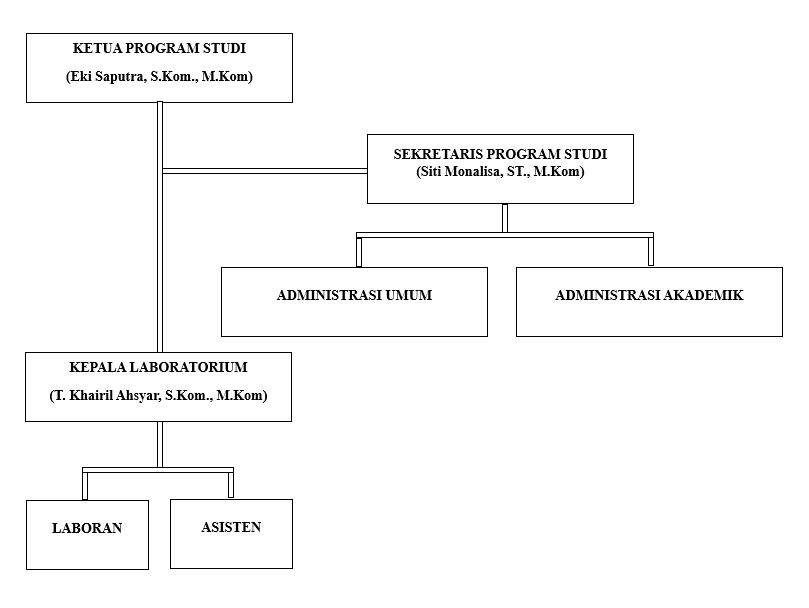
\includegraphics[width=0.82\linewidth]{konten//gambar/Struktur Organisasi.png}
	\caption{Struktur Organisasi Laboratorium}
	\label{fig:enter-label}
\end{figure}

%-----------------------------------------------------------------------------%
\section{Laboratorium}
Laboratorium merupakan sarana dalam melaksanakan sebuah riset dalam bidang ilmiah, eksperimen, pengukuran maupun pelatihan ilmiah. Meski laboratorium telah memiliki alat-alat yang lengkap, pengelolaan laboratorium juga harus diperhatikan. Adanya alat-alat yang sudah lengkap dan penggunaan yang sudah baik tentunya perlu untuk dilakukan manajemen yang baik pada laboratorium tersebut, karena terdapat beberapa hal yang harus diperhatikan kembali seperti pengelolaan masing-masing laboratorium dan pengolahan data \cite{sweden2022rancang}.

\subsection{Laboratorium Rekayasa Sistem Informasi (RSI)}
Laboratorium Rekayasa sistem Informasi atau yang disingkat dengan nama Laboratorium RSI merupakan laboratorium pertama yang dimiliki oleh Program Studi Sistem Informasi sejak pindahnya aktivitas perkuliahan kampus dari kampus Sukajadi ke kampus utama Panam Pekanbaru Riau pada tahun 2007. Fungsi utama dari laboratorium ini adalah sebagai fasilitas infrastruktur pendukung untuk pelaksanaan kegiatan perkuliahan praktikum bagi mahasiswa Program Studi Sistem Informasi terkait bidang Rekayasa Sistem Informasi. Bidang Rekayasa Sistem Informasi merupakan bidang yang paling dominan yang ada di Program Studi Sistem Informasi \cite{lab-si-website}.

\subsection{Laboratorium Internet (INT)}
Laboratorium Internet atau yang disingkat dengan nama Laboratorium INT merupakan laboratorium milik Program Studi Sistem Informasi di bawah Fakultas Sains dan Teknologi kedua yang aktivitas perkuliahannya berada di kampus utama Panam Pekanbaru Riau. Secara spesifik, laboratorium ini lebih dioperasikan untuk kebutuhan perkuliahan terkait matakuliah praktikum dasar, seperti matakuliah Jaringan Komputer dan Pemrograman Dasar \cite{lab-si-website}.

\subsection{Laboratorium \textit{Software Engineering} (SE)}
Laboratorium ke tiga yang dimiliki oleh Program Studi Sistem Informasi adalah Laboratorium \textit{Software Engineering} atau yang disingkat dengan nama Laboratorium SE. Laboratorium ini merupakan laboratorium terbaru milik yang dikelola oleh Program Studi dari usulan pengadaan barang tahun anggaran 2021 di bawah naungan Fakultas Sains dan Teknologi UIN Suska Riau. Adapun laboratorium SE sebagai pendukung dalam pelaksanaan kegiatan perkuliahan praktikum bagi mahasiswa Program Studi Sistem Informasi yang terkait dengan bidang keilmuan seperti Praktikum Basis Data, Pemrograman Beorientasi Objek (PBO), dan matakuliah wajib praktikum lainnya \cite{lab-si-website}.

\section{SITARIS SI}

Sistem Informasi Inventaris Laboratorium adalah sebuah platform yang dibuat dengan menggunakan Framework CodeIgniter4 dan bahasa pemrograman PHP yang dimaksudkan untuk membantu mengelola dan memantau inventaris barang dan peralatan laboratorium. Sistem ini memiliki potensi untuk meningkatkan efisiensi dan produktivitas dalam operasional laboratorium berkat berbagai fitur utama yang ditawarkannya.

Dengan adanya sistem ini, diharapkan pengelolaan inventaris laboratorium menjadi lebih mudah dan efisien, sehingga staf laboratorium dapat fokus pada tugas yang lebih penting. Selain itu, laporan yang dihasilkan oleh sistem dapat membantu dalam pengambilan keputusan yang lebih baik tentang persediaan barang dan peralatan laboratorium \cite{sitaris-lab-si-website}. SITARIS SI dapat diakses di alamat https://sitaris.lab-si.uin-suska.ac.id. Terdapat beberapa menu yang ada pada SITARIS SI, yaitu:

\begin{enumerate}
	\item Halaman \textit{login} \\ Halaman \textit{login} merupakan tampilan awal sistem ketika diakses. Terdapat formulir \textit{username} dan \textit{password} dan dilindungi oleh anti spam dari google reCAPTCHA yang digunakan untuk masuk ke dalam sistem informasi inventaris seperti pada Gambar 2.2.

	      \begin{figure}
		      \centering
		      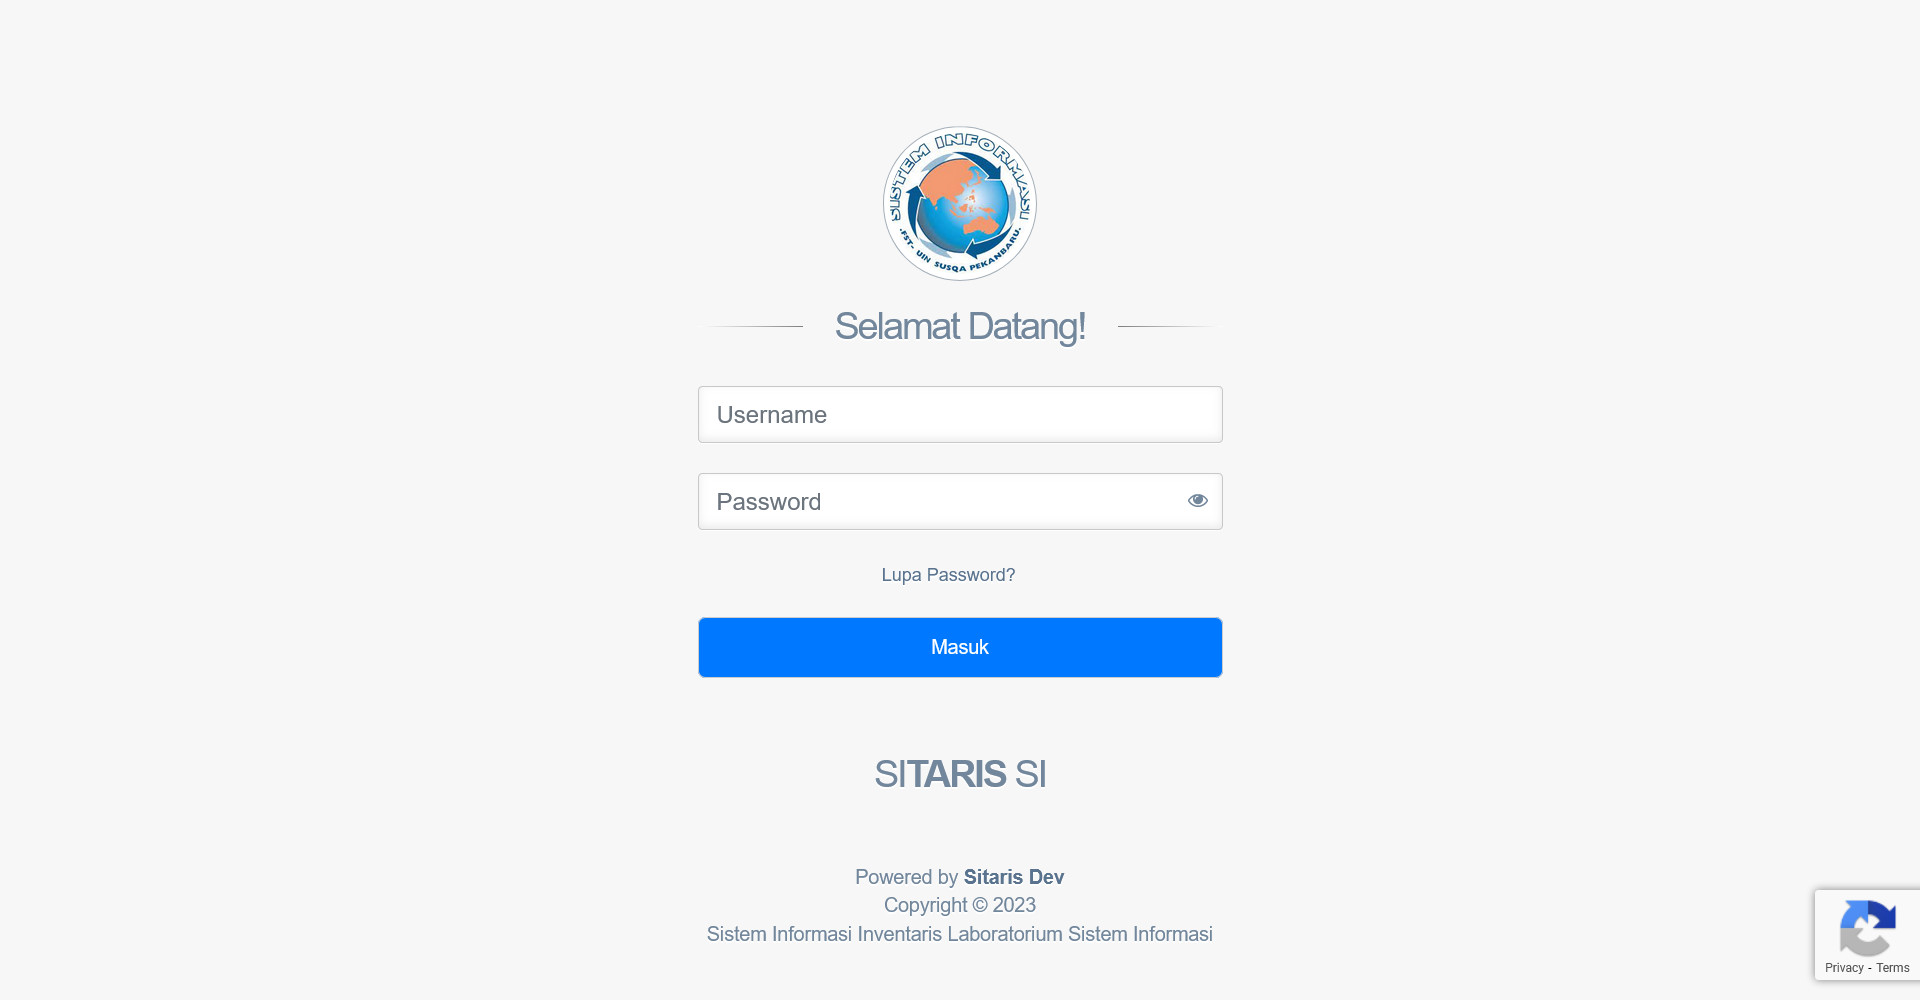
\includegraphics[width=0.82\linewidth]{konten//gambar/Login Page.png}
		      \caption{Halaman \textit{Login}}
		      \label{fig:enter-label}
	      \end{figure}

	\item Halaman Beranda \\ Halaman beranda merupakan tampilan awal yang ditampilkan kepada \textit{user} jika \textit{user} berhasil \textit{login} seperti pada Gambar 2.3.

	      \begin{figure}
		      \centering
		      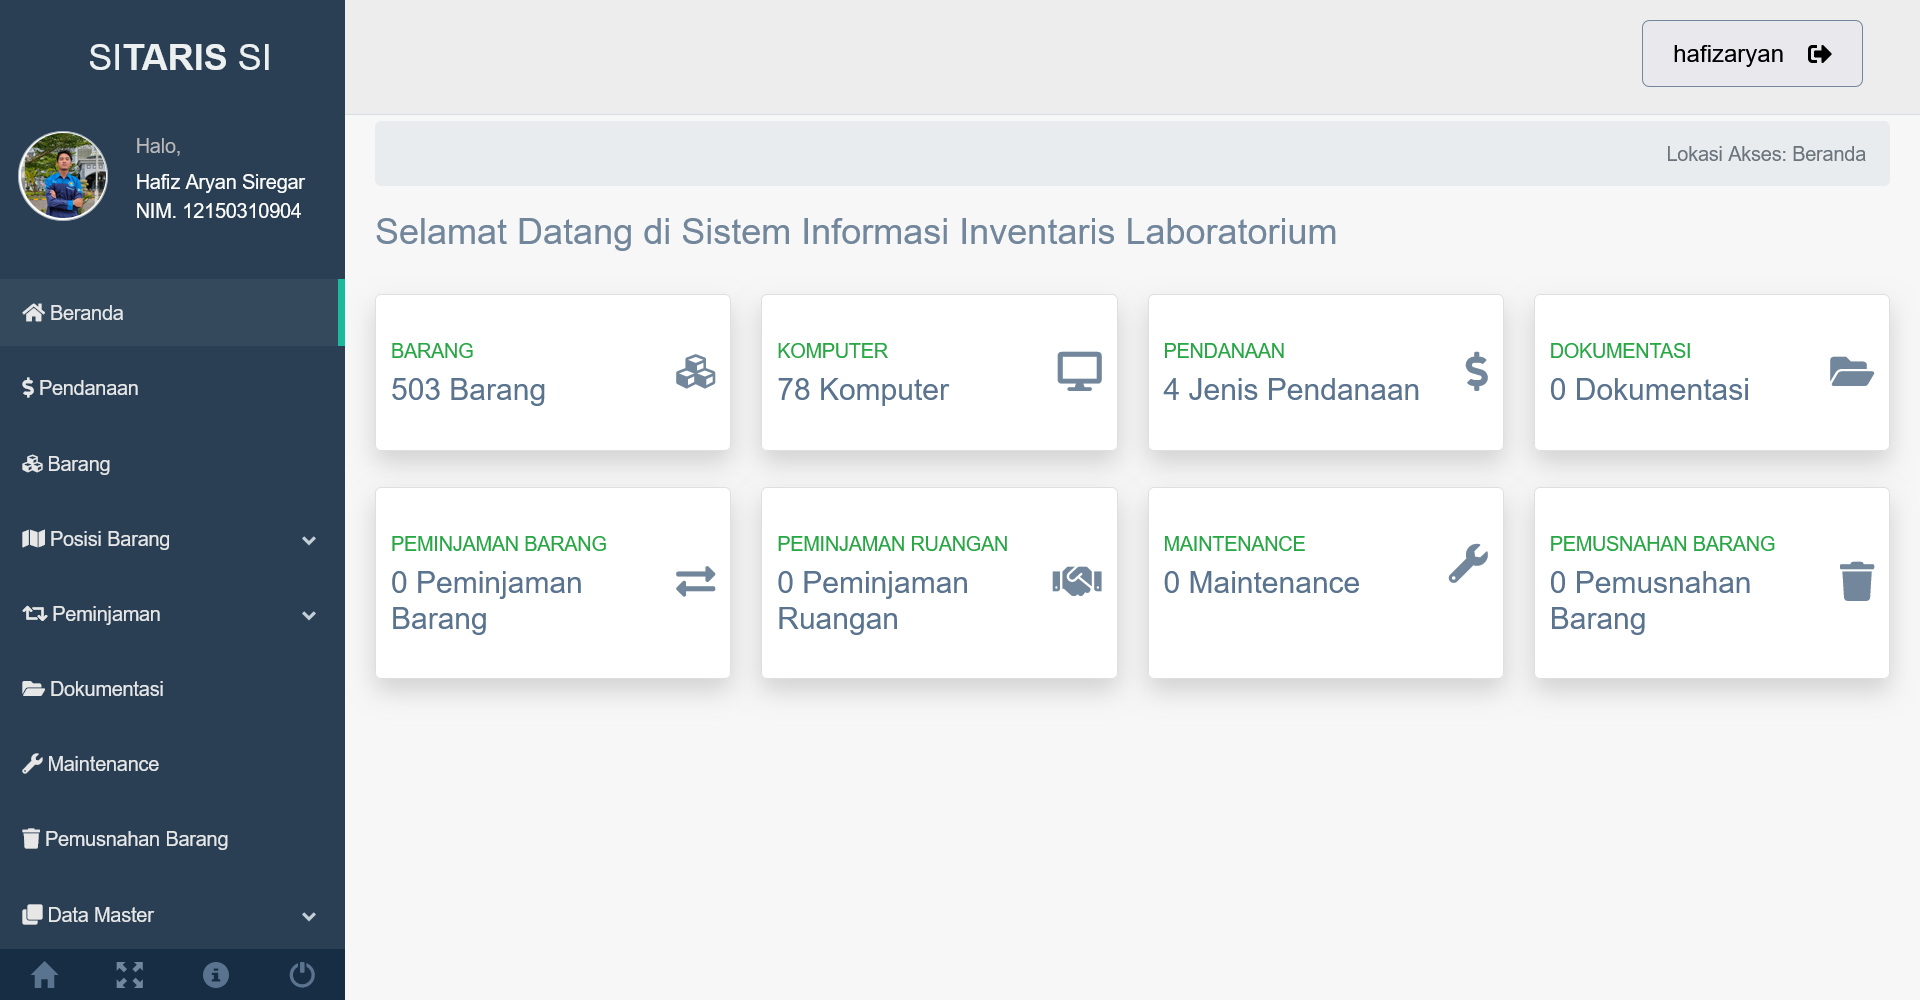
\includegraphics[width=0.82\linewidth]{konten//gambar/login berhasil.png}
		      \caption{Halaman Beranda}
		      \label{fig:enter-label}
	      \end{figure}

	\item Halaman Barang \\ Halaman barang merupakan tampilan untuk melihat dan mengelola data barang, tombol tambah data merupakan tombol yang dapat digunakan untuk beralih ke halaman tambah data barang, dan tombol pensil digunakan untuk mengedit data barang dan tombol \textit{trash} untuk menghapus data barang, lalu terdapat juga tombol berwarna biru toska yang dibedakan menjadi beberapa tombol yang bertujuan untuk mencetak dokumen laporan berdasarkan pendanaan, ruangan, kategori, tahun, dan QR seperti pada Gambar 2.7. sampai Gambar 2.19.

	      \begin{figure}
		      \centering
		      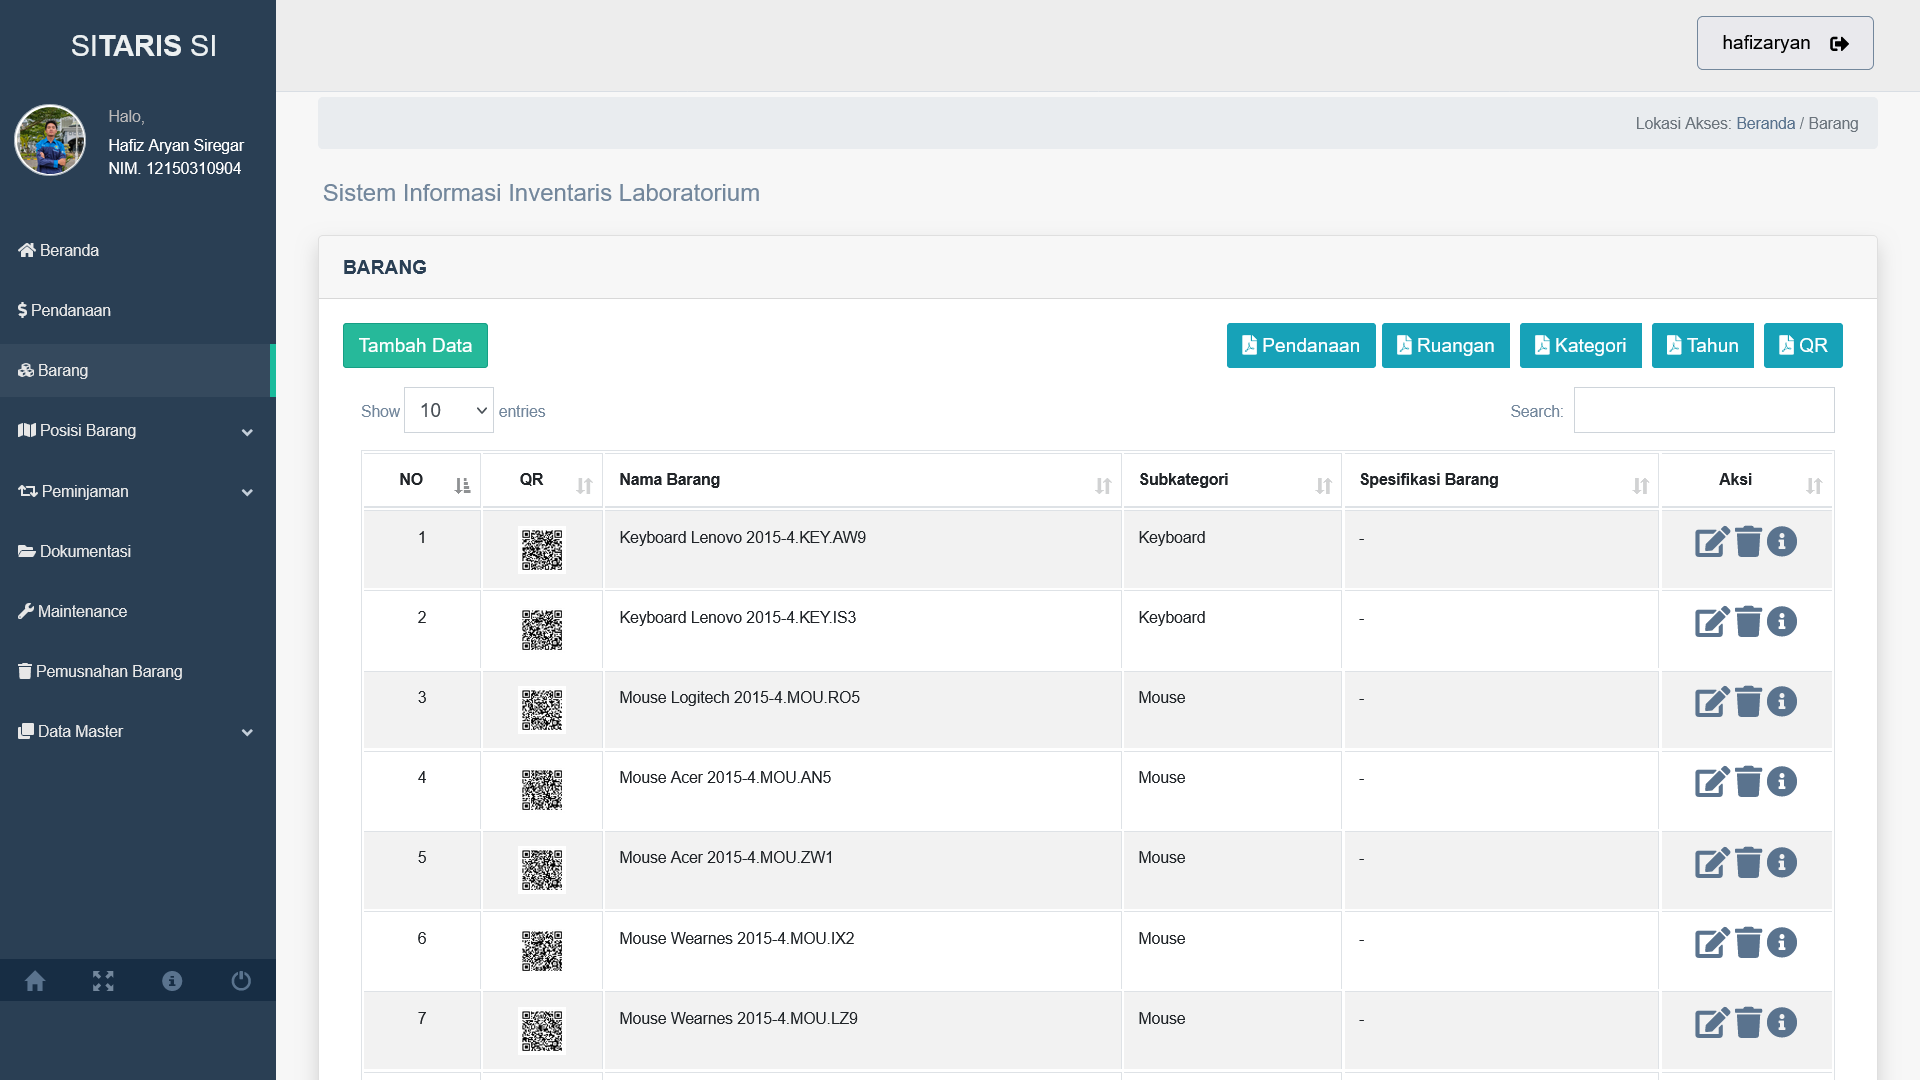
\includegraphics[width=0.82\linewidth]{konten//gambar/barang.png}
		      \caption{Halaman Barang \textit{Index}}
		      \label{fig:enter-label}
	      \end{figure}

\end{enumerate}

\section{Model Pengembangan Sistem}
Dalam penelitian ini, digunakan model pengembangan sistem Agile sebagai metodologi pengembangan perangkat lunak. Ada berbagai metode dan pendekatan pengembangan perangkat lunak tradisional seperti pendekatan waterfall, pendekatan iterative dan inkremental, pendekatan spiral, dan pendekatan evolutif. Pendekatan-pendekatan ini sering disebut sebagai pendekatan pengembangan perangkat lunak terencana atau pendekatan kelas berat. Pendekatan-pendekatan ini sangat berguna dalam mengembangkan perangkat lunak yang kompleks, membantu menghindari pengembangan perangkat lunak gaya lama yang informal dan memberikan perangkat lunak berkualitas tinggi secara sistematis, sehingga memenuhi persyaratan pengguna dalam batas waktu yang telah ditentukan \cite{al2020agile}.

\begin{figure}
	\centering
	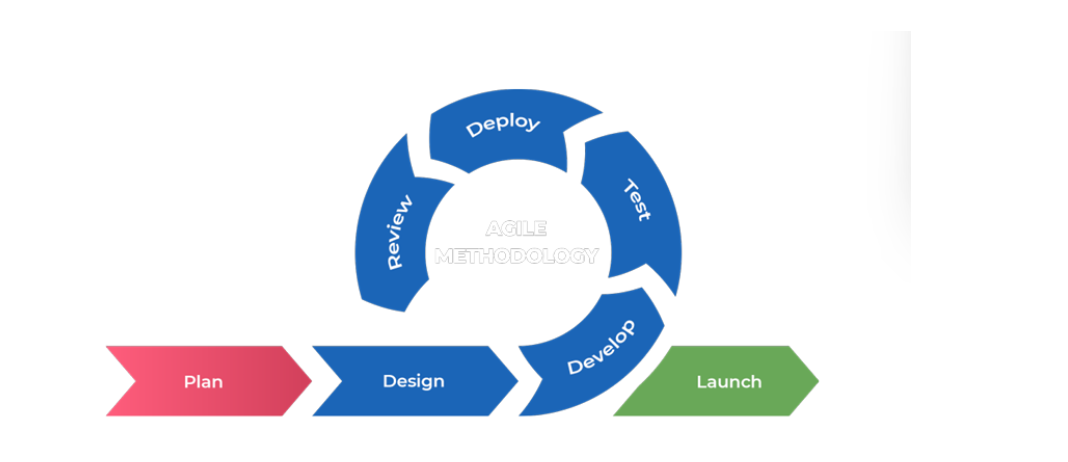
\includegraphics[width=0.82\linewidth]{konten//gambar/agile.png}
	\caption{\textit{Agile Development}}
	\label{fig:enter-label}
\end{figure}

% \section{Observasi}
% Observasi adalah tindakan mengamati secara langsung perilaku individu, objek, atau aktivitas dengan cara yang teratur tanpa melakukan interaksi lansung dengan subjek yang diamati. Observasi merupakan metode pengumpulan data di mana pengamat mengamati suatu sistem atau entitas saat sedang beroperasi untuk mendapatkan wawasan dan pemahaman yang lebih mendalam tentang bagaimana sistem tersebut bekerja \cite{tilley2017systems}.

\section{Web}
Rangkaian jaringan yang tersebar di seluruh dunia, yang di semua organisasi dihubungkan oleh jaringan terbesar sehingga dapat saling berkomunikasi,adalah istilah internet. Dengan Internet, pengguna dapat mengakses berbagai sistem dari mana saja, internet juga sebagai penghubung jaringan website. WorldWide Web (WWW) atau Website adalah laman-laman berisikan keterangan yang berada dalam taraf global berbasis hypertext yang memungkinkan pengguna mencari banyak sekali macam keterangan pada dunia selama terhubung menggunakan internet \cite{irawan2017implementasi}.

\section{PHP}
PHP (PHP: Hypertext Preprocessor) adalah bahasa pemrograman server-side yang digunakan untuk membuat situs web dinamis dan interaktif. PHP merupakan bahasa pemrograman yang populer dan mudah dipelajari, serta memiliki banyak fungsi yang dapat digunakan untuk membuat situs web yang interaktif dan dinamis. PHP dapat digunakan untuk membuat situs web yang interaktif, seperti form pendaftaran, login, dan lainnya. PHP juga dapat digunakan untuk membuat situs web yang dinamis, seperti situs web yang dapat menampilkan data dinamis dari database \cite{irawan2017implementasi}.

\section{Framework}
\textit{Framework} dalam pengembangan sistem adalah kerangka kerja atau struktur yang digunakan untuk memudahkan pengembangan aplikasi atau sistem \cite{sallaby2020perancangan}. \textit{Framework} menyediakan berbagai fitur dan fungsi yang dapat digunakan oleh pengembang untuk mempercepat proses pengembangan dan memastikan konsistensi dalam pengembangan aplikasi atau sistem \cite{simanullang2021sistem}. \textit{Framework} juga membantu pengembang dalam mengelola kode program dan memperbaiki \textit{bug}. Beberapa contoh \textit{framework} yang sering digunakan dalam pengembangan sistem adalah Laravel, CodeIgniter, dan beberapa \textit{framework} lainnya \cite{Fadllullah2022PengembanganSI}.

\section{CodeIgniter}
Codeigniter merupakan \textit{framework} untuk membangun aplikasi \textit{web} berbasis PHP. Codeigniter menyediakan banyak \textit{library} untuk fungsi-fungsi umum, antar muka yang sederhana, dan struktur yang logis. CodeIgniter menjadi sebuah \textit{framework} PHP dengan model MVC (Model, View, Controller) untuk membangun \textit{website} dinamis dengan menggunakan PHP yang dapat mempercepat pengembang untuk membuat sebuah aplikasi \textit{web}. Selain ringan dan cepat, CodeIgniter juga memiliki dokumentasi yang super lengkap disertai dengan contoh implementasi kode-nya. \textit{Programmer} dapat membuat aplikasi dengan lebih cepat karena tidak perlu menulis kode dari awal, selain itu Codeigniter juga menyediakan banyak fungsi yang siap digunakan. Seorang \textit{programmer} bisa lebih fokus dengan aplikasi yang sedang dibangun dan meminimalkan penulisan kode \cite{tyowati2017implementasi}.

\section{\textit{Database}}
\textit{Database} adalah suatu kumpulan data yang telah diatur secara terstruktur, memungkinkan akses dan pengelolaan melalui sistem komputer. Jenis data yang dapat disimpan di dalamnya mencakup teks, gambar, suara, dan video, dengan berbagai tujuan seperti penyimpanan informasi, analisis data, dan pengambilan keputusan. Untuk membuat dan mengelola \textit{database}, diperlukan perangkat lunak khusus seperti \textit{MariaDB}, \textit{Oracle}, atau \textit{Microsoft SQL Server} \cite{Cowls2021ADB}.

\section{MariaDB}
MariaDB adalah sistem manajemen basis data relasional (RDBMS) yang dapat dijalankan di server web. MariaDB adalah versi terbaru dari MySQL, yang merupakan sistem manajemen basis data relasional (RDBMS) yang populer untuk aplikasi web. MariaDB memiliki fitur yang mirip dengan MySQL, tetapi memiliki beberapa perbedaan dalam implementasi dan performa. MariaDB juga memiliki dokumentasi yang lengkap dan dukungan komunitas yang kuat, sehingga memudahkan pengembang untuk membuat dan mengembangkan aplikasi web yang berjalan di server MariaDB \cite{mariadb2024}.

\section{XAMPP}
XAMPP adalah sebuah paket lengkap untuk server web yang dapat dengan mudah diinstal di berbagai sistem operasi. Dalam paket ini sudah termasuk beberapa komponen penting seperti Apache (web server), MariaDB (database), PHP (server side scripting), dan berbagai pustaka pendukung lainnya. XAMPP dapat digunakan pada berbagai sistem operasi, termasuk Linux, Windows, MacOS, dan Solaris, sehingga memudahkan pembuatan server web multi-platform \cite{pakpahan2020sistem}.



%-----------------------------------------------------------------------------------------------%
%
% Maret 2019
% Template Latex untuk Tugas Akhir Program Studi Sistem informasi ini
% dikembangkan oleh Inggih Permana (inggihjava@gmail.com)
%
% Template ini dikembangkan dari template yang dibuat oleh Andreas Febrian (Fasilkom UI 2003).
%
% Orang yang cerdas adalah orang yang paling banyak mengingat kematian.
%
%-----------------------------------------------------------------------------------------------%


%-----------------------------------------------------------------------------%
\chapter{\babTiga}
%-----------------------------------------------------------------------------%
Kerangka penelitian ini adalah langkah demi langkah dalam penyusunan Tugas Akhir mulai dari Tahap Perencanaan penelitian hingga Tahap Hasil dan Dokumentasi. Berikut ini adalah gambar Metodologi Penelitian dapat dilihat pada Gambar 3.1.
\begin{figure}
	\centering
	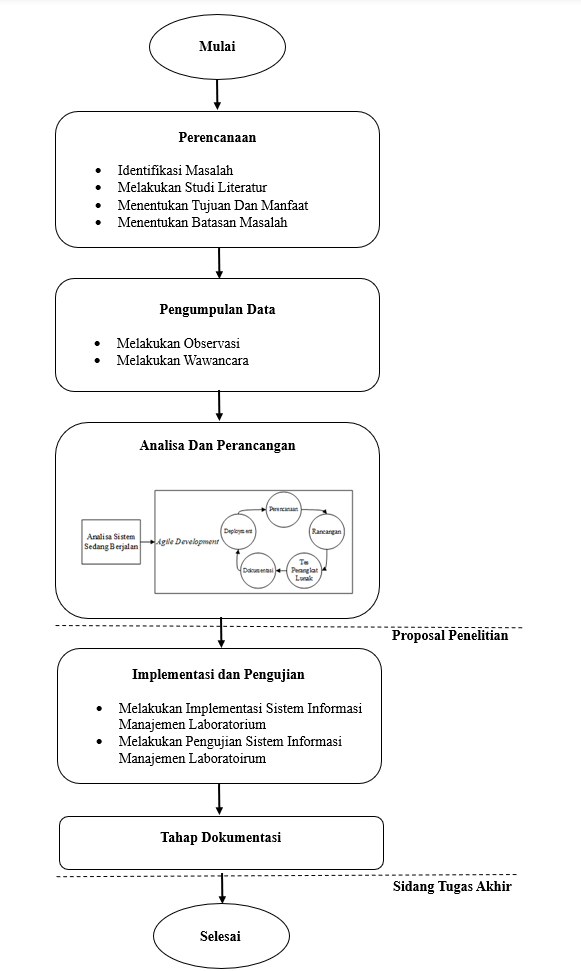
\includegraphics[width=0.82\linewidth]{konten//gambar/metodologi-penelitian.png}
	\caption{Metodologi Penelitian}
	\label{fig:enter-label}
\end{figure}
%-----------------------------------------------------------------------------%




\ifthenelse{\equal{\bidangta}{DUA}}{
	\renewcommand{\babEmpat}{ANALISIS DAN HASIL}
	\renewcommand{\babLima}{PENUTUP}
}{}

\ifthenelse{\equal{\tipeta}{PROPOSAL TUGAS AKHIR}}{
	\renewcommand{\babEmpat}{JANGKAAN HASIL}
}{}

%-----------------------------------------------------------------------------------------------%
%
% Maret 2019
% Template Latex untuk Tugas Akhir Program Studi Sistem informasi ini
% dikembangkan oleh Inggih Permana (inggihjava@gmail.com)
%
% Template ini dikembangkan dari template yang dibuat oleh Andreas Febrian (Fasilkom UI 2003).
%
% Orang yang cerdas adalah orang yang paling banyak mengingat kematian.
%
%-----------------------------------------------------------------------------------------------%


%-----------------------------------------------------------------------------%
\chapter{\babEmpat}
%-----------------------------------------------------------------------------%
\section{Analisis Sistem Berjalan}
Dalam proses tata kelola yang berlangsung di laboratorium Program Studi Sistem Informasi, hingga saat ini laboratorium telah menerapkan beberapa sistem informasi untuk mengelola berbagai aspek operasionalnya. Sistem-sistem tersebut meliputi:

\begin{enumerate}
	\item LAB SI \textit{Website} adalah sistem informasi yang berfungsi untuk mengelola informasi terkait laboratorium Program Studi Sistem Informasi, mencakup profil, informasi laboratorium, rilis media, pengumuman, dan galeri kegiatan.

	\item \textit{Laboratory Visitor Information System} yang disingkat LABVIS adalah sistem informasi yang digunakan untuk mengelola data kunjungan masuk dan keluar laboratorium, memungkinkan pemantauan dan pencatatan aktivitas pengunjung secara efisien.

	\item \textit{Laboratory Assistant Registration Information System} yang disingkat LARIS adalah sistem informasi yang digunakan untuk mengelola data pendaftar dan proses rekrutmen asisten laboratorium.

	\item Sistem Informasi Inventaris disingkat yang SITARIS adalah sistem informasi inventarisasi yang memfasilitasi pengelolaan dan pemantauan alat serta barang di laboratorium, meningkatkan efisiensi dalam manajemen inventaris.
\end{enumerate}

Implementasi sistem-sistem ini telah secara signifikan meningkatkan efektivitas dan efisiensi tata kelola laboratorium Program Studi Sistem Informasi, memungkinkan pengelolaan yang lebih terstruktur dan terintegrasi dalam berbagai aspek operasional laboratorium. Namun, beberapa sistem tersebut masih memiliki kekurangan dalam menunjang tata kelola laboratorium, terutama dalam hal penjadwalan. Saat ini, tidak ada sistem informasi yang secara khusus mengelola penjadwalan laboratorium Program Studi Sistem Informasi. Pengelolaan penjadwalan masih dilakukan secara manual dengan melakukan validasi dan pengecekan pada jadwal yang diperoleh dari Ketua Program Studi. Hal ini mengakibatkan ketidaksesuaian dan kurangnya informasi mengenai jadwal praktikum di laboratorium. Oleh karena itu, perlu dilakukan penyempurnaan pada sistem informasi yang ada, khususnya SITARIS, agar dapat memenuhi kebutuhan tata kelola laboratorium dalam hal penjadwalan ruangan. Penyempurnaan ini bertujuan untuk mencapai tujuan laboratorium dalam menerapkan \textit{Integrated Laboratory Management Information System} (ILMIS), yang akan mengintegrasikan seluruh aspek manajemen laboratorium, termasuk penjadwalan, ke dalam satu sistem yang efisien.

\section{Analisis Sistem Usulan}
Pengembangan sistem ini akan menyajikan fitur penjadwalan laboratorium yang dapat digunakan oleh Admin, Kaprodi, Sekprodi, dan Aslab. Fitur ini dirancang untuk mempermudah pengelolaan jadwal kegiatan di laboratorium, sehingga setiap pengguna dapat dengan mudah mengakses dan mengelola informasi terkait jadwal. Selain itu, sistem ini juga akan mengintegrasikan sistem informasi yang sudah ada seperti Website SI, LABVIS, dan LARIS. Dengan adanya sistem ini, diharapkan akan tercipta efisiensi dalam pengelolaan waktu dan sumber daya di laboratorium, serta mengurangi kemungkinan terjadinya bentrok jadwal antara berbagai kegiatan yang berlangsung dan juga mengintegrasikan sistem yang mulanya berdiri sendiri.

\section{Analisis Kebutuhan Sistem}
\subsection{Analisis Kebutuhan Fungsional Sistem}
Sistem ini dirancang untuk memenuhi berbagai kebutuhan fungsional yang esensial dalam pengelolaan penjadwalan laboratorium. Ini mencakup manajemen jadwal yang fleksibel dan mudah diakses, kemampuan pengelolaan jadwal yang intuitif dengan validasi yang ketat, serta sistem pengelolaan informasi yang memungkinkan pemantauan dan manajemen informasi terkait penggunaan laboratorium. Sistem ini juga mendukung proses validasi yang terstruktur  untuk memantau dan memberitahukan status penggunaan laboratorium kepada pengguna. Pengelolaan akses pengguna yang aman dan integrasi yang lancar dengan sistem internal laboratorium lainnya juga menjadi bagian integral dari fungsi sistem ini, memastikan efisiensi dan transparansi dalam seluruh proses penjadwalan laboratorium.

\subsection{Analisis Kebutuhan Non-Fungsional Sistem}
Kebutuhan non-fungsional sistem terbagi dalam dua kategori utama yaitu kebutuhan perangkat lunak dan kebutuhan perangkat keras. Analisis terhadap kebutuhan perangkat keras dilakukan untuk mengoptimalkan dan mempermudah proses perancangan serta implementasi sistem yang akan dibangun.
% -----------------------------------------------------------------------------%
\begin{enumerate}
	\item  Analisis Kebutuhan Perangkat Lunak \\
	      Pada tahap analisis ini, peneliti mengidentifikasi dan mendefinisikan segala kebutuhan yang harus dipenuhi oleh sistem yang akan dikembangkan. Fokus utama dari analisis ini adalah memahami secara mendalam tujuan dan kebutuhan pengguna akhir, baik itu admin, kalab, kaprodi, sekprodi dan aslab. Analisis kebutuhan perangkat lunak dapat dilihat pada Tabel \ref{tab:AnalisisKebutuhanPerangkatLunak}
	      \begin{longtable}{clcc}
		      \caption{Analisis Kebutuhan Perangkat Lunak}
		      \label{tab:AnalisisKebutuhanPerangkatLunak}                                                                                                               \\
		      \hline
		      \multicolumn{1}{l}{\textbf{No}} & \textbf{Perangkat Lunak}     & \multicolumn{1}{l}{\textbf{Versi Minimal}} & \multicolumn{1}{l}{\textbf{Versi Tersedia}} \\ \hline
		      \endfirsthead
		      %
		      \multicolumn{4}{c}%
		      {{\bfseries Table \thetable\ continued from previous page}}                                                                                               \\
		      \hline
		      \multicolumn{1}{l}{\textbf{No}} & \textbf{Perangkat Lunak}     & \multicolumn{1}{l}{\textbf{Versi Minimal}} & \multicolumn{1}{l}{\textbf{Versi Tersedia}} \\ \hline
		      \endhead
		      %
		      \hline
		      \endfoot
		      %
		      \endlastfoot
		      %
		      1                               & Windows                      & W8                                         & W11                                         \\
		      2                               & Balsamiq Mockup              & 4.0.0                                      & 4.7.5                                       \\
		      3                               & Google Chrome                & -                                          & 127.0.6533.100                              \\
		      4                               & MySQL                        & 8.0.0                                      & 8.0.30                                      \\
		      5                               & VS Code                      & 1.71.1                                     & 1.92.1                                      \\
		      6                               & Hypertext Preprocessor (PHP) & 8.0.0                                      & 8.2.16                                      \\
		      7                               & CodeIgniter                  & 4                                          & 4                                           \\ \hline
	      \end{longtable}

	\item Analisis Kebutuhan Perangkat Keras \\
	      Pada tahap analisis ini, peneliti melakukan identifikasi dan mendefinisikan segala kebutuhan yang harus dipenuhi oleh sistem yang dikembangkan. Fokus utama dari analisis ini adalah memahami secara mendalam tujuan dan kebutuhan pengguna akhir, baik admin, kalab, kaprodi, sekprodi, dan aslab. Analisis ini menjadi landasan kritis untuk merancang solusi yang tepat dan memastikan bahwa sistem dapat efektif memenuhi tujuan strategis laboratorium dalam mengelola manajemen tata kelola laboratorium. Analisis kebutuhan ini dapat dilihat pada Tabel \ref{tab:PerangkatKerasPengembang}.
	      \begin{longtable}{clll}
		      \caption{Analisis Kebutuhan Perangkat Keras Pengembang}
		      \label{tab:PerangkatKerasPengembang}                                                                                                                                                                                              \\
		      \hline
		      \textbf{No} & \multicolumn{1}{c}{\textbf{Perangkat Keras}} & \multicolumn{1}{c}{\textbf{Spesifikasi Minimal}}                          & \multicolumn{1}{c}{\textbf{Versi Tersedia}}                                              \\ \hline
		      \endfirsthead
		      %
		      \multicolumn{4}{c}%
		      {{\bfseries Table \thetable\ continued from previous page}}                                                                                                                                                                       \\
		      \hline
		      \textbf{No} & \multicolumn{1}{c}{\textbf{Perangkat Keras}} & \multicolumn{1}{c}{\textbf{Spesifikasi Minimal}}                          & \multicolumn{1}{c}{\textbf{Versi Tersedia}}                                              \\ \hline
		      \endhead
		      %
		      \hline
		      \endfoot
		      %
		      \endlastfoot
		      %
		      1           & Processor                                    & \begin{tabular}[c]{@{}l@{}}Intel Core i3 atau AMD \\ Ryzen 3\end{tabular} & \begin{tabular}[c]{@{}l@{}}AMD Ryzen 5 5600U, 6Cores, \\ 12Threads, 2.3GHz.\end{tabular} \\
		      2           & Memory                                       & 4 GB DDR4                                                                 & 16 GB DDR4-3200 MHz                                                                      \\
		      3           & Storage                                      & \begin{tabular}[c]{@{}l@{}}256 GB SSD atau \\ 500 GB HDD\end{tabular}     & 512 GB M.2 NVMe                                                                          \\
		      4           & Keyboard                                     & \begin{tabular}[c]{@{}l@{}}Standard QWERTY \\ keyboard\end{tabular}       & 6-row, multimedia Fn keys                                                                \\
		      5           & Connection                                   & \begin{tabular}[c]{@{}l@{}}Wi-Fi 802.11n atau \\ Ethernet\end{tabular}    & Wi-Fi® 6                                                                                 \\
		      6           & Monitor                                      & \begin{tabular}[c]{@{}l@{}}14 inch, resolusi \\ 1366x768\end{tabular}     & 13 inc                                                                                   \\ \hline
	      \end{longtable}

	      Dalam spesifikasi perangkat keras yang disarankan pada Sistem \textit{Integrated Laboratory Management Information System} sesuai yang tertera pada Tabel \ref{tab:PerangkatKerasPengembang} sebaiknya memenuhi syarat spesifikasi minimum agar sistem dapat berjalan dengan sempurna.

\end{enumerate}

% =======================================================================================================================
\section{Perancangan}
Perancangan sistem perlu dilakukan sebelum dilakukan pembuatan sistem. tujuan dari perancangan sistem adalah untuk menentukan, mengorganisir, dan membentuk komponen dari solusi sistem akhir sehingga memiliki \textit{blueprint} untuk membangun sistem.

% =======================================================================================================================
\subsection{Use Case Diagram}
\textit{\textit{Use case} diagram} terdiri dari \textit{actor}, \textit{use case} dan serta hubungannya. \textit{\textit{Use case} diagram} adalah sesuatu yang penting untuk memvisualisasiakan, menspesifikasikan dan mendokumentasikan kebutuhan perilaku sistem. \textit{\textit{Use case} diagram} digunakan untuk menjelaskan kegiatan apa saja yang dapat dilakukan oleh \textit{user} pengguna sistem yang sedang berjalan \cite{Carstoiu1995}.
\begin{longtable}{clp{8cm}}
	\caption{Deskripsi Aktor}
	\label{tab:DeskripsiAktor}                                                                                                    \\
	\hline
	\textbf{No} & \multicolumn{1}{c}{\textbf{Aktor}} & \multicolumn{1}{c}{\textbf{Deskripsi}}                                     \\ \hline
	\endfirsthead
	%
	\multicolumn{3}{c}%
	{{\bfseries Tabel \thetable\ lanjutan dari halaman sebelumnya}}                                                               \\
	\hline
	\textbf{No} & \multicolumn{1}{c}{\textbf{Aktor}} & \multicolumn{1}{c}{\textbf{Deskripsi}}                                     \\ \hline
	\endhead
	%
	\hline
	\endfoot
	%
	\endlastfoot
	%
	1           & Admin                              & Mengelola penjadwalan laboratorium termasuk lihat, tambah, edit, dan hapus \\
	2           & Kalab                              & Mengelola penjadwalan laboratorium termasuk lihat, tambah, edit, dan hapus \\
	3           & Kaprodi                            & Melihat penjadwalan laboratorium                                           \\
	4           & Sekprodi                           & Melihat penjadwalan laboratorium                                           \\
	5           & Aslab                              & Mengelola penjadwalan laboratorium termasuk lihat, tambah, edit, dan hapus \\ \hline
\end{longtable}

Sistem manajemen laboratorium adalah sistem yang terkonsentrasi diurus oleh seseorang dengan peran Admin. Jenis ini digambarkan menggunakan diagram use case yang terlihat pada aktivitas interternal admin sistem dengan komponen yang ada.

Dengan sistem ini terdapat 4 fungsi substansial yang dapat dipergunakan oleh adm selama mengoperasikan peralatan sistem. Fungsi - fungsi tersebut yaitu kompetensi Admin untuk menambah jadwal baru melalui menu "Tambah Jadwal Laboratorium", Edit jadwal yang bersistem dengan "Edit Jadwal Laboratorium", Menghapus schedule yang tidak diinginkan dengan "Hapus Jadwal Laboratorium", dan menampilkan history schedule dengan menjual "Lihat Jadwal Laboratorium"

Keamanan sistem dijamin melalui mekanisme login yang ditunjukkan dengan relasi “include” pada diagram. Tiga fungsi utama yaitu penambahan, pengeditan, dan penghapusan jadwal termasuk kedalam scope otoritas Adm, oleh sebab itu fungsi ini harus log in terlebih dahulu saat meta ternotfied. Sementara itu fungsi melihat jadual bagi pelaksana lab tidak mensyaratkan kuliah dahulu seperti yang ternyata dalam Gambar

\ref{usecase-diagram-admin}.
\begin{figure}
	\centering
	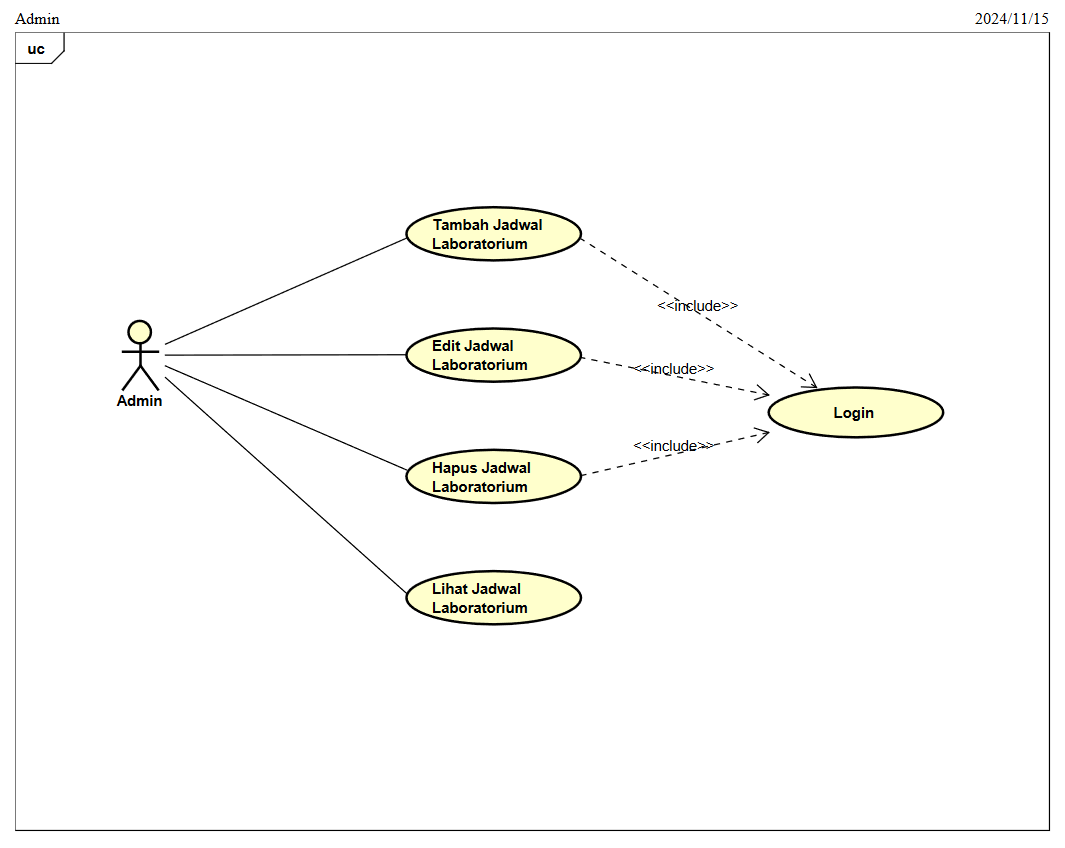
\includegraphics[width=0.82\textwidth]{konten/gambar/usecase-diagram/admin.png}
	\caption{\textit{Usecase Diagram} Admin}
	\label{usecase-diagram-admin}
\end{figure}

Dalam sistem ini, Kalab memiliki empat fungsi utama yang dapat diakses. Fungsi-fungsi tersebut meliputi kemampuan untuk menambahkan jadwal baru melalui fitur "Tambah Jadwal Laboratorium", melakukan perubahan pada jadwal yang sudah ada menggunakan fitur "Edit Jadwal Laboratorium", menghapus jadwal yang tidak diperlukan dengan fitur "Hapus Jadwal Laboratorium", dan melihat seluruh daftar jadwal yang tersedia melalui fitur "Lihat Jadwal Laboratorium".

Keamanan sistem dijamin melalui mekanisme login yang ditunjukkan dengan relasi "include" pada diagram. Tiga fungsi utama, yaitu menambah, mengedit, dan menghapus jadwal, mengharuskan Kalab untuk melakukan login terlebih dahulu sebelum dapat mengakses fungsi-fungsi tersebut. Sementara itu, fungsi untuk melihat jadwal laboratorium dapat diakses secara langsung tanpa perlu melalui proses login terlebih dahulu, seperti yang ditunjukkan pada Gambar \ref{usecase-diagram-kalab}.
\begin{figure}
	\centering
	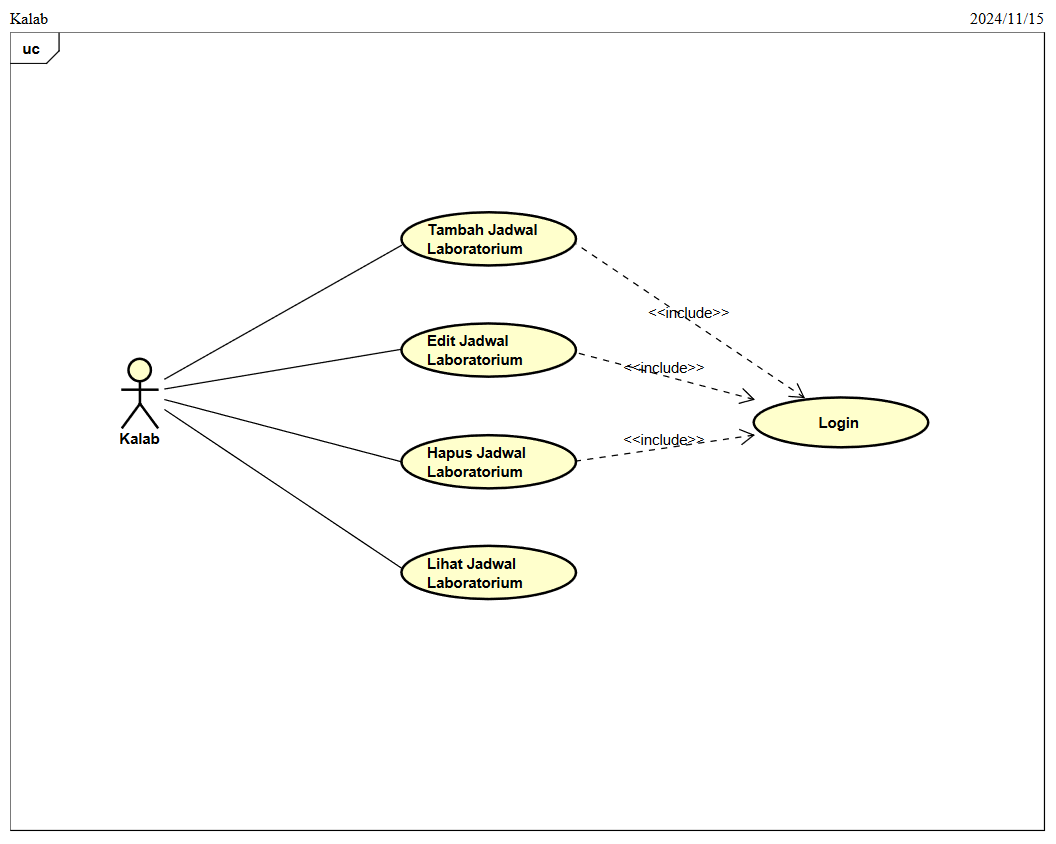
\includegraphics[width=0.82\textwidth]{konten/gambar/usecase-diagram/kalab.png}
	\caption{\textit{Usecase Diagram} Kalab}
	\label{usecase-diagram-kalab}
\end{figure}

Dalam sistem ini, Kaprodi memiliki satu fungsi utama yang dapat diakses, yaitu melihat seluruh daftar jadwal yang tersedia melalui fitur "Lihat Jadwal Laboratorium".

Fungsi ini dapat diakses secara langsung tanpa perlu melalui proses login terlebih dahulu, sehingga Kaprodi dapat dengan mudah memantau jadwal laboratorium yang ada. Hal ini ditunjukkan pada Gambar \ref{usecase-diagram-kaprodi}.
\begin{figure}
	\centering
	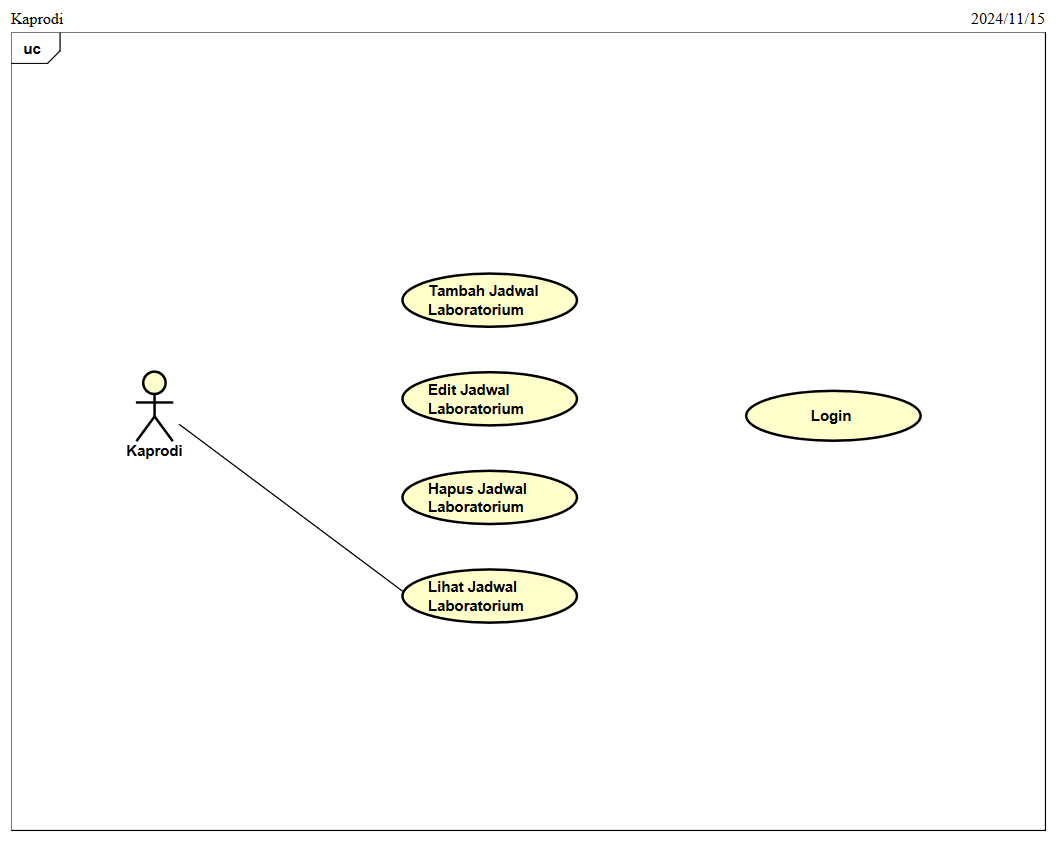
\includegraphics[width=0.82\textwidth]{konten/gambar/usecase-diagram/kaprodi.png}
	\caption{\textit{Usecase Diagram} Kaprodi}
	\label{usecase-diagram-kaprodi}
\end{figure}

Dalam sistem ini, Sekprodi memiliki satu fungsi utama yang dapat diakses, yaitu melihat seluruh daftar jadwal yang tersedia melalui fitur "Lihat Jadwal Laboratorium".

Fungsi ini dapat diakses secara langsung tanpa perlu melalui proses login terlebih dahulu, sehingga Sekprodi dapat dengan mudah memantau jadwal laboratorium yang ada. Hal ini ditunjukkan pada Gambar \ref{usecase-diagram-sekprodi}.
\begin{figure}
	\centering
	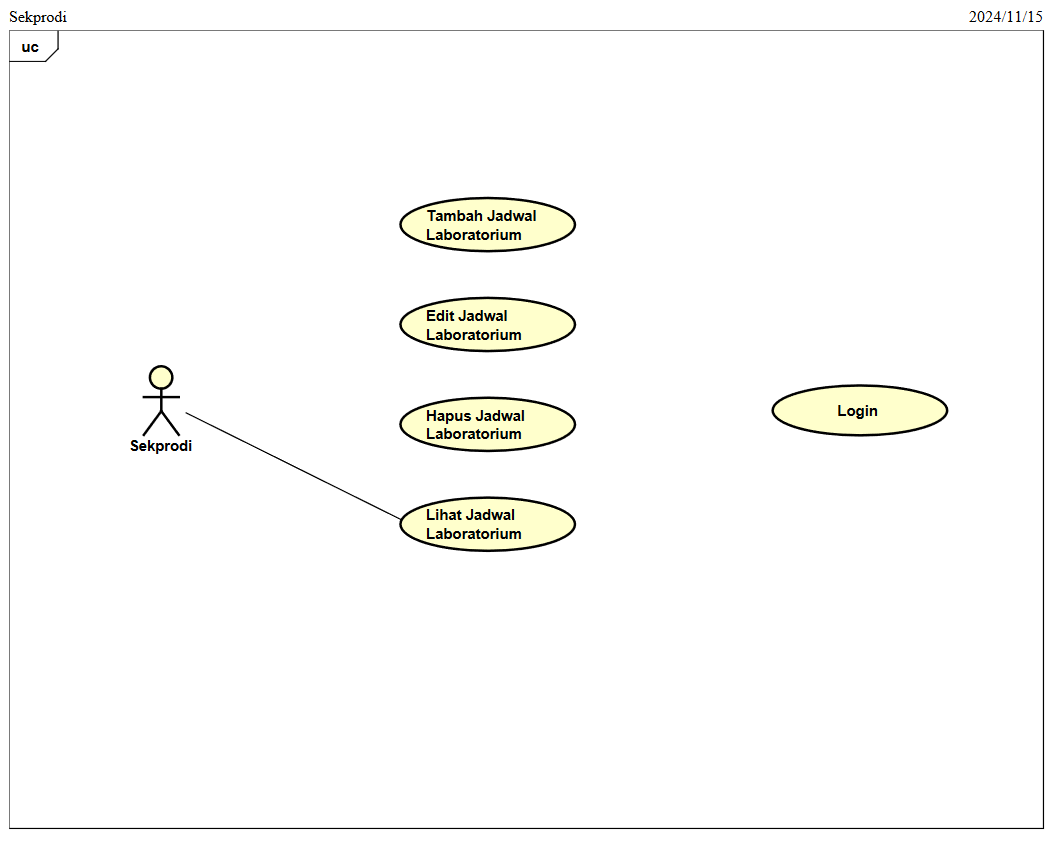
\includegraphics[width=0.82\textwidth]{konten/gambar/usecase-diagram/sekprodi.png}
	\caption{\textit{Usecase Diagram} Sekprodi}
	\label{usecase-diagram-sekprodi}
\end{figure}

Dalam sistem ini, Kalab memiliki empat fungsi utama yang dapat diakses. Fungsi-fungsi tersebut meliputi kemampuan untuk menambahkan jadwal baru melalui fitur "Tambah Jadwal Laboratorium", melakukan perubahan pada jadwal yang sudah ada menggunakan fitur "Edit Jadwal Laboratorium", menghapus jadwal yang tidak diperlukan dengan fitur "Hapus Jadwal Laboratorium", dan melihat seluruh daftar jadwal yang tersedia melalui fitur "Lihat Jadwal Laboratorium".

Keamanan sistem dijamin melalui mekanisme login yang ditunjukkan dengan relasi "include" pada diagram. Tiga fungsi utama, yaitu menambah, mengedit, dan menghapus jadwal, mengharuskan Kalab untuk melakukan login terlebih dahulu sebelum dapat mengakses fungsi-fungsi tersebut. Sementara itu, fungsi untuk melihat jadwal laboratorium dapat diakses secara langsung tanpa perlu melalui proses login terlebih dahulu, seperti yang ditunjukkan pada Gambar \ref{usecase-diagram-kalab}.
\begin{figure}
	\centering
	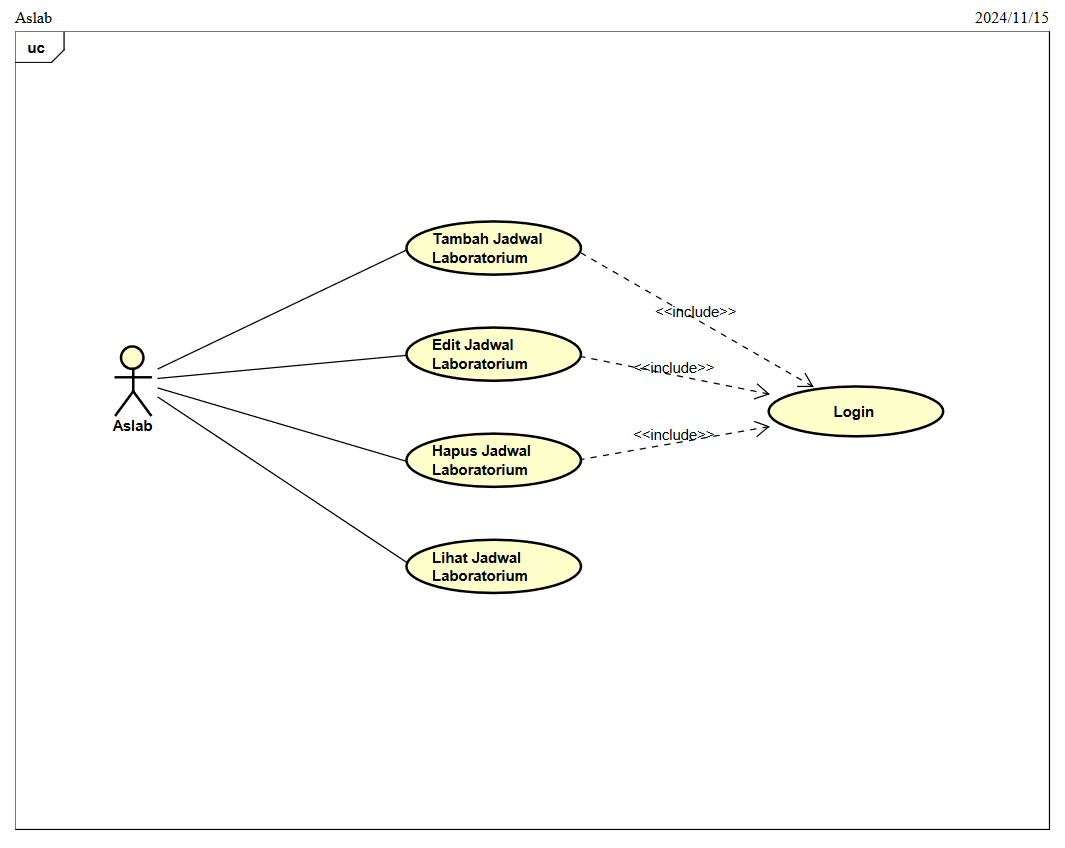
\includegraphics[width=0.82\textwidth]{konten/gambar/usecase-diagram/aslab.png}
	\caption{\textit{Usecase Diagram} Aslab}
	\label{usecase-diagram-aslab}
\end{figure}

% Skenario \textit{use case Login} merujuk pada rangkaian langkah-langkah terstruktur yang harus dilakukan oleh pengguna untuk melakukan proses kegiatan dalam suatu sistem. Proses ini dimulai dengan pengguna yang ingin mengakses sistem harus memasukkan informasi identifikasi pribadi, seperti nim, dan kata sandi, guna memverifikasi identitas mereka. Setelah pengisian data, sistem akan melakukan verifikasi dengan data yang tercatat dalam basis data, dan jika sesuai, pengguna akan diberikan izin akses ke fitur atau informasi yang relevan. Skenario \textit{Use Case Login} memegang peran krusial dalam menjaga tingkat keamanan serta privasi sistem, menjamin bahwa hanya pengguna yang diberi akses yang dapat masuk kedalam sistem.

% Pentingnya tahap ini dalam keamanan sistem ditunjukkan dalam Tabel \ref{tab:SkenarioLogin} yang secara rinci menggambarkan langkah-langkah dalam proses otentikasi. Dengan menjamin kelancaran proses ini, sistem dapat melindungi data sensitif dan memastikan bahwa hanya pengguna yang berwenang yang memiliki akses ke informasi yang terdapat dalam sistem.

% 	{
% 		\fontsize{10}{12}
% 		\begin{longtable}{@{} p{6cm} p{6cm} @{}}
% 			\caption{Skenario \textit{Use Case Login}} \label{tab:SkenarioLogin}                                                                                                                                                                                                           \\ \hline
% 			\textbf{Nama use case}                                                                         & \textit{Login}                                                                                                                                                                \\
% 			\textbf{Aktor}                                                                                 & Admin, Kalab, Aslab, Pendaftar.                                                                                                                                               \\
% 			\textbf{Deskripsi}                                                                             & \textit{Use case} ini menggambarkan untuk dapat mengelola sistem, Admin, Kepala Laboratorium, Pendaftar, Asisten Laboratorium harus melakukan \textit{login} terlebih dahulu. \\
% 			\textbf{Kondisi Awal}                                                                          & Sistem menampilkan form \textit{login}.                                                                                                                                       \\
% 			\textbf{Kondisi Akhir}                                                                         & Sistem menampilkan menu utama.                                                                                                                                                \\ \hline
% 			\multicolumn{1}{c}{\textbf{Aktor}}                                                             & \multicolumn{1}{c}{\textbf{Sistem}}                                                                                                                                           \\ \hline
% 			\multicolumn{2}{c}{\textbf{Skenario normal}}                                                                                                                                                                                                                                   \\ \hline
% 			1. \textit{Use case} ini dimulai ketika Admin, Kalab, Kaprodi, Sekprodi, Aslab \textit{login}. &                                                                                                                                                                               \\
% 			                                                                                               & 2. Sistem melakukan verifikasi \textit{login}.                                                                                                                                \\
% 			                                                                                               & 3. Sistem menampilkan menu utama.                                                                                                                                             \\ \hline
% 			\multicolumn{2}{c}{\textbf{Skenario gagal}}                                                                                                                                                                                                                                    \\ \hline
% 			1. \textit{Use case} ini dimulai ketika Admin, Kalab, Kaprodi, Sekprodi, Aslab \textit{login}. &                                                                                                                                                                               \\
% 			                                                                                               & 2. Sistem melakukan verifikasi \textit{login}.                                                                                                                                \\
% 			                                                                                               & 3. Sistem menampilkan pesan \textit{login} tidak valid.                                                                                                                       \\ \hline
% 		\end{longtable}}

% 	{
% 		\fontsize{10}{12}
% 		\begin{longtable}{@{} p{6cm} p{6cm} @{}}
% 			\caption{Skenario \textit{Use Case Kalab}} \label{tab:SkenarioKalab}                                                                                                                                             \\ \hline
% 			\textbf{Nama use case}                            & \textit{Manajemen Jadwal Laboratorium}                                                                                                                       \\
% 			\textbf{Aktor}                                    & Kalab, Aslab.                                                                                                                                                \\
% 			\textbf{Deskripsi}                                & \textit{Use case} ini menggambarkan proses yang dilakukan oleh Kalab untuk mengelola jadwal laboratorium, termasuk menambah, mengedit, dan menghapus jadwal. \\
% 			\textbf{Kondisi Awal}                             & Sistem menampilkan menu manajemen jadwal.                                                                                                                    \\
% 			\textbf{Kondisi Akhir}                            & Sistem menampilkan daftar jadwal laboratorium yang telah diperbarui.                                                                                         \\ \hline
% 			\multicolumn{1}{c}{\textbf{Aktor}}                & \multicolumn{1}{c}{\textbf{Sistem}}                                                                                                                          \\ \hline
% 			\multicolumn{2}{c}{\textbf{Skenario normal}}                                                                                                                                                                     \\ \hline
% 			1. Kalab memilih opsi untuk menambah jadwal baru. &                                                                                                                                                              \\
% 			                                                  & 2. Sistem menampilkan form untuk input jadwal baru.                                                                                                          \\
% 			                                                  & 3. Kalab mengisi form dan mengirimkan data.                                                                                                                  \\
% 			                                                  & 4. Sistem menyimpan jadwal baru dan menampilkan konfirmasi.                                                                                                  \\ \hline
% 			\multicolumn{2}{c}{\textbf{Skenario gagal}}                                                                                                                                                                      \\ \hline
% 			1. Kalab memilih opsi untuk menambah jadwal baru. &                                                                                                                                                              \\
% 			                                                  & 2. Sistem menampilkan form untuk input jadwal baru.                                                                                                          \\
% 			                                                  & 3. Kalab mengisi form dengan data yang tidak valid.                                                                                                          \\
% 			                                                  & 4. Sistem menampilkan pesan kesalahan dan meminta Kalab untuk memperbaiki data.                                                                              \\ \hline
% 		\end{longtable}}
% 	{

% 		\fontsize{10}{12}
% 		\begin{longtable}{@{} p{6cm} p{6cm} @{}}
% 			\caption{Skenario \textit{Use Case Kalab}} \label{tab:SkenarioKalab}                                                                                                                                             \\ \hline
% 			\textbf{Nama use case}                            & \textit{Manajemen Jadwal Laboratorium}                                                                                                                       \\
% 			\textbf{Aktor}                                    & Kalab, Aslab.                                                                                                                                                \\
% 			\textbf{Deskripsi}                                & \textit{Use case} ini menggambarkan proses yang dilakukan oleh Kalab untuk mengelola jadwal laboratorium, termasuk menambah, mengedit, dan menghapus jadwal. \\
% 			\textbf{Kondisi Awal}                             & Sistem menampilkan menu manajemen jadwal.                                                                                                                    \\
% 			\textbf{Kondisi Akhir}                            & Sistem menampilkan daftar jadwal laboratorium yang telah diperbarui.                                                                                         \\ \hline
% 			\multicolumn{1}{c}{\textbf{Aktor}}                & \multicolumn{1}{c}{\textbf{Sistem}}                                                                                                                          \\ \hline
% 			\multicolumn{2}{c}{\textbf{Skenario normal}}                                                                                                                                                                     \\ \hline
% 			1. Kalab memilih opsi untuk menambah jadwal baru. &                                                                                                                                                              \\
% 			                                                  & 2. Sistem menampilkan form untuk input jadwal baru.                                                                                                          \\
% 			                                                  & 3. Kalab mengisi form dan mengirimkan data.                                                                                                                  \\
% 			                                                  & 4. Sistem menyimpan jadwal baru dan menampilkan konfirmasi.                                                                                                  \\ \hline
% 			\multicolumn{2}{c}{\textbf{Skenario gagal}}                                                                                                                                                                      \\ \hline
% 			1. Kalab memilih opsi untuk menambah jadwal baru. &                                                                                                                                                              \\
% 			                                                  & 2. Sistem menampilkan form untuk input jadwal baru.                                                                                                          \\
% 			                                                  & 3. Kalab mengisi form dengan data yang tidak valid.                                                                                                          \\
% 			                                                  & 4. Sistem menampilkan pesan kesalahan dan meminta Kalab untuk memperbaiki data.                                                                              \\ \hline
% 		\end{longtable}}

% =======================================================================================================================
\subsection{\textit{Activity Diagram}}
\textit{Activity diagram} adalah salah satu alat dalam \textit{Unified Modeling Language} (UML) yang digunakan untuk memvisualisasikan alur kerja atau aktivitas dalam suatu sistem \cite{linzhang2004generating}. Pada sistem ini, \textit{activity diagram} memberikan gambaran rinci tentang proses yang dilalui oleh berbagai aktor seperti Admin, Kalab, Kaprodi, Sekprodi, Aslab.

\textit{Activity diagram} login memberikan gambaran rinci tentang proses login yang dilalui oleh pengguna. Diagram ini memandu langkah-langkah yang terlibat dalam proses login, mulai dari input data oleh pengguna, validasi oleh sistem hingga dapat masuk ke dalam sistem menggunakan akun yang sudah ada. \textit{Activity diagram} ini dapat dilihat pada Gambar \ref{activity-diagram-login}.
\begin{figure}
	\centering
	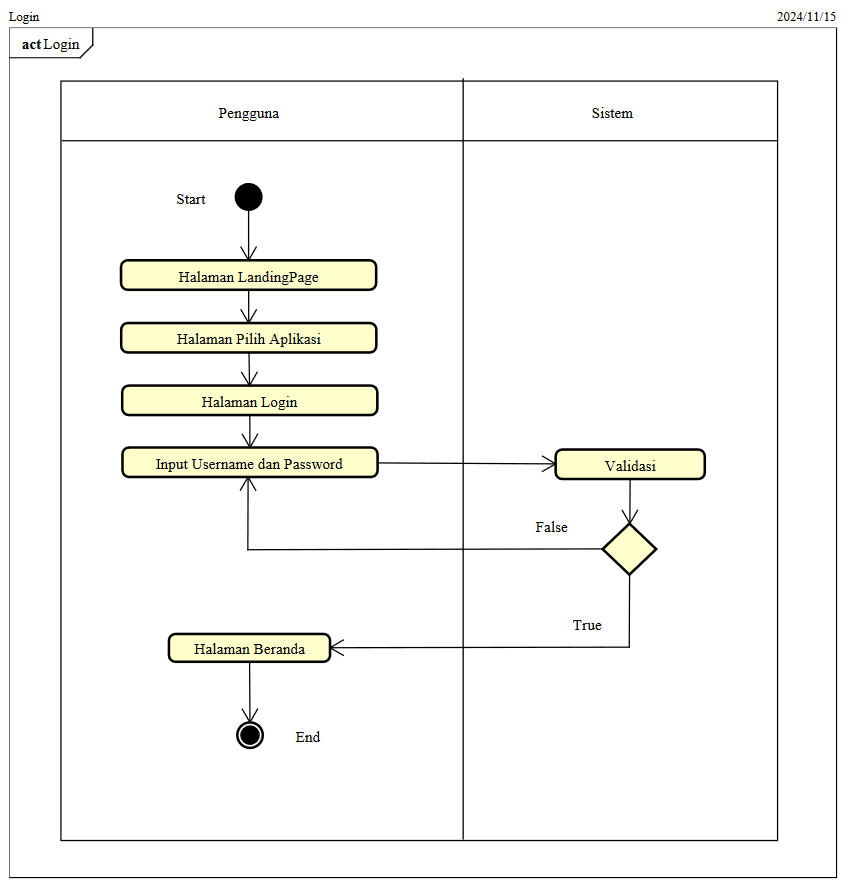
\includegraphics[width=0.82\textwidth]{konten/gambar/activity-diagram/login.png}
	\caption{\textit{Activity Diagram} Login}
	\label{activity-diagram-login}
\end{figure}

\textit{Activity diagram} tambah dosen memberikan gambaran rinci tentang proses penambahan dosen yang dilalui oleh pengguna. Diagram ini memandu langkah-langkah yang terlibat dalam proses penambahan dosen, mulai dari input data oleh pengguna, validasi oleh sistem hingga penyimpanan data dosen baru ke dalam sistem. \textit{Activity diagram} ini dapat dilihat pada Gambar \ref{activity-diagram-tambah-dosen}.
\begin{figure}
	\centering
	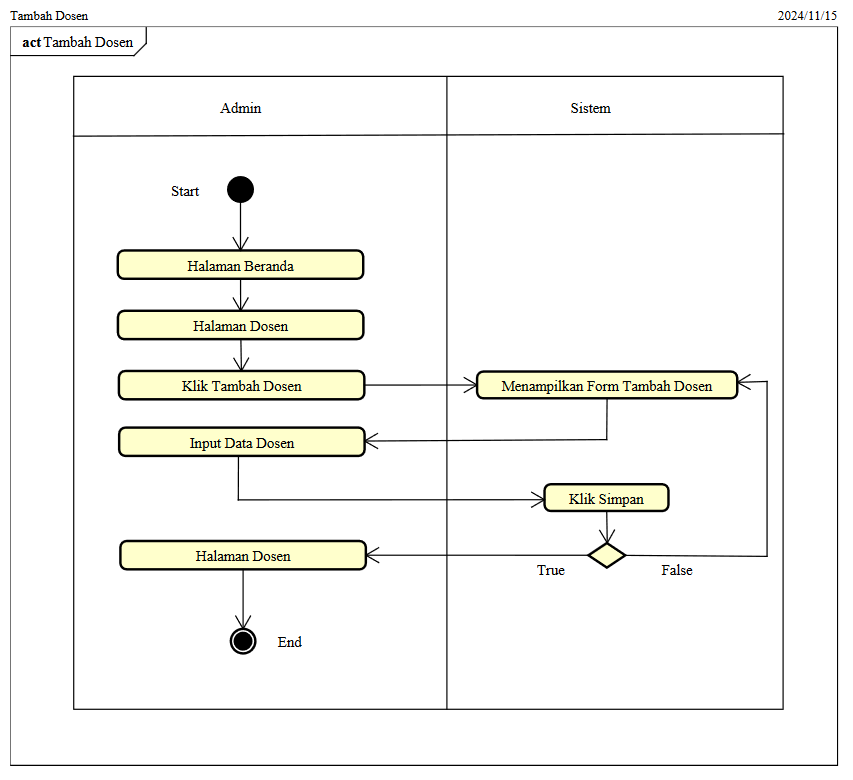
\includegraphics[width=0.82\textwidth]{konten/gambar/activity-diagram/tambah-dosen.png}
	\caption{\textit{Activity Diagram} Tambah Dosen}
	\label{activity-diagram-tambah-dosen}
\end{figure}

\textit{Activity diagram} edit dosen memberikan gambaran rinci tentang proses pengeditan data dosen yang dilalui oleh pengguna. Diagram ini memandu langkah-langkah yang terlibat dalam proses pengeditan dosen, mulai dari pemilihan data dosen yang akan diedit, input data baru oleh pengguna, validasi oleh sistem hingga penyimpanan data dosen yang telah diperbarui ke dalam sistem. \textit{Activity diagram} ini dapat dilihat pada Gambar \ref{activity-diagram-edit-dosen}.
\begin{figure}
	\centering
	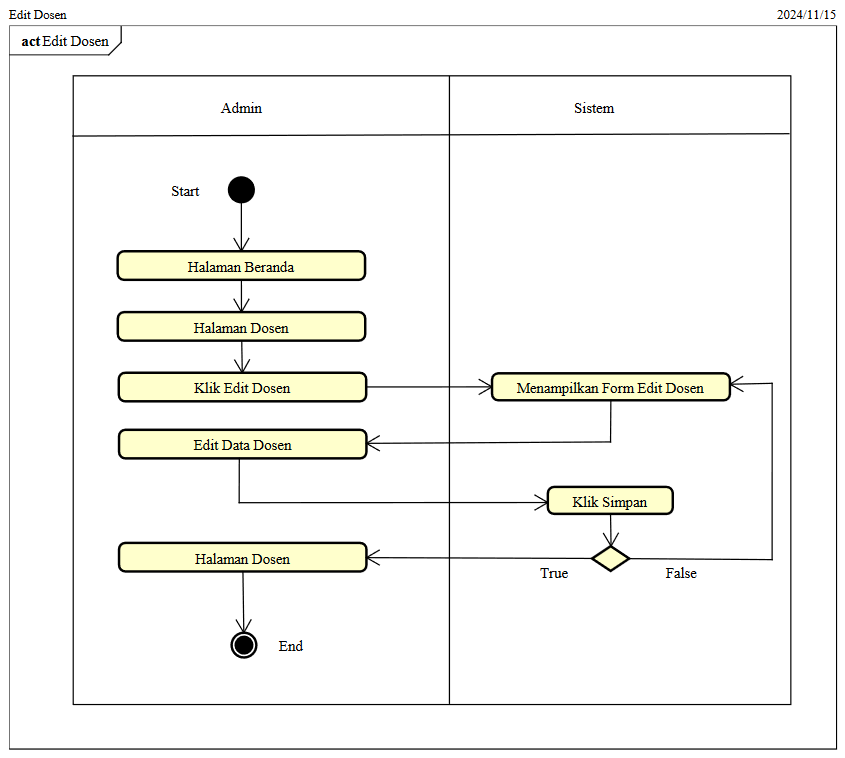
\includegraphics[width=0.82\textwidth]{konten/gambar/activity-diagram/edit-dosen.png}
	\caption{\textit{Activity Diagram} Edit Dosen}
	\label{activity-diagram-edit-dosen}
\end{figure}

\textit{Activity diagram} hapus dosen memberikan gambaran rinci tentang proses penghapusan dosen yang dilalui oleh pengguna. Diagram ini memandu langkah-langkah yang terlibat dalam proses penghapusan dosen, mulai dari pemilihan data dosen yang akan dihapus, konfirmasi oleh pengguna, hingga penghapusan data dosen dari sistem. \textit{Activity diagram} ini dapat dilihat pada Gambar \ref{activity-diagram-hapus-dosen}.
\begin{figure}
	\centering
	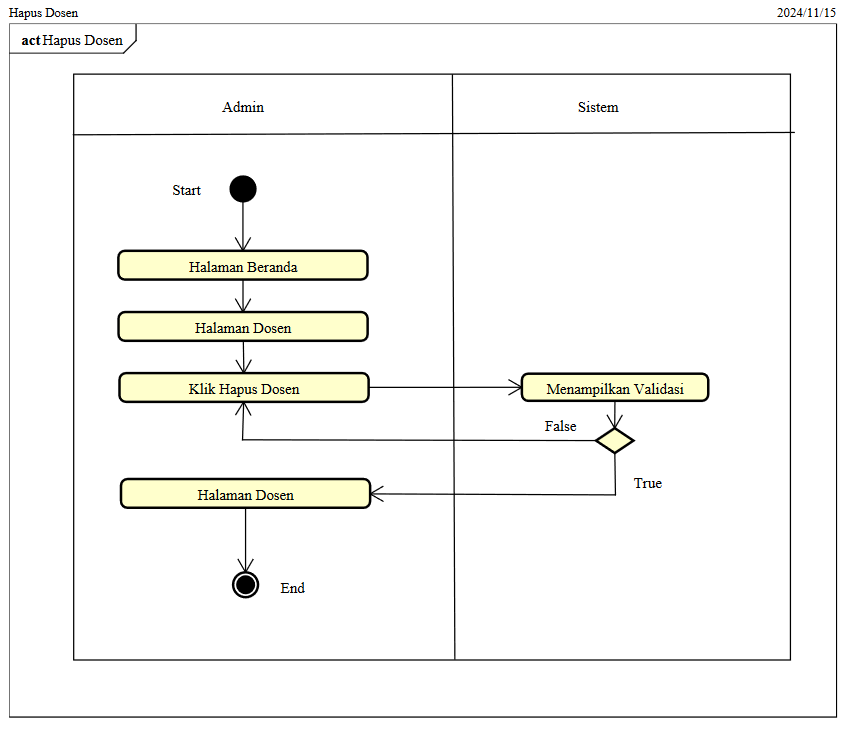
\includegraphics[width=0.82\textwidth]{konten/gambar/activity-diagram/hapus-dosen.png}
	\caption{\textit{Activity Diagram} Hapus Dosen}
	\label{activity-diagram-hapus-dosen}
\end{figure}

\textit{Activity diagram} tambah mata kuliah memberikan gambaran rinci tentang proses penambahan mata kuliah yang dilalui oleh pengguna. Diagram ini memandu langkah-langkah yang terlibat dalam proses penambahan mata kuliah, mulai dari input data oleh pengguna, validasi oleh sistem hingga penyimpanan data mata kuliah baru ke dalam sistem. \textit{Activity diagram} ini dapat dilihat pada Gambar \ref{activity-diagram-tambah-matkul}.
\begin{figure}
	\centering
	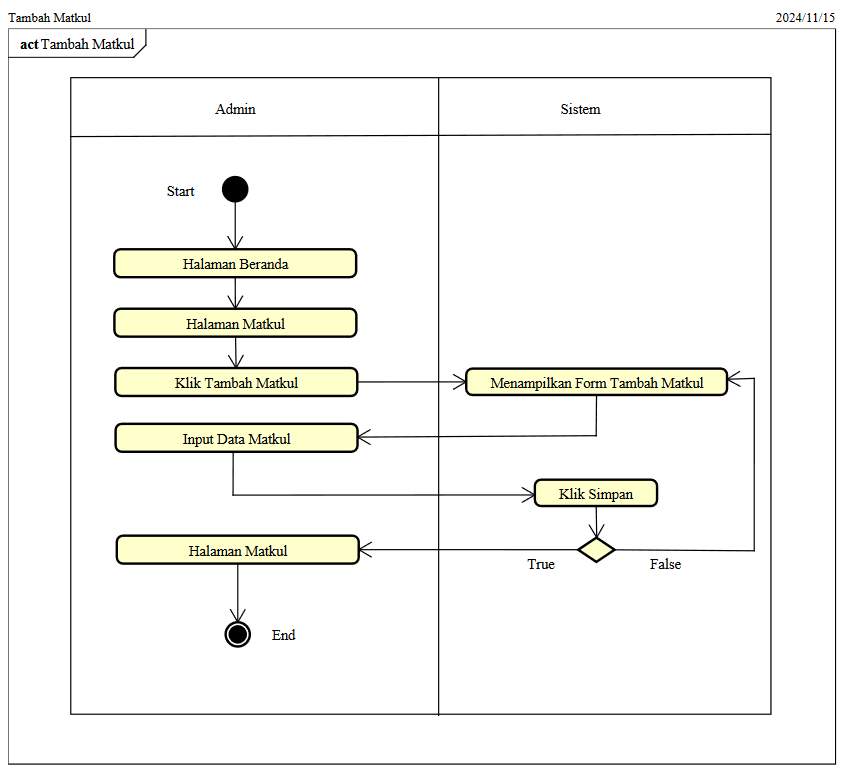
\includegraphics[width=0.82\textwidth]{konten/gambar/activity-diagram/tambah-matkul.png}
	\caption{\textit{Activity Diagram} Tambah Mata Kuliah}
	\label{activity-diagram-tambah-matkul}
\end{figure}

\textit{Activity diagram} edit mata kuliah memberikan gambaran rinci tentang proses pengeditan data mata kuliah yang dilalui oleh pengguna. Diagram ini memandu langkah-langkah yang terlibat dalam proses pengeditan mata kuliah, mulai dari pemilihan data mata kuliah yang akan diedit, input data baru oleh pengguna, validasi oleh sistem hingga penyimpanan data mata kuliah yang telah diperbarui ke dalam sistem. \textit{Activity diagram} ini dapat dilihat pada Gambar \ref{activity-diagram-edit-matkul}.
\begin{figure}
	\centering
	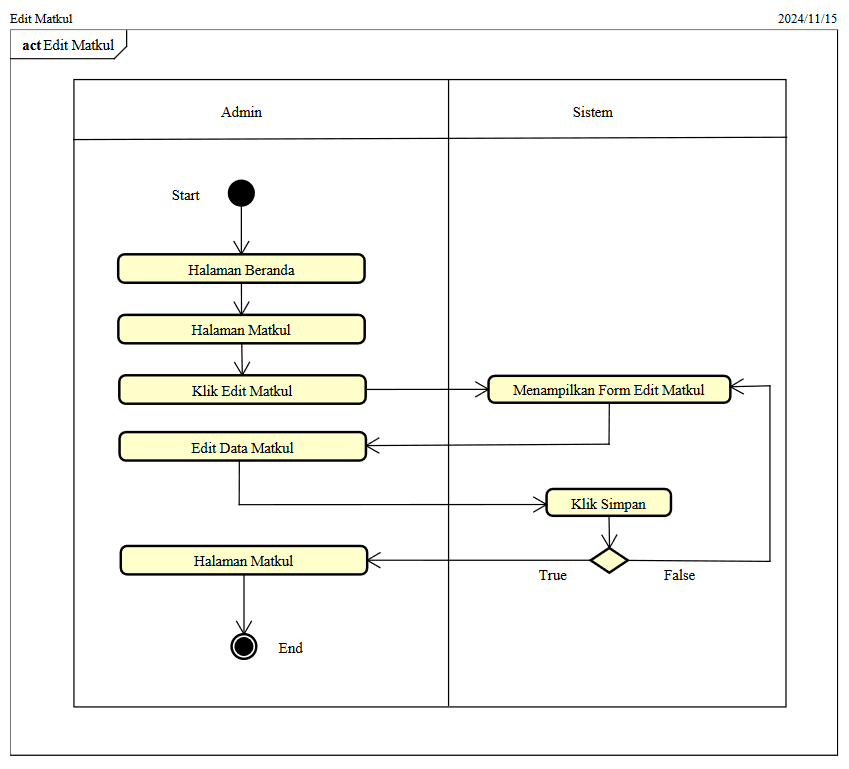
\includegraphics[width=0.82\textwidth]{konten/gambar/activity-diagram/edit-matkul.png}
	\caption{\textit{Activity Diagram} Edit Mata Kuliah}
	\label{activity-diagram-edit-matkul}
\end{figure}

\textit{Activity diagram} hapus mata kuliah memberikan gambaran rinci tentang proses penghapusan mata kuliah yang dilalui oleh pengguna. Diagram ini memandu langkah-langkah yang terlibat dalam proses penghapusan mata kuliah, mulai dari pemilihan data mata kuliah yang akan dihapus, konfirmasi oleh pengguna, hingga penghapusan data mata kuliah dari sistem. \textit{Activity diagram} ini dapat dilihat pada Gambar \ref{activity-diagram-hapus-matkul}.
\begin{figure}
	\centering
	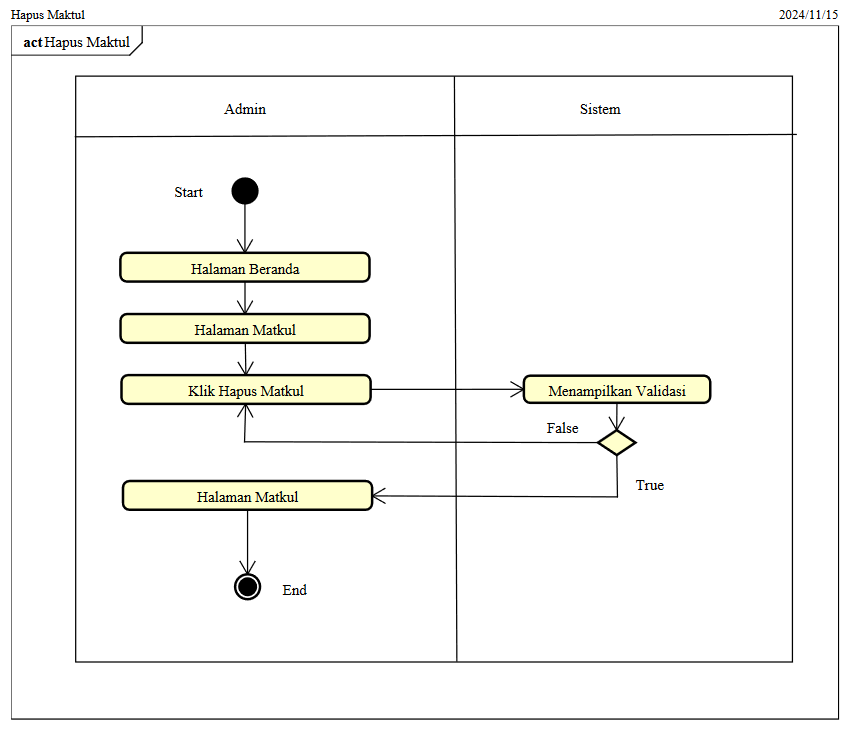
\includegraphics[width=0.82\textwidth]{konten/gambar/activity-diagram/hapus-matkul.png}
	\caption{\textit{Activity Diagram} Hapus Mata Kuliah}
	\label{activity-diagram-hapus-matkul}
\end{figure}

\textit{Activity diagram} tambah dosen memberikan gambaran rinci tentang proses penambahan dosen yang dilalui oleh pengguna. Diagram ini memandu langkah-langkah yang terlibat dalam proses penambahan dosen, mulai dari input data oleh pengguna, validasi oleh sistem hingga penyimpanan data dosen baru ke dalam sistem. \textit{Activity diagram} ini dapat dilihat pada Gambar \ref{activity-diagram-tambah-dosen}.
\begin{figure}
	\centering
	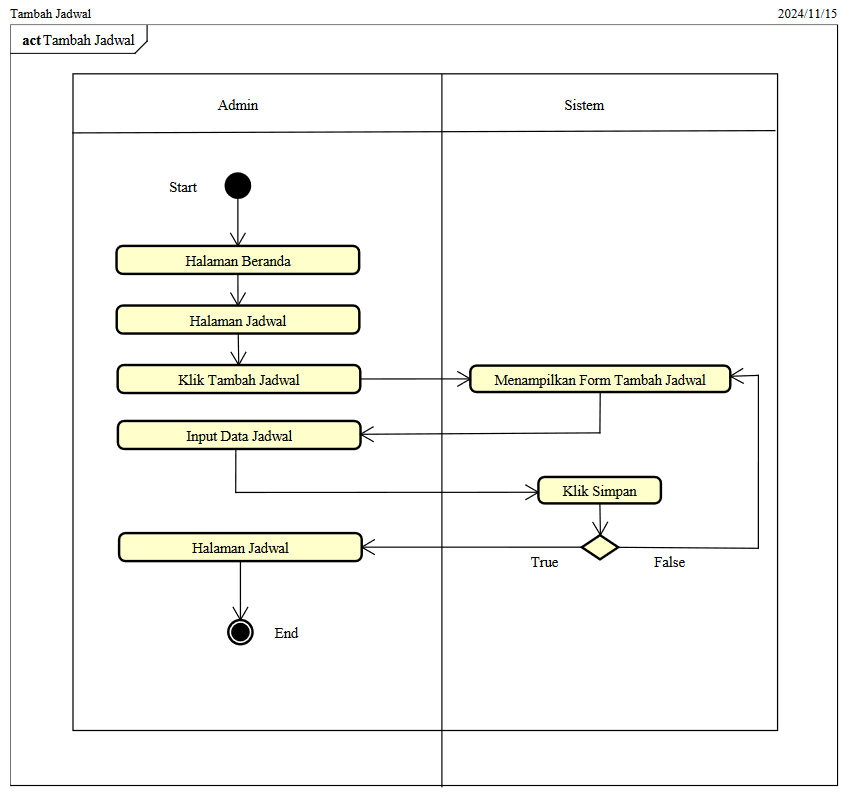
\includegraphics[width=0.82\textwidth]{konten/gambar/activity-diagram/tambah-jadwal.png}
	\caption{\textit{Activity Diagram} Tambah Jadwal}
	\label{activity-diagram-tambah-jadwal}
\end{figure}

\textit{Activity diagram} edit jadwal memberikan gambaran rinci tentang proses pengeditan jadwal yang dilalui oleh pengguna. Diagram ini memandu langkah-langkah yang terlibat dalam proses pengeditan jadwal, mulai dari pemilihan data jadwal yang akan diedit, input data baru oleh pengguna, validasi oleh sistem hingga penyimpanan data jadwal yang telah diperbarui ke dalam sistem. \textit{Activity diagram} ini dapat dilihat pada Gambar \ref{activity-diagram-edit-jadwal}.
\begin{figure}
	\centering
	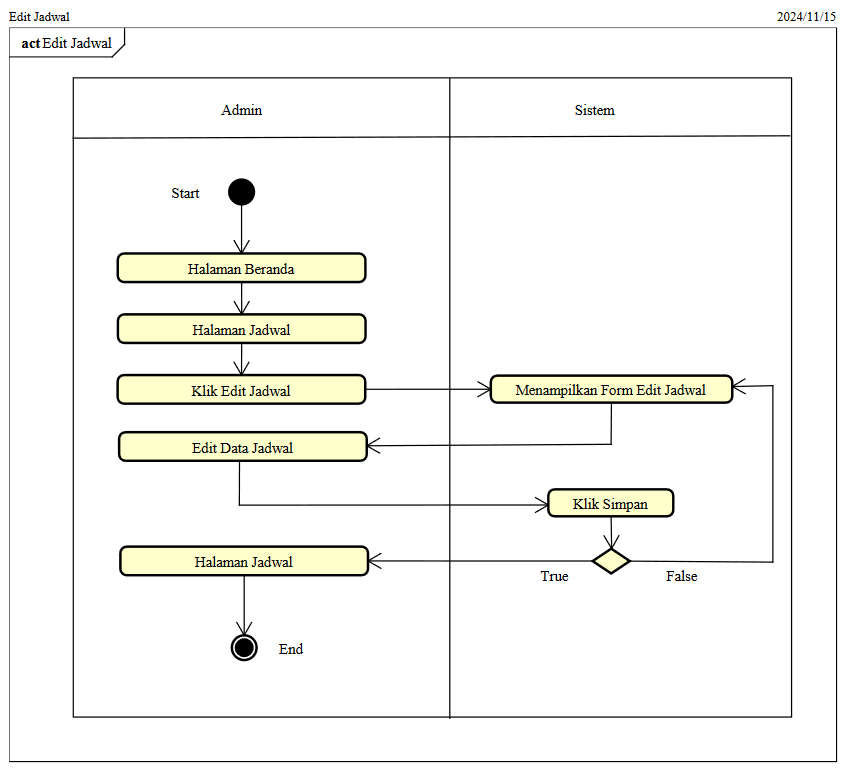
\includegraphics[width=0.82\textwidth]{konten/gambar/activity-diagram/edit-jadwal.png}
	\caption{\textit{Activity Diagram} Edit Jadwal}
	\label{activity-diagram-edit-jadwal}
\end{figure}

\textit{Activity diagram} hapus jadwal memberikan gambaran rinci tentang proses penghapusan jadwal yang dilalui oleh pengguna. Diagram ini memandu langkah-langkah yang terlibat dalam proses penghapusan jadwal, mulai dari pemilihan data jadwal yang akan dihapus, konfirmasi oleh pengguna, hingga penghapusan data jadwal dari sistem. \textit{Activity diagram} ini dapat dilihat pada Gambar \ref{activity-diagram-hapus-jadwal}.
\begin{figure}
	\centering
	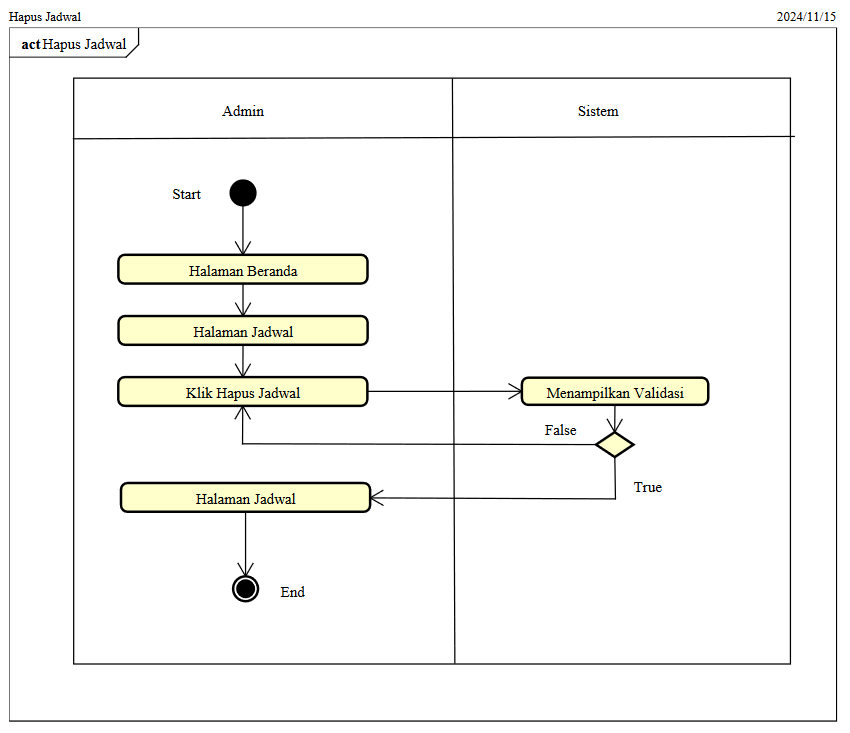
\includegraphics[width=0.82\textwidth]{konten/gambar/activity-diagram/hapus-jadwal.png}
	\caption{\textit{Activity Diagram} Hapus Jadwal}
	\label{activity-diagram-hapus-jadwal}
\end{figure}

% =======================================================================================================================
\subsection{\textit{Class Diagram}}
\textit{Class diagram} adalah representasi visual dari struktur kelas dalam sistem manajemen laboratorium, yang menunjukkan hubungan logis antar kelas. \textit{Class diagram} ini menyediakan deskripsi terperinci dari setiap kelas yang terlibat dalam sistem, termasuk atribut dan operasi yang diperlukan untuk mendukung fungsi manajemen laboratorium secara efektif. \textit{Class diagram} Sistem Informasi Manajemen Laboratorium dapat dilihat pada \pic~\ref{class-diagram}

\begin{figure}
	\centering
	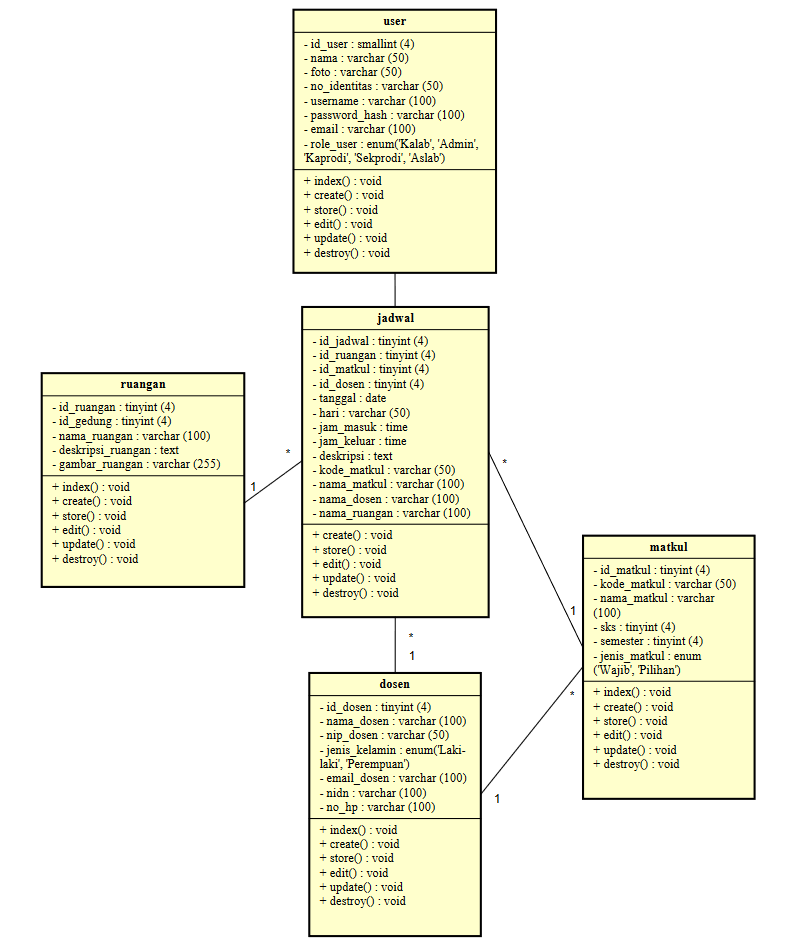
\includegraphics[width=0.82\textwidth]{konten/gambar/class-diagram.png}
	\caption{\textit{Class Diagram} Sistem Manajemen Laboratorium}
	\label{class-diagram}
\end{figure}

Relasi antara jadwal dengan ruangan, dosen, dan mata kuliah diwakili oleh id\_ruangan, id\_dosen, dan id\_matkul pada jadwal. Id\_ruangan menunjukkan keterkaitan jadwal dengan ruangan tertentu, id\_dosen menunjukkan keterkaitan jadwal dengan dosen tertentu, dan id\_matkul menunjukkan keterkaitan jadwal dengan mata kuliah tertentu. Hubungan ini digambarkan dengan garis yang menghubungkan entitas jadwal ke masing-masing entitas ruangan, dosen, dan mata kuliah dalam diagram.

% =======================================================================================================================
\subsection{Perancangan \text{Database}}
Perancangan \textit{database} adalah perancangan basis data yang akan digunakan pada sebuah sistem, didasari oleh data perusahaan. Perancangan ini bertujuan agar tiap field data yang memiliki relasi dapat terhubung pada tabel di \textit{database}, sehingga proses pengaksesan data akan dapat telaksana dengan lebih baik. Berikut adalah detail perancangan serta relasi yang ada pada \textit{database} sistem informasi inventaris laboratorium pada Laboratorium Sistem Informasi. Berikut tabel perancangan \textit{database}:

\begin{enumerate}

	\item Perancangan \textit{Database} Tabel Dosen \\
	      \begin{tabular}{lll}
		      Nama \textit{Database} & : & man\_lab  \\
		      Nama Tabel             & : & dosen     \\
		      Field Kunci            & : & id\_dosen \\
	      \end{tabular}

	      Tabel Dosen dirancang untuk menyimpan informasi komprehensif tentang staf pengajar. Struktur tabel ini mencakup berbagai atribut yang diperlukan untuk mengidentifikasi dan mengelola data dosen secara efisien. Berikut adalah penjelasan ilmiah mengenai struktur dan fungsi tabel Dosen:

	      \begin{itemize}
		      \item Tabel ini menetapkan \textit{id\_dosen} sebagai kunci utama dengan tipe data tinyint(4) dan fitur \textit{auto increment}, yang memastikan bahwa setiap dosen diberikan identifikasi yang unik dalam sistem.
		      \item Atribut 'nama\_dosen' dan 'nip\_dosen' berfungsi untuk menyimpan informasi dasar tentang dosen, yang memudahkan pengenalan personal dalam lingkungan akademis.
		      \item Field 'jenis\_kelamin' memakai tipe data enum untuk menjaga konsistensi data dan membantu dalam analisis demografis.
		      \item 'email\_dosen' dan 'no\_hp' merupakan saluran komunikasi yang vital, yang memungkinkan komunikasi yang efektif antara dosen dan sistem.
		      \item Atribut 'nidn' (Nomor Induk Dosen Nasional) mencatat identifikasi nasional yang unik untuk dosen, yang mendukung integrasi dengan sistem pendidikan tinggi yang lebih luas.
	      \end{itemize}

	      Struktur tabel ini dirancang dengan mempertimbangkan kebutuhan manajemen data dosen yang komprehensif, efisiensi penyimpanan, dan kemudahan dalam pemrosesan dan analisis data.

		      {
			      \fontsize{10}{12}\selectfont
			      \begin{longtable}{l l l l}
				      \caption{Tabel Dosen}
				      \label{admin}                                                                                         \\
				      \hline
				      \textbf{\textit{Field}} & \textbf{\textit{Type}} & \textbf{\textit{Length}}   & \textbf{\textit{Key}} \\
				      \hline
				      \endfirsthead

				      \multicolumn{4}{c}{\tablename\ \thetable\ {Tabel Dosen} \space (Tabel lanjutan...)}                   \\
				      \hline
				      \textbf{\textit{Field}} & \textbf{\textit{Type}} & \textbf{\textit{Length}}   & \textbf{\textit{Key}} \\
				      \hline
				      \endhead

				      id\_dosen               & tinyint                & 4                          & Primary key (A\_I)    \\
				      nama\_dosen             & varchar                & 100                        &                       \\
				      nip\_dosen              & varchar                & 50                         &                       \\
				      jenis\_kelamin          & enum                   & ('Laki-laki', 'Perempuan') &                       \\
				      email\_dosen            & varchar                & 100                        &                       \\
				      nidn                    & varchar                & 100                        &                       \\
				      no\_hp                  & varchar                & 100                        &                       \\
				      \hline
			      \end{longtable}
		      }

	\item Perancangan \textit{Database} Tabel Matkul \\
	      \begin{tabular}{lll}
		      Nama \textit{Database} & : & man\_lab   \\
		      Nama Tabel             & : & matkul     \\
		      Field Kunci            & : & id\_matkul \\
	      \end{tabular}

	      Tabel Matkul dirancang untuk menyimpan informasi tentang mata kuliah yang ditawarkan dalam program akademik. Struktur tabel ini mencakup berbagai atribut yang diperlukan untuk mengidentifikasi dan mengelola data mata kuliah secara efisien. Berikut adalah penjelasan ilmiah mengenai struktur dan fungsi tabel Matkul:

	      \begin{itemize}
		      \item Tabel ini memanfaatkan \textit{id\_matkul} sebagai kunci utama dengan tipe data tinyint(4) dan fitur \textit{auto increment}, yang menjamin bahwa setiap mata kuliah diberi identifikasi yang unik di dalam sistem.
		      \item Atribut 'kode\_matkul' dan 'nama\_matkul' berfungsi untuk menyimpan informasi dasar yang membantu dalam mengenali mata kuliah dengan cepat di lingkungan akademik.
		      \item Field 'sks' dan 'semester' berisi informasi krusial mengenai bobot akademik dan penjadwalan mata kuliah dalam kurikulum, yang penting untuk perencanaan pendidikan.
		      \item Atribut 'jenis\_matkul' memakai tipe data enum untuk membedakan mata kuliah menjadi kategori wajib atau pilihan, mendukung kelancaran dalam pengelolaan kurikulum.
	      \end{itemize}

	      Struktur tabel ini dirancang dengan mempertimbangkan kebutuhan manajemen data mata kuliah yang komprehensif, efisiensi penyimpanan, dan kemudahan dalam pemrosesan dan analisis data kurikulum.

		      {
			      \fontsize{10}{12}\selectfont
			      \begin{longtable}{l l l l}
				      \caption{Tabel Matkul}
				      \label{admin}                                                                                       \\
				      \hline
				      \textbf{\textit{Field}} & \textbf{\textit{Type}} & \textbf{\textit{Length}} & \textbf{\textit{Key}} \\
				      \hline
				      \endfirsthead

				      \multicolumn{4}{c}{\tablename\ \thetable\ {Tabel Matkul} \space (Tabel lanjutan...)}                \\
				      \hline
				      \textbf{\textit{Field}} & \textbf{\textit{Type}} & \textbf{\textit{Length}} & \textbf{\textit{Key}} \\
				      \hline
				      \endhead

				      id\_matkul              & tinyint                & 4                        & Primary key (A\_I)    \\
				      kode\_matkul            & varchar                & 50                       &                       \\
				      nama\_matkul            & varchar                & 100                      &                       \\
				      sks                     & tinyint                & 4                        &                       \\
				      semester                & tinyint                & 4                        &                       \\
				      jenis\_matkul           & enum                   & ('Wajib', 'Pilihan')     &                       \\
				      \hline
			      \end{longtable}
		      }

	\item Perancangan \textit{Database} Tabel Ruangan \\
	      \begin{tabular}{lll}
		      Nama \textit{Database} & : & man\_lab    \\
		      Nama Tabel             & : & ruangan     \\
		      Field Kunci            & : & id\_ruangan \\
	      \end{tabular}

	      Tabel Ruangan dirancang untuk menyimpan informasi tentang ruangan-ruangan yang tersedia untuk kegiatan akademik. Struktur tabel ini mencakup berbagai atribut yang diperlukan untuk mengidentifikasi dan mengelola data ruangan secara efisien. Berikut adalah penjelasan ilmiah mengenai struktur dan fungsi tabel Ruangan:

	      \begin{itemize}
		      \item Tabel ini memanfaatkan \textit{id\_ruangan} sebagai \textit{primary key}. Dengan menggunakan tipe data tinyint(4) dan fitur \textit{auto increment}, tabel ini memastikan bahwa setiap ruangan tercatat dengan identitas uniknya sendiri dalam sistem.
		      \item Atribut 'id\_gedung' bertindak sebagai \textit{foreign key} yang mengaitkan setiap ruangan dengan gedungnya, membantu dalam mengatur lokasi dengan lebih terstruktur.
		      \item Field 'nama\_ruangan' berisi nama yang memudahkan pengguna dalam mengenali setiap ruangan.
		      \item Atribut 'deskripsi\_ruangan' memberikan ruang untuk menambahkan keterangan lebih lanjut mengenai fasilitas atau ciri khas dari ruangan tersebut.
		      \item Field 'gambar\_ruangan' berisi jalur ke file gambar yang berkaitan dengan ruangan, memudahkan dalam visualisasi dan lebih memahami penampilan ruangan tersebut.
	      \end{itemize}

	      Struktur tabel ini dirancang dengan mempertimbangkan kebutuhan manajemen data ruangan yang komprehensif, efisiensi penyimpanan, dan kemudahan dalam pemrosesan dan analisis data fasilitas.

		      {
			      \fontsize{10}{12}\selectfont
			      \begin{longtable}{l l l l}
				      \caption{Tabel Ruangan}
				      \label{admin}                                                                                       \\
				      \hline
				      \textbf{\textit{Field}} & \textbf{\textit{Type}} & \textbf{\textit{Length}} & \textbf{\textit{Key}} \\
				      \hline
				      \endfirsthead

				      \multicolumn{4}{c}{\tablename\ \thetable\ {Tabel Ruangan} \space (Tabel lanjutan...)}               \\
				      \hline
				      \textbf{\textit{Field}} & \textbf{\textit{Type}} & \textbf{\textit{Length}} & \textbf{\textit{Key}} \\
				      \
				      \endhead

				      id\_ruangan             & tinyint                & 4                        & Primary key (A\_I)    \\
				      id\_gedung              & tinyint                & 4                        & Foreign key           \\
				      nama\_ruangan           & varchar                & 100                      &                       \\
				      deskripsi\_ruangan      & text                   &                          &                       \\
				      gambar\_ruangan         & varchar                & 255                      &                       \\
				      \hline
			      \end{longtable}
		      }

	\item Perancangan \textit{Database} Tabel Jadwal \\
	      \begin{tabular}{lll}
		      Nama \textit{Database} & : & man\_lab   \\
		      Nama Tabel             & : & jadwal     \\
		      Field Kunci            & : & id\_jadwal \\
	      \end{tabular}

	      Tabel Jadwal dirancang untuk menyimpan informasi tentang penjadwalan kegiatan akademik. Struktur tabel ini mencakup berbagai atribut yang diperlukan untuk mengidentifikasi dan mengelola data jadwal secara efisien. Berikut adalah penjelasan ilmiah mengenai struktur dan fungsi tabel Jadwal:

	      \begin{itemize}
		      \item Tabel ini dilengkapi dengan \textit{id\_jadwal} sebagai \textit{primary key}. Dengan tipe data tinyint(4) dan fitur \textit{auto increment}, setiap jadwal dijamin memiliki identifikasi yang unik dalam sistem.
		      \item Atribut seperti 'id\_ruangan', 'id\_matkul', dan 'id\_dosen' bertindak sebagai \textit{foreign key}, yang mengaitkan jadwal dengan informasi tentang ruangan, mata kuliah, dan dosen yang relevan, sehingga memudahkan pengelolaan jadwal secara terpadu.
		      \item Field seperti 'tanggal', 'hari', 'jam\_masuk', dan 'jam\_keluar' berperan penting dalam mencatat waktu spesifik untuk setiap kegiatan dalam jadwal.
		      \item Atribut 'deskripsi' memberikan ruang untuk menambahkan informasi detail tentang kegiatan atau jadwal yang direncanakan.
		      \item Field-field seperti 'kode\_matkul', 'nama\_matkul', 'nama\_dosen', dan 'nama\_ruangan' walaupun redundan, tetapi sangat membantu dalam mempercepat akses informasi tanpa perlu menggabungkan tabel berulang kali.
	      \end{itemize}

	      Struktur tabel ini dirancang dengan mempertimbangkan kebutuhan manajemen data jadwal yang komprehensif, efisiensi dalam pengambilan data, dan fleksibilitas dalam pengelolaan jadwal akademik.

		      {
			      \fontsize{10}{12}\selectfont
			      \begin{longtable}{l l l l}
				      \caption{Tabel Jadwal}
				      \label{admin}                                                                                       \\
				      \hline
				      \textbf{\textit{Field}} & \textbf{\textit{Type}} & \textbf{\textit{Length}} & \textbf{\textit{Key}} \\
				      \hline
				      \endfirsthead

				      \multicolumn{4}{c}{\tablename\ \thetable\ {Tabel Jadwal} \space (Tabel lanjutan...)}                \\
				      \hline
				      \textbf{\textit{Field}} & \textbf{\textit{Type}} & \textbf{\textit{Length}} & \textbf{\textit{Key}} \\
				      \hline
				      \endhead

				      id\_jadwal              & tinyint                & 4                        & Primary key (A\_I)    \\
				      id\_ruangan             & tinyint                & 4                        & Foreign key           \\
				      id\_matkul              & varchar                & 4                        & Foreign key           \\
				      id\_dosen               & varchar                & 4                        & Foreign key           \\
				      tanggal                 & date                   &                          &                       \\
				      hari                    & varchar                & 50                       &                       \\
				      jam\_masuk              & time                   &                          &                       \\
				      jam\_keluar             & time                   &                          &                       \\
				      deskripsi               & text                   &                          &                       \\
				      kode\_matkul            & tinyint                & 4                        &                       \\
				      nama\_matkul            & varchar                & 100                      &                       \\
				      nama\_dosen             & varchar                & 100                      &                       \\
				      nama\_ruangan           & varchar                & 100                      &                       \\
				      \hline
			      \end{longtable}
		      }

	\item Perancangan \textit{Database} Tabel \textit{User} \\
	      \begin{tabular}{lll}
		      Nama \textit{Database} & : & man\_lab          \\
		      Nama Tabel             & : & \textit{user}     \\
		      Field Kunci            & : & id\_\textit{user} \\
	      \end{tabular}

	      Tabel \textit{User} dirancang untuk menyimpan informasi pengguna dalam sistem manajemen laboratorium. Struktur tabel ini mencakup berbagai atribut yang diperlukan untuk mengidentifikasi dan mengautentikasi pengguna, serta mengelola hak akses mereka. Berikut adalah penjelasan ilmiah mengenai struktur dan fungsi tabel \textit{User}:

	      \begin{itemize}
		      \item Tabel ini memberikan setiap pengguna identifikasi unik melalui \textit{id\_user} yang bertindak sebagai \textit{primary key}. Tipe data yang digunakan adalah smallint(4) dengan fitur \textit{auto increment}.
		      \item Atribut 'nama' dan 'no\_identitas' berfungsi untuk menyimpan informasi dasar tentang pengguna, sehingga memudahkan pengenalan personal dalam lingkup organisasi.
		      \item Field 'foto' berisi lokasi penyimpanan file gambar profil pengguna, yang membantu dalam personalisasi tampilan antarmuka pengguna.
		      \item \textit{Username} dan \textit{password\_hash} digunakan sebagai kredensial untuk masuk ke sistem, dengan \textit{password} yang telah dienkripsi guna menjaga keamanan data.
		      \item Atribut 'role\_user' dengan tipe data enum digunakan untuk menentukan peran pengguna dalam sistem, yang mendukung pengelolaan hak akses secara efektif.
	      \end{itemize}

	      Struktur tabel ini dirancang dengan mempertimbangkan aspek keamanan, efisiensi penyimpanan data, dan fleksibilitas dalam pengelolaan pengguna sistem.

		      {
			      \fontsize{10}{12}\selectfont
			      \begin{longtable}{l l l l}
				      \caption{Tabel \textit{User}}
				      \label{admin}                                                                                                                 \\
				      \hline
				      \textbf{\textit{Field}} & \textbf{\textit{Type}} & \textbf{\textit{Length}}                           & \textbf{\textit{Key}} \\
				      \hline
				      \endfirsthead

				      \multicolumn{4}{c}{\tablename\ \thetable\ {Tabel \textit{User}} \space (Tabel lanjutan...)}                                   \\
				      \hline
				      \textbf{\textit{Field}} & \textbf{\textit{Type}} & \textbf{\textit{Length}}                           & \textbf{\textit{Key}} \\
				      \hline
				      \endhead

				      id\_\textit{user}       & smallint               & 4                                                  & Primary key (A\_I)    \\
				      nama                    & varchar                & 50                                                 &                       \\
				      foto                    & varchar                & 50                                                 &                       \\
				      no\_identitas           & varchar                & 50                                                 &                       \\
				      \textit{username}       & varchar                & 100                                                &                       \\
				      \textit{password}\_hash & varchar                & 100                                                &                       \\
				      role\_\textit{user}     & enum                   & ('Admin', 'Kalab', 'Kaprodi', 'Sekprodi', 'Aslab') &                       \\
				      \hline
			      \end{longtable}
		      }

\end{enumerate}

% =======================================================================================================================
\subsection{Perancangan Struktur Menu}
Perancangan menu sistem informasi manajemen inventaris laboratorium dibagi menjadi 5 tingkatan hak akses sesuai kewenangan pengguna. Setiap pengguna dapat mengakses fitur sesuai peran dan tanggung jawab mereka.

Menu Admin, sebagai tingkat akses tertinggi, memiliki wewenang penuh untuk mengelola semua fitur, termasuk pendanaan, manajemen barang, penjadwalan, dll. Kepala Laboratorium (Kalab) memiliki akses hampir sama dengan Admin, tetapi dengan beberapa pembatasan. Kalab dapat mengelola pendanaan, barang, jadwal, dan data dosen serta mata kuliah. Ketua Program Studi (Kaprodi) dan Sekretaris Program Studi (Sekprodi) fokus pada pengawasan dan monitoring, dengan akses ke fitur pendanaan, manajemen barang, dan dokumentasi. Asisten Laboratorium (Aslab) memiliki akses untuk mendukung operasional harian termasuk pengelolaan barang, dan pemeliharaan peralatan laboratorium.

Struktur menu yang terorganisir ini dirancang untuk memudahkan pengelolaan inventaris laboratorium secara sistematis dan terkontrol. Setiap tingkatan pengguna memiliki batasan akses yang jelas, yang membantu dalam menjaga keamanan dan integritas data sistem. Perancangan menu ini menjadi landasan penting dalam pengembangan antarmuka pengguna dan implementasi berbagai fungsi sistem yang akan dibahas lebih lanjut pada bagian berikutnya. Dengan struktur menu yang terorganisir ini, diharapkan pengelolaan inventaris laboratorium dapat berjalan lebih efisien dan terkoordinasi dengan baik antar berbagai tingkatan pengguna. Gambar struktur menu ini dapat dilihat pada \pic~\ref{StrukturMenuILMIS}

\begin{figure}
	\centering
	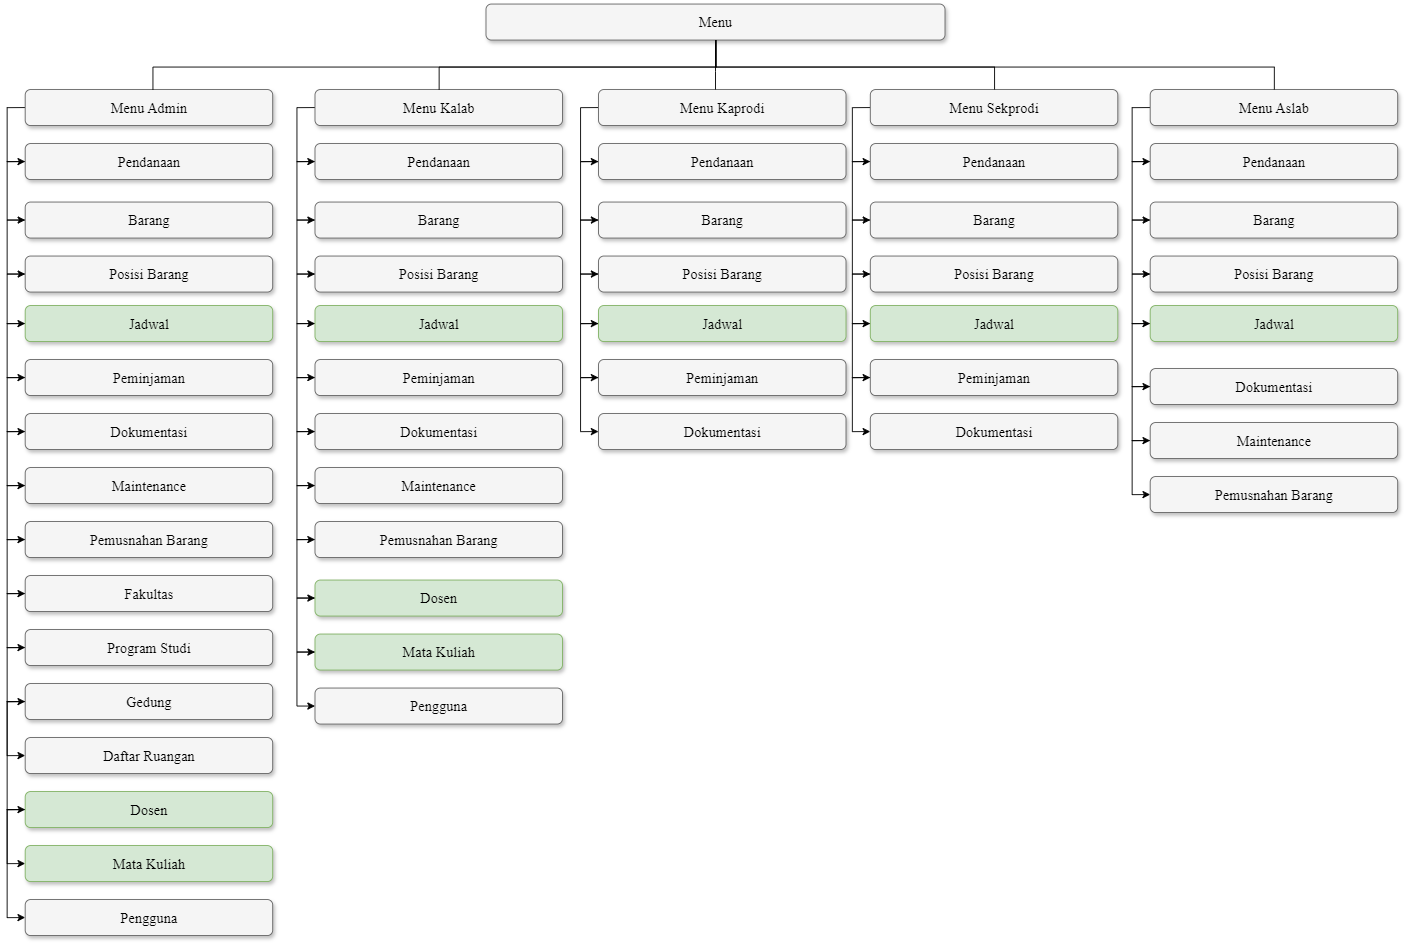
\includegraphics[width=0.82\textwidth]{konten/gambar/menu.png}
	\caption{Struktur Menu Sistem Manajemen Laboratorium}
	\label{StrukturMenuILMIS}
\end{figure}

Pengembangan sistem ini menambahkan fitur baru yang ditandai dengan warna hijau pada struktur menu, termasuk fitur Jadwal untuk semua level pengguna (Admin, Kalab, Kaprodi, Sekprodi, dan Aslab) serta fitur Dosen dan Mata Kuliah yang kini dapat diakses oleh Kalab. Penambahan ini bertujuan untuk meningkatkan pengelolaan laboratorium dan efisiensi koordinasi antara pengelola dan dosen.

% =======================================================================================================================
\subsection{Perancangan \textit{Interface}}
Perancangan \textit{interface} berfungsi untuk menjelaskan tentang desain program sistem informasi manajemen laboratorium yang akan dibangun. Hal ini dilakukan untuk mempermudah pengguna dalam mengetahui proses yang terdapat pada sistem informasi manajemen laboratorium tersebut.

\begin{enumerate}
	\item Rancangan tampilan \textit{landing page} yang berfungsi sebagai halaman pertama untuk sistem informasi manajemen laboratorium dapat dilihat pada \pic~\ref{fig:kelola-jadwal-1}
	      \begin{figure}
		      \centering
		      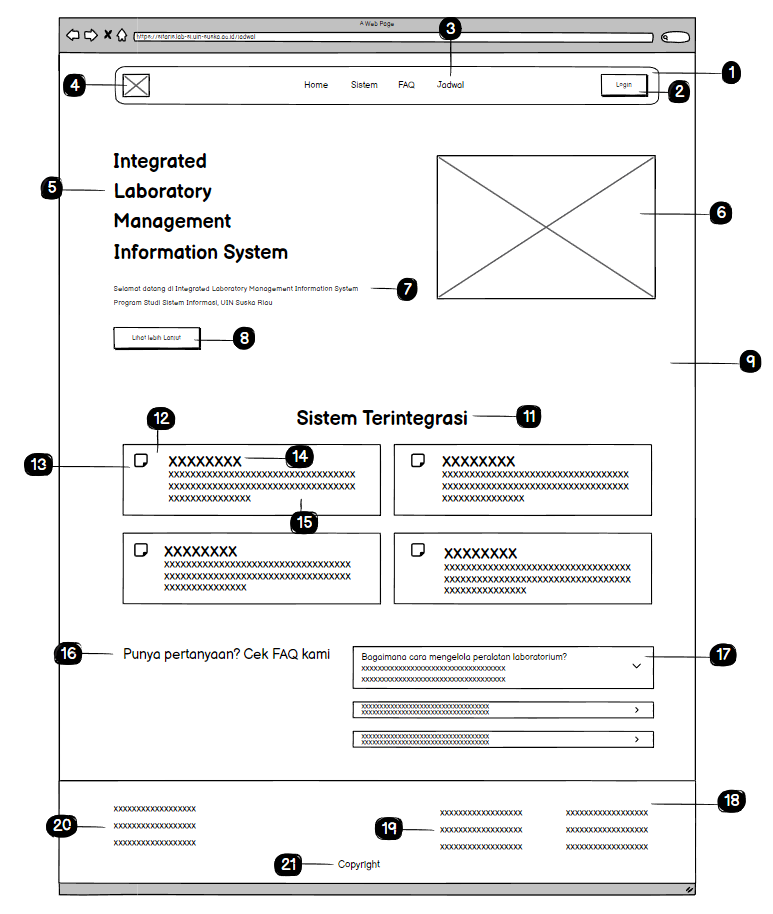
\includegraphics[width=0.82\textwidth]{konten/gambar/landing-page.png}
		      \caption{Tampilan Halaman Utama Sistem Manajemen Laboratorium}
		      \label{fig:kelola-jadwal-1}
	      \end{figure}

	      \begin{longtable}{|c|p{0.55\textwidth}|}
		      \caption{Tabel Keterangan Tampilan Halaman Utama Sistem Manajemen Laboratorium}                                                                 \\
		      \hline
		      \textbf{Nomor Callouts} & \textbf{Keterangan}                                                                                                   \\
		      \hline
		      \endfirsthead

		      \multicolumn{2}{c}{{\textit{Lanjutan dari halaman sebelumnya...}}}                                                                              \\
		      \hline
		      \textbf{Nomor Callouts} & \textbf{Keterangan}                                                                                                   \\
		      \hline
		      \endhead

		      \hline \multicolumn{2}{|r|}{{\textit{Bersambung ke halaman berikutnya...}}}                                                                     \\
		      \endfoot

		      \hline
		      \endlastfoot

		      1                       & Browser toolbar dengan width: 100\%, height: 40px, background-color: \#FFFFFF                                         \\
		      2                       & Logo berukuran width: 40px, height: 40px, dengan margin-left: 24px pada pojok kiri atas                               \\
		      3                       & Navigation menu menggunakan font-family: Poppins, font-size: 14px, dengan gap: 32px antar menu                        \\
		      4                       & Button Login dengan padding: 8px 16px, border-radius: 6px, background-color: \#2563EB                                 \\
		      5                       & Container header dengan width: 100\%, height: 64px, box-shadow: 0 1px 3px rgba(0,0,0,0.1)                             \\
		      6                       & Text "Integrated Laboratory" menggunakan font-family: Poppins, font-size: 48px, font-weight: 600, margin-bottom: 16px \\
		      7                       & Text "Management Information System" berwarna \#2563EB dengan font-weight: 600                                        \\
		      8                       & Button "Lihat Lebih Lanjut" dengan padding: 12px 24px, background-color: \#2563EB                                     \\
		      9                       & Container image dengan width: 560px, height: 400px, border-radius: 8px                                                \\
		      10                      & Container content dengan max-width: 560px dan margin-right: 64px                                                      \\
		      11                      & Heading "Sistem Terintegrasi" dengan text-align: center, font-size: 36px, margin: 64px 0 32px                         \\
		      12                      & Container cards dengan display: grid, grid-template-columns: repeat(2, 1fr), gap: 24px                                \\
		      13                      & Card pertama dengan padding: 24px, background: white, border-radius: 8px, box-shadow: 0 1px 3px rgba(0,0,0,0.1)       \\
		      14                      & Text content pada card dengan font-size: 14px, line-height: 1.6, color: \#374151                                      \\
		      15                      & Card kedua dengan styling sama seperti card pertama                                                                   \\
		      16                      & Card ketiga dengan styling sama seperti card pertama                                                                  \\
		      17                      & Section FAQ dengan max-width: 800px, margin: 64px auto                                                                \\
		      18                      & Container question dengan padding: 24px, border-bottom: 1px solid \#E5E7EB                                            \\
		      19                      & Footer section dengan background: \#1E293B, padding: 64px 24px                                                        \\
		      20                      & Copyright text dengan font-size: 14px, color: \#9CA3AF                                                                \\
		      21                      & Footer links dengan display: flex, gap: 32px, margin-top: 32px                                                        \\
	      \end{longtable}

	\item Rancangan tampilan pilih aplikasi untuk login dapat dilihat pada \pic~\ref{fig:kelola-jadwal-2}
	      \begin{figure}
		      \centering
		      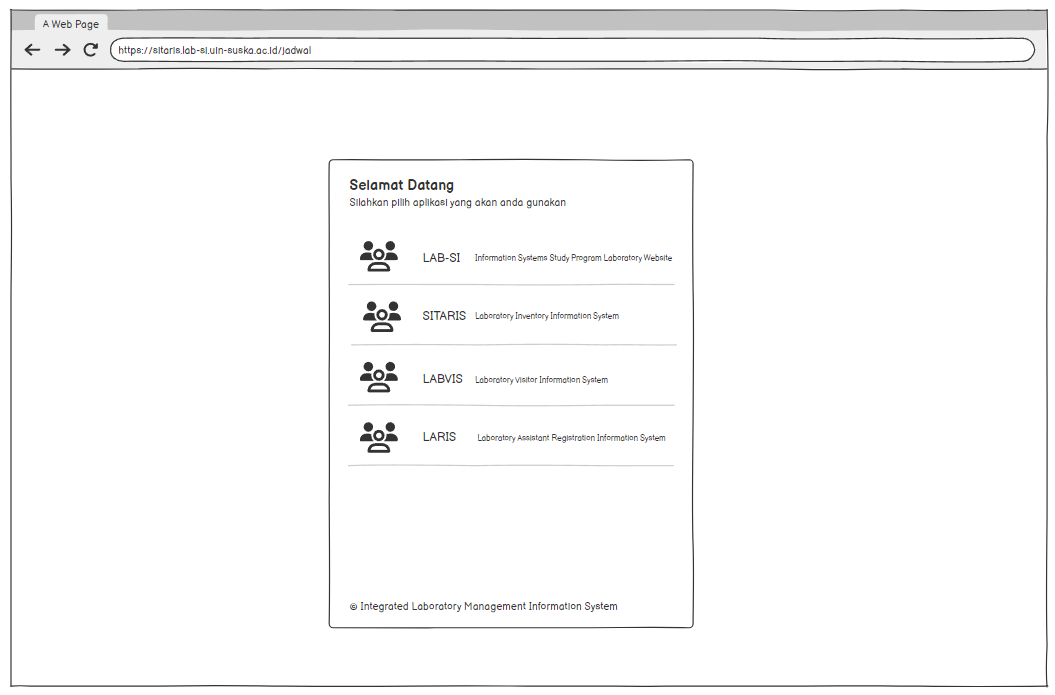
\includegraphics[width=0.82\textwidth]{konten/gambar/pilih-login.png}
		      \caption{Tampilan Pilihan Login untuk Sistem Manajemen Laboratorium}
		      \label{fig:kelola-jadwal-2}
	      \end{figure}

	      \begin{table}[H]
		      \centering
		      \caption{Tabel Keterangan Tampilan Halaman Selamat Datang}
		      \begin{tabular}{|c|p{0.55\textwidth}|}
			      \hline
			      \textbf{Nomor Callouts} & \textbf{Keterangan}                                                                          \\
			      \hline
			      1                       & Text header "Selamat Datang" dengan fonts Poppins, warna font \#73879C                       \\
			      2                       & Text sub-header "Silahkan pilih aplikasi yang akan anda gunakan" dengan fonts Helvetica Neue \\
			      3                       & Container card dengan background color \#FFFFFF dan border-radius 8px                        \\
			      4                       & Link ILMIS dengan icon users dan text "Integrated Laboratory Management Information System"  \\
			      5                       & Link LABVIS dengan icon users dan text "Laboratory Visitor Information System"               \\
			      6                       & Link LARIS dengan icon users dan text "Laboratory Assistant Registration Information System" \\
			      \hline
		      \end{tabular}
	      \end{table}

	\item Rancangan tampilan kelola jadwal yang berfungsi untuk mengelola jadwal laboratorium dapat dilihat pada \pic~\ref{fig:jadwal}
	      \begin{figure}
		      \centering
		      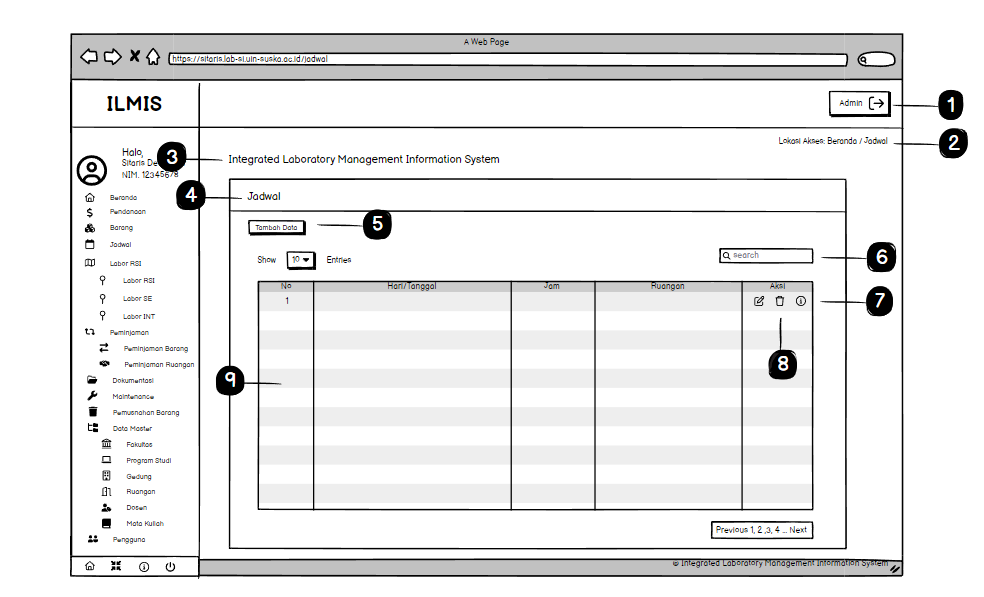
\includegraphics[width=0.82\textwidth]{konten/gambar/user interface/ui-jadwal.png}
		      \caption{Tampilan Kelola Jadwal Laboratorium}
		      \label{fig:jadwal}
	      \end{figure}

	      \begin{table}[H]
		      \centering
		      \caption{Tabel Keterangan Tampilan Kelola Jadwal}
		      \begin{tabular}{|c|p{0.55\textwidth}|}
			      \hline
			      \textbf{Nomor Callouts} & \textbf{Keterangan}                                             \\
			      \hline
			      1                       & Button "Admin" dengan icon arrow-right di pojok kanan atas      \\
			      2                       & Text "Logout Aktif: Beranda / Jadwal" dengan alignment right    \\
			      3                       & Profile section dengan nama user "NIM: 1234567" dan foto profil \\
			      4                       & Text header "Jadwal" dengan fonts Helvetica Neue                \\
			      5                       & Button "Tambah Data" dengan warna primary (\#2563EB)            \\
			      6                       & Search input field dengan icon search di sebelah kanan          \\
			      7                       & Action buttons (edit, delete, info) di kolom Aksi               \\
			      8                       & Data table dengan kolom: No, Hari/Tanggal, Jam, Ruangan, Aksi   \\
			      9                       & Sidebar menu dengan icons dan text untuk navigasi sistem        \\
			      \hline
		      \end{tabular}
	      \end{table}

	      \begin{figure}
		      \centering
		      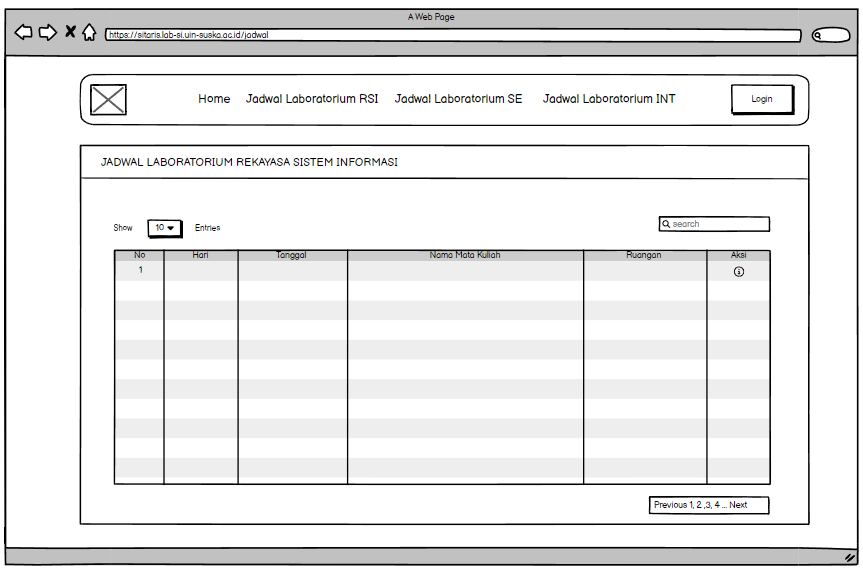
\includegraphics[width=0.82\textwidth]{konten/gambar/user interface/ui-jadwal-rsi.png}
		      \caption{Tampilan Kelola Jadwal Laboratorium}
		      \label{fig:jadwal}
	      \end{figure}
	      \begin{figure}
		      \centering
		      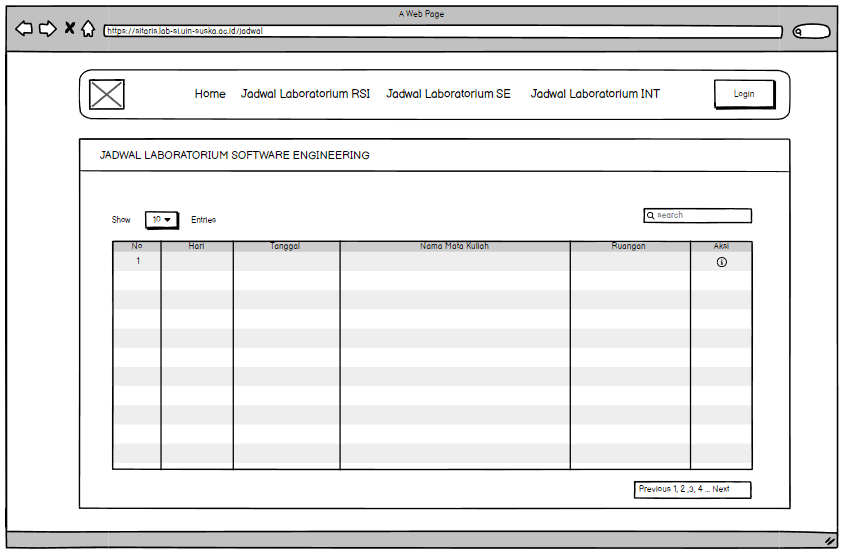
\includegraphics[width=0.82\textwidth]{konten/gambar/user interface/ui-jadwal-se.png}
		      \caption{Tampilan Kelola Jadwal Laboratorium}
		      \label{fig:jadwal}
	      \end{figure}
	      \begin{figure}
		      \centering
		      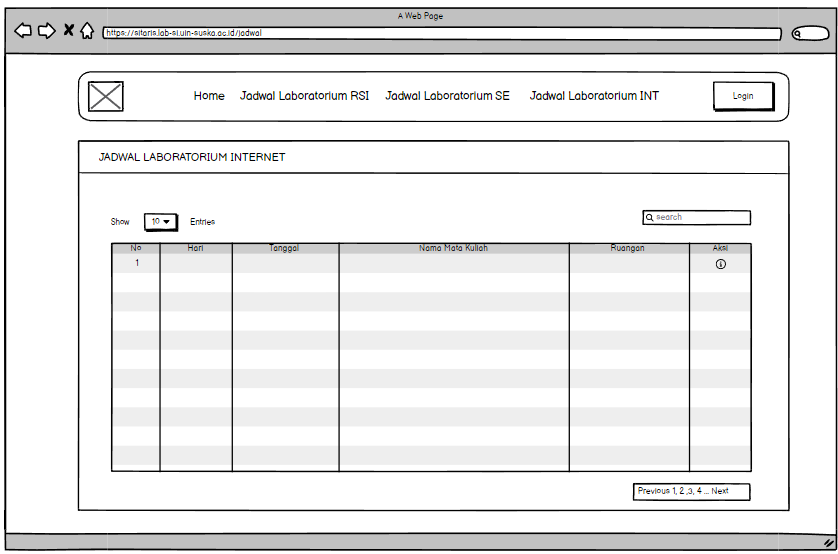
\includegraphics[width=0.82\textwidth]{konten/gambar/user interface/ui-jadwal-int.png}
		      \caption{Tampilan Kelola Jadwal Laboratorium}
		      \label{fig:jadwal}
	      \end{figure}
	\item Rancangan tampilan tambah jadwal yang berfungsi untuk menambah jadwal laboratorium dapat dilihat pada \pic~\ref{fig:jadwal}
	      \begin{figure}
		      \centering
		      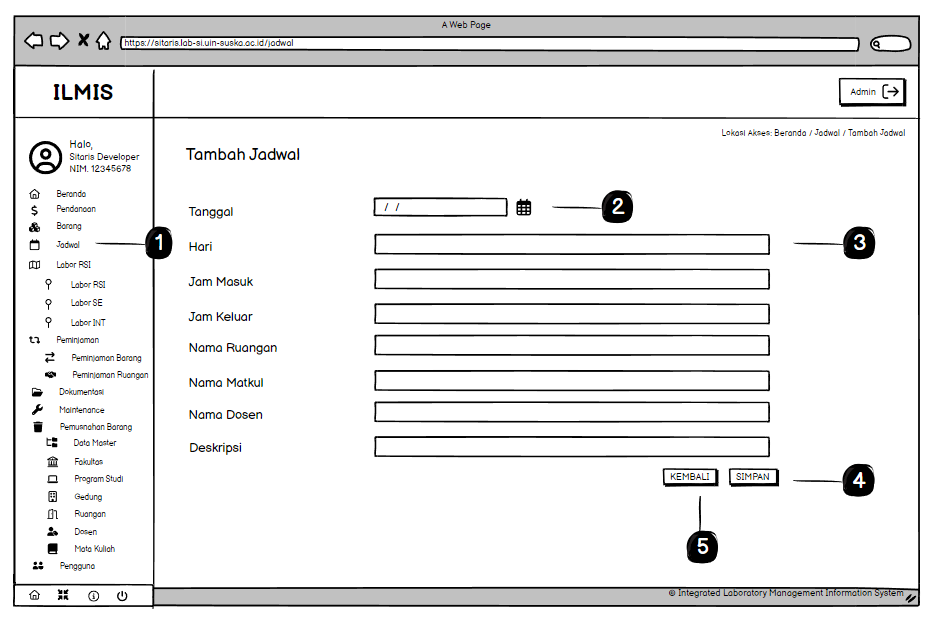
\includegraphics[width=0.82\textwidth]{konten/gambar/tambah-jadwal.png}
		      \caption{Tampilan Tambah Jadwal Laboratorium}
		      \label{fig:jadwal}
	      \end{figure}
	      \begin{table}[H]
		      \centering
		      \caption{Tabel Keterangan Tampilan Tambah Jadwal}
		      \begin{tabular}{|c|p{0.55\textwidth}|}
			      \hline
			      \textbf{Nomor Callouts} & \textbf{Keterangan}                                                                                                                                           \\
			      \hline
			      1                       & Berisi menu navigasi dengan ikon dan teks, menggunakan font-family: Poppins, font-size: 14px. Memiliki warna latar gelap dan ikon menu terorganisir vertikal. \\
			      2                       & Field input untuk memasukkan tanggal dengan placeholder dd/mm/yyyy. Terdapat ikon kalender di sebelah kanan untuk membantu memilih tanggal.                   \\
			      3                       & Berisi beberapa form input untuk memasukkan data berikut:                                                                                                     \\
			                              & - Hari: Input teks untuk memilih atau memasukkan hari.                                                                                                        \\
			                              & - Jam Masuk dan Jam Keluar: Input waktu dengan ikon jam di sebelah kanan.                                                                                     \\
			                              & - Nama Ruangan, Nama Mata Kuliah, dan Nama Dosen: Dropdown untuk memilih opsi.                                                                                \\
			                              & - Deskripsi: Area teks kosong untuk menambahkan keterangan lebih lanjut.                                                                                      \\
			      4                       & Dua tombol aksi:                                                                                                                                              \\
			                              & - Tombol Kembali: Berwarna merah (\#FF5A5F) dengan padding: 12px 24px, border-radius: 6px.                                                                    \\
			                              & - Tombol Simpan: Berwarna biru (\#2563EB) dengan padding: 12px 24px, border-radius: 6px.                                                                      \\
			      5                       & Teks di bagian bawah layar yang menampilkan informasi seperti hak cipta atau detail versi aplikasi. Font-size kecil dengan warna abu-abu muda.                \\
			      \hline
		      \end{tabular}
	      \end{table}

	\item Rancangan tampilan edit jadwal yang berfungsi untuk mengedit jadwal laboratorium dapat dilihat pada \pic~\ref{fig:edit-jadwal}
	      \begin{figure}
		      \centering
		      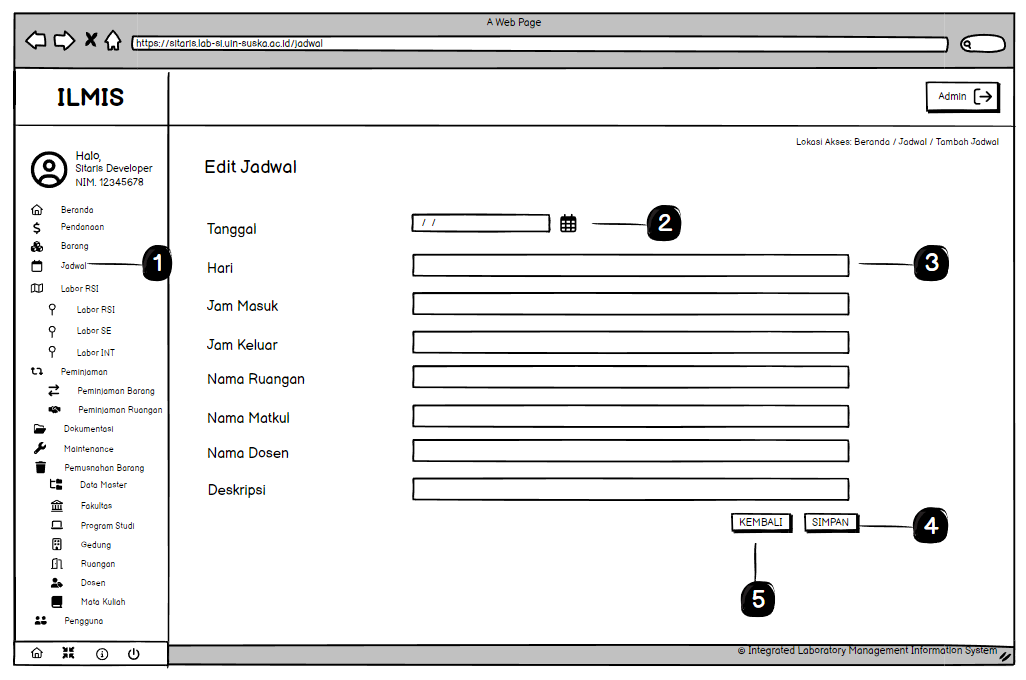
\includegraphics[width=0.82\textwidth]{konten/gambar/user interface/edit-jadwal.png}
		      \caption{Tampilan Edit Jadwal Laboratorium}
		      \label{fig:edit-jadwal}
	      \end{figure}
	\item Rancangan tampilan kelola mata kuliah yang berfungsi untuk mengelola mata kuliah laboratorium dapat dilihat pada \pic~\ref{fig:matkul}
	      \begin{figure}
		      \centering
		      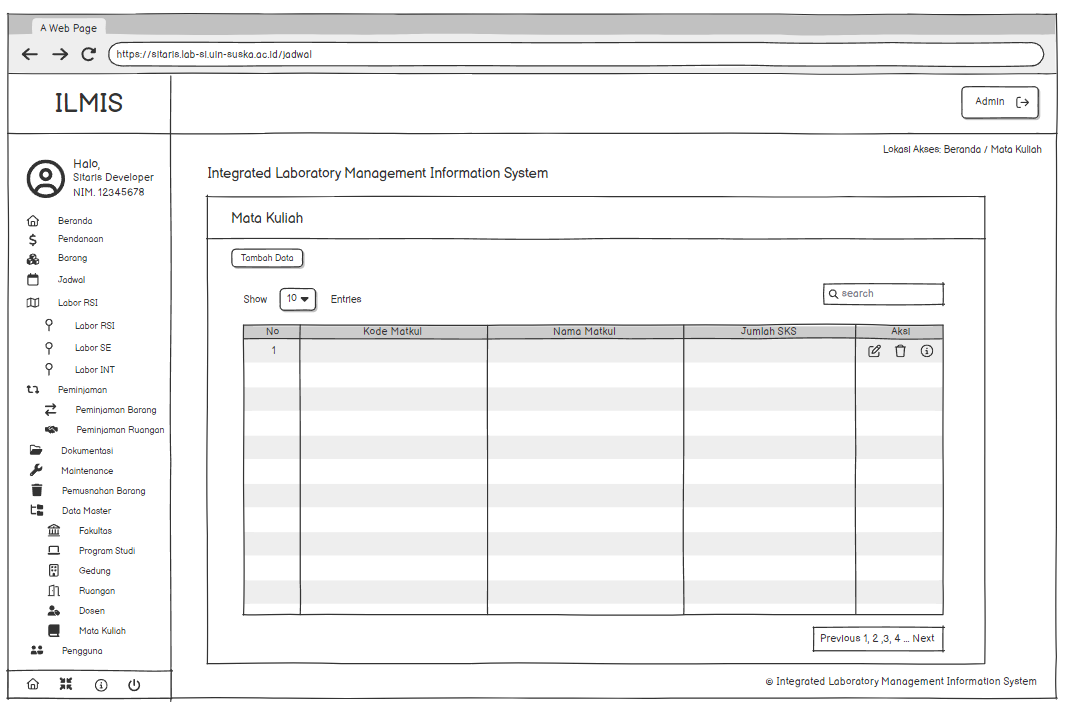
\includegraphics[width=0.82\textwidth]{konten/gambar/user interface/ui-matkul.png}
		      \caption{Tampilan Kelola Mata Kuliah Laboratorium}
		      \label{fig:matkul}
	      \end{figure}
	\item Rancangan tampilan tambah mata kuliah yang berfungsi untuk menambah mata kuliah dapat dilihat pada \pic~\ref{fig:tambah-matkul}
	      \begin{figure}
		      \centering
		      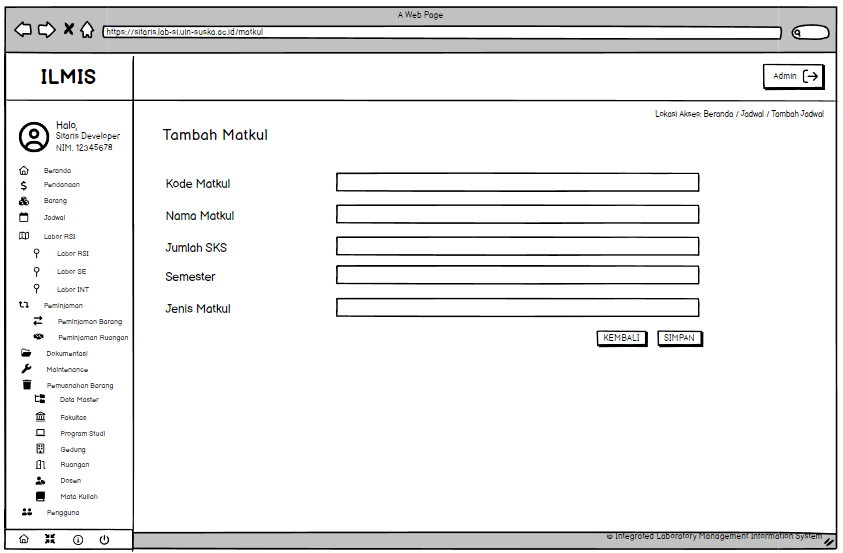
\includegraphics[width=0.82\textwidth]{konten/gambar/user interface/tambah-matkul.png}
		      \caption{Tampilan Tambah Mata Kuliah Laboratorium}
		      \label{fig:tambah-matkul}
	      \end{figure}
	\item Rancangan tampilan edit mata kuliah yang berfungsi untuk mengedit mata kuliah laboratorium dapat dilihat pada \pic~\ref{fig:edit-matkul}
	      \begin{figure}
		      \centering
		      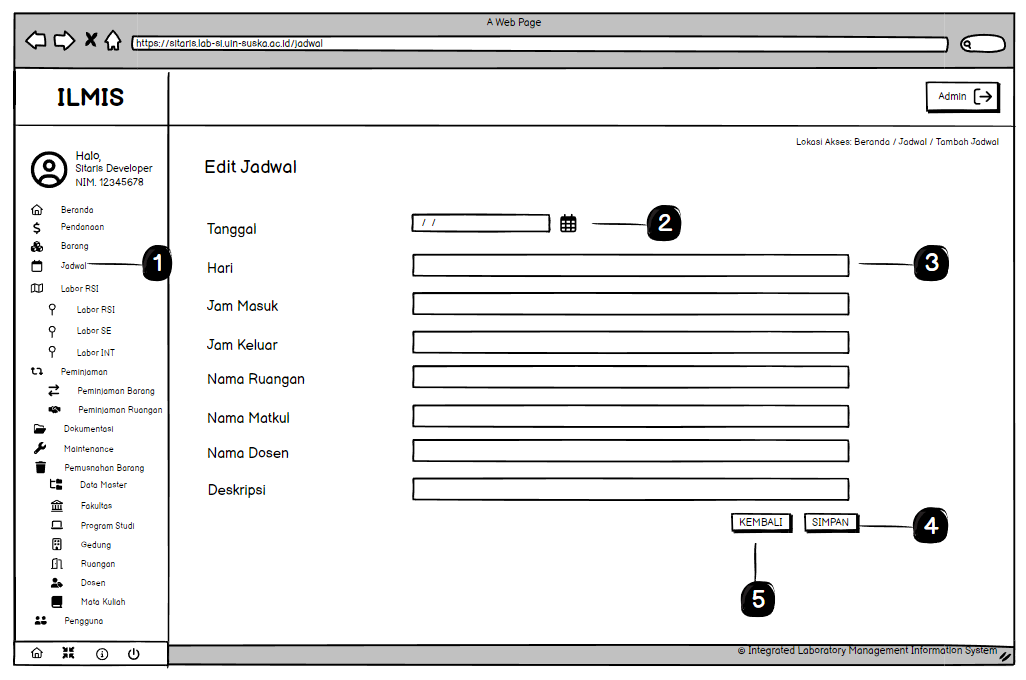
\includegraphics[width=0.82\textwidth]{konten/gambar/user interface/edit-jadwal.png}
		      \caption{Tampilan Edit Mata Kuliah Laboratorium}
		      \label{fig:edit-matkul}
	      \end{figure}
	\item Rancangan tampilan kelola dosen yang berfungsi untuk mengelola dosen laboratorium dapat dilihat pada \pic~\ref{fig:dosen}
	      \begin{figure}
		      \centering
		      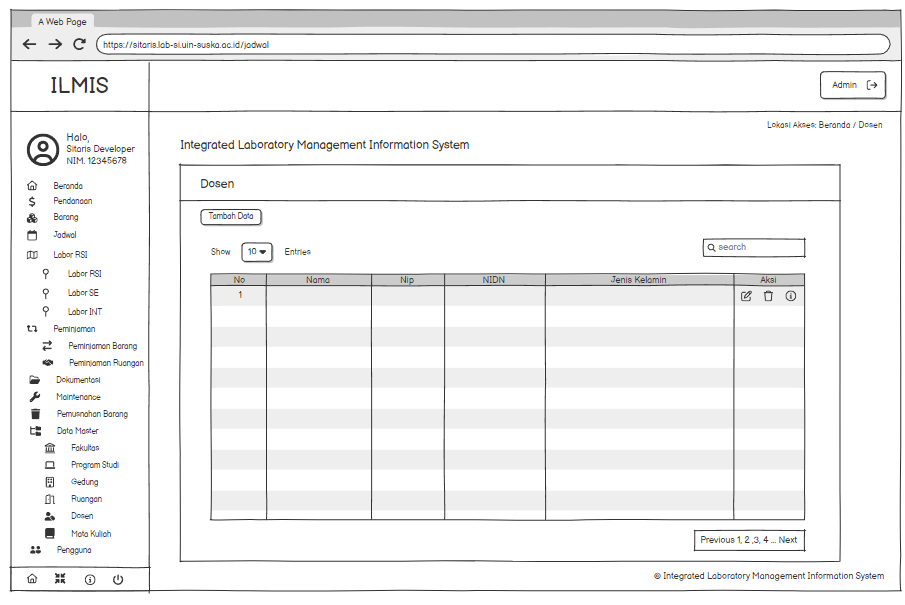
\includegraphics[width=0.82\textwidth]{konten/gambar/user interface/ui-dosen.png}
		      \caption{Tampilan Kelola Dosen Laboratorium}
		      \label{fig:dosen}
	      \end{figure}
	\item Rancangan tampilan tambah dosen yang berfungsi untuk menambah dosen laboratorium dapat dilihat pada \pic~\ref{fig:tambah-dosen}
	      \begin{figure}
		      \centering
		      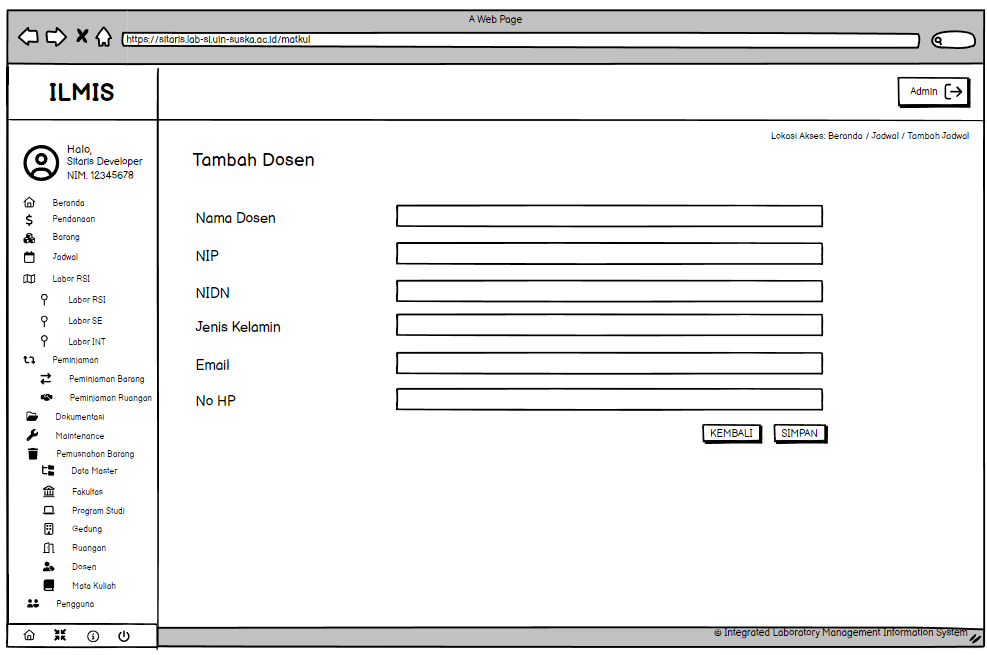
\includegraphics[width=0.82\textwidth]{konten/gambar/user interface/tambah-dosen.png}
		      \caption{Tampilan Tambah Dosen Laboratorium}
		      \label{fig:tambah-dosen}
	      \end{figure}
	\item Rancangan tampilan edit dosen yang berfungsi untuk mengelola dosen laboratorium dapat dilihat pada \pic~\ref{fig:edit-dosen}
	      \begin{figure}
		      \centering
		      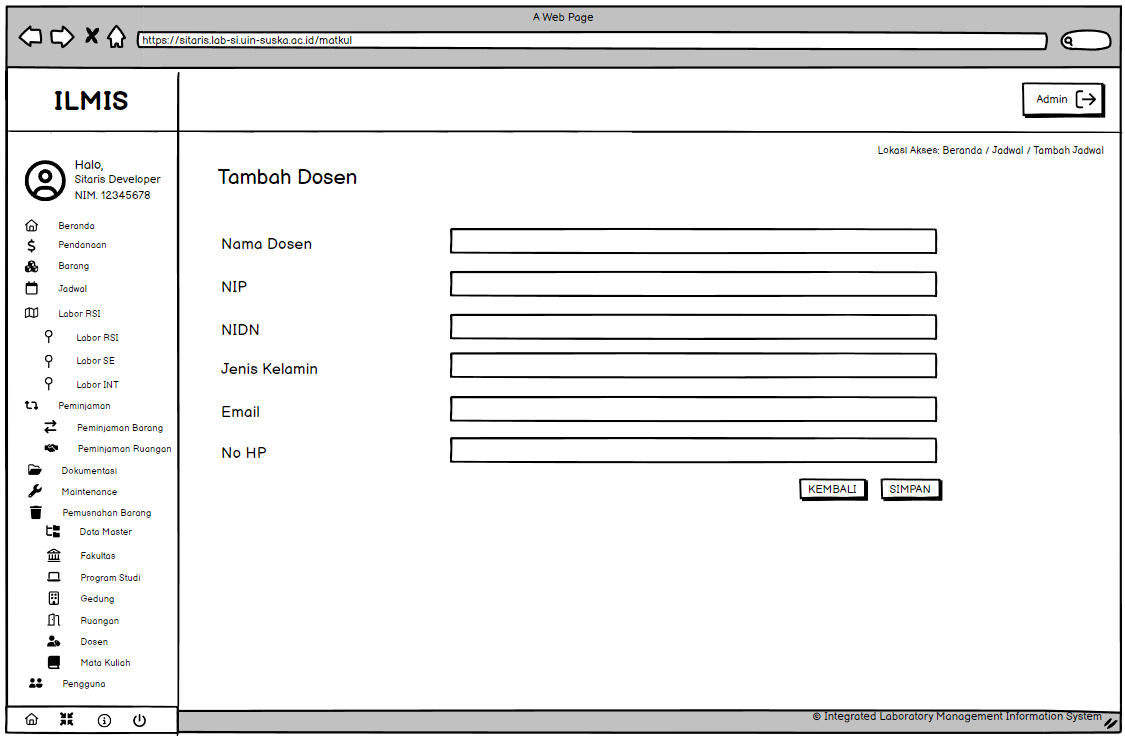
\includegraphics[width=0.82\textwidth]{konten/gambar/user interface/edit-dosen.png}
		      \caption{Tampilan Edit Dosen Laboratorium}
		      \label{fig:edit-dosen}
	      \end{figure}
\end{enumerate}


\ifthenelse{\equal{\tipeta}{TUGAS AKHIR}}{
	%-----------------------------------------------------------------------------------------------%
%
% Maret 2019
% Template Latex untuk Tugas Akhir Program Studi Sistem informasi ini
% dikembangkan oleh Inggih Permana (inggihjava@gmail.com)
%
% Template ini dikembangkan dari template yang dibuat oleh Andreas Febrian (Fasilkom UI 2003).
%
% Orang yang cerdas adalah orang yang paling banyak mengingat kematian.
%
%-----------------------------------------------------------------------------------------------%

%-----------------------------------------------------------------------------%
\chapter{\babLima}

\section{Implementasi Sistem}
Implementasi sistem merupakan tahap dimana sistem yang telah dirancang akan dijalankan. Implementasi sistem ini meliputi implementasi \textit{database}, implementasi \textit{routes}, implementasi \textit{model}, implementasi \textit{view}, dan implementasi \textit{controller}. Implementasi sistem ini dilakukan dengan menggabungkan 2 \textit{framework} yaitu Laravel dan Codeigniter.

\section{Batasan Implementasi}
Batasan implementasi Sistem Informasi Inventaris Laboratorium (SITARIS) dalam penelitian untuk Kerja Praktek ini adalah:
\begin{enumerate}
	\item Sistem yang dibangun memiliki \textit{platform} berbasis\textit{ Web}.
	\item Sistem yang dibangun memiliki hak akses seperti Admin, Kalab, Kaprodi, Sekprodi, dan Aslab.
	\item Menggunakan bahasa pemrograman PHP dengan \textit{framework} CodeIgniter dan \textit{database} MariaDB/PHPMyadmin.
	\item Sistem dapat menampilkan data barang, pendanaan, dokumentasi, peminjaman barang, peminjaman ruangan, \textit{maintenance}, pemusnahan barang, fakultas/lembaga, program studi/unit, gedung, ruangan, jadwal, dosen, mata kuliah dan pengguna.
\end{enumerate}

\section{Implementasi Perangkat Keras (\textit{Hardware})}
% -----------------------------------------------------------------------------%
Implementasi pada lingkungan \textit{hardware} adalah implementasi pada perangkat keras yang digunakan untuk menjalankan sistem informasi manajemen laboratorium. Implementasi \textit{hardware} yang digunakan dapat dilihat pada Tabel 5.1.

Minimum kebutuhan pada implementasi \textit{hardware} untuk menjalankan sistem informasi manajemen laboratorium adalah spesifikasi perangkat keras yang harus terpenuhi agar sistem dapat beroperasi secara optimal. Tabel 5.1. menyajikan daftar rinci dari komponen perangkat keras yang diperlukan dan spesifikasinya, yang mencakup prosesor, RAM, Hardisk, Monitor, dan perangkat masukan yang harus memenuhi standar minimum agar sistem berfungsi dengan baik.

\begin{longtable}{l l}
	\caption{Spesifikasi Perangkat Keras (\textit{Hardware})} \\
	\hline
	\textbf{Komponen \textit{Hardware}} & \textbf{Spesifikasi} \\ 
	\hline
	\endfirsthead
	
	\multicolumn{2}{c}{\tablename\ \thetable\ {Spesifikasi Perangkat Keras (\textit{Hardware})} \space (Tabel lanjutan...)} \\
	\hline
	\textbf{Komponen \textit{Hardware}} & \textbf{Spesifikasi} \\ 
	\hline
	\endhead
	
	Processor                           & Intel \textregistered{} CoreTM i3-4160, 3.60GHz \\
	Memory (RAM)                        & 2 GB                                            \\
	Hardisk (HDD)                       & 1 TB                                            \\
	LCD                                 & Lenovo 17"                                      \\
	\hline
\end{longtable}

\section{Implementasi Perangkat Lunak (\textit{Software})}
% -----------------------------------------------------------------------------%
Implementasi pada lingkungan \textit{software} adalah implementasi pada perangkat lunak yang digunakan untuk menjalankan sistem informasi inventaris laboratorium. Implementasi \textit{software} yang digunakan dapat dilihat pada Tabel 5.2.

\begin{longtable}{l l}
	\caption{Spesifikasi Perangkat Lunak (\textit{Software})} \\
	\hline
	\textbf{Komponen \textit{Software}} & \textbf{Spesifikasi} \\ 
	\hline
	\endfirsthead
	
	\multicolumn{2}{c}{\tablename\ \thetable\ {Spesifikasi Perangkat Lunak (\textit{Software})} \space (Tabel lanjutan...)} \\
	\hline
	\textbf{Komponen \textit{Software}} & \textbf{Spesifikasi} \\ 
	\hline
	\endhead
	
	Sistem Operasi                      & Windows 7, 8, 10, dan 11          \\
	Browser                             & Google Chrome dan Mozilla Firefox \\
	Bahasa Pemrograman                  & PHP dan Javascript                \\
	Web \textit{Database}               & MariaDB                           \\
	\textit{Framework}                  & CodeIgniter 4                     \\
	\hline
\end{longtable}

\subsection{Implementasi \textit{Database}}
Pada implementasi \textit{database} ini nama yang digunakan adalah ”man\_lab”. Implemenasi \textit{database} ini terdapat beberapa tabel yang akan digunakan dalam sistem. Pembuatan \textit{database} dilakukan dengan menggunakan \textit{database} MariaDB. Tabel-tabel ini akan digunakan untuk menyimpan data-data yang diperlukan dalam sistem. Berikut adalah struktur tabel yang telah diintegrasikan dan digunakan dalam sistem ini dapat dilihat pada Gambar \ref{database-manlab}.

\begin{figure}
	\centering
	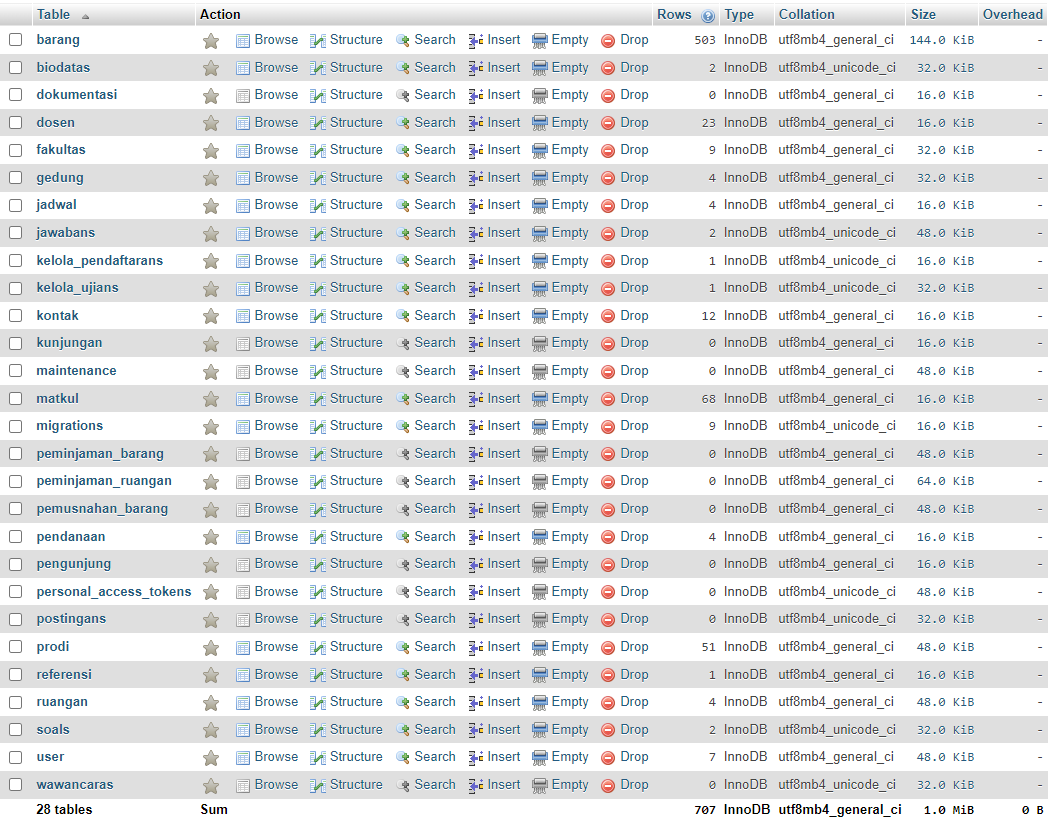
\includegraphics[width=1\textwidth]{konten/gambar/implementasi/database.png}
	\caption{\textit{Database}}
	\label{database-manlab}
\end{figure}

Pada pengembangan kali ini dilakukan penambahan tabel baru yaitu tabel "jadwal", "dosen", "mata kuliah", dan tabel  "biodatas", "users", "kelola pendaftarans", "kelola ujians", "postingans", "soals", jawabans", dan "wawancaras" sebagai tabel tambahan untuk integrasi sistem.

\begin{enumerate}

	\item Tabel Dosen dirancang untuk menyimpan informasi penting terkait dosen dalam sebuah sistem informasi. Kolom id\_dosen berfungsi sebagai kunci utama (primary key) yang memastikan setiap data dosen bersifat unik dan tidak terjadi duplikasi. Kolom nama\_dosen digunakan untuk mencatat nama lengkap dosen, sedangkan nip\_dosen menyimpan Nomor Induk Pegawai (NIP) sebagai identitas resmi dosen, jika tersedia. Untuk mencatat jenis kelamin, digunakan kolom jenis\_kelamin dengan opsi seperti "Laki-laki" atau "Perempuan". Informasi kontak dosen dicatat melalui kolom email\_dosen dan no\_hp, yang masing-masing menyimpan alamat email serta nomor handphone. Selain itu, kolom nidn digunakan untuk menyimpan Nomor Induk Dosen Nasional (NIDN) sebagai identitas unik dosen di tingkat nasional. Semua kolom ini dirancang untuk memastikan data dosen tersimpan secara lengkap, terstruktur, dan mudah diakses. Tampilan dapat dilihat pada Gambar \ref{tabel-Dosen}.

	      \begin{figure}
		      \centering
		      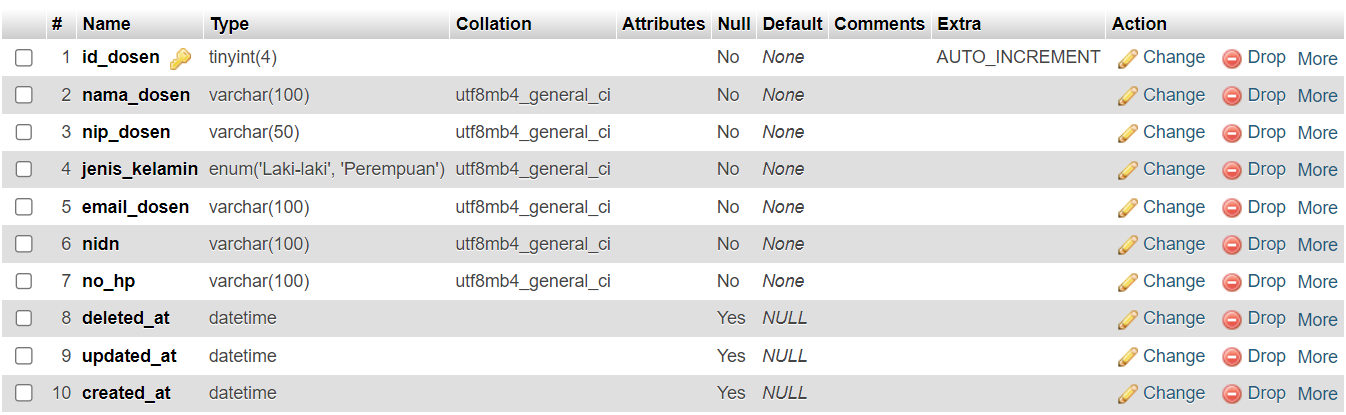
\includegraphics[width=0.82\textwidth]{konten/gambar/implementasi/tabel-dosen.png}
		      \caption{Tampilan \textit{Database} Tabel Dosen}
		      \label{tabel-Dosen}
	      \end{figure}


	\item Tabel Matkul digunakan untuk menyimpan informasi mengenai mata kuliah dalam sistem informasi akademik. Kolom id\_matkul berfungsi sebagai kunci utama (primary key) untuk mengidentifikasi setiap mata kuliah secara unik dan mencegah terjadinya duplikasi data. Kolom kode\_matkul menyimpan kode unik mata kuliah sebagai referensi singkat. Nama mata kuliah dicatat dalam kolom nama\_matkul untuk memberikan informasi deskriptif terkait mata kuliah tersebut. Kolom sks digunakan untuk mencatat jumlah Sistem Kredit Semester (SKS) dari mata kuliah, sedangkan semester mencatat pada semester berapa mata kuliah tersebut ditawarkan. Selain itu, kolom jenis\_matkul digunakan untuk mengklasifikasikan jenis mata kuliah, misalnya wajib dan pilihan. Struktur tabel ini dirancang untuk memastikan data terkait mata kuliah tersimpan secara terorganisasi dan mudah diakses sesuai kebutuhan. Tampilan dapat dilihat pada Gambar \ref{tabel-Matkul}.

	      \begin{figure}
		      \centering
		      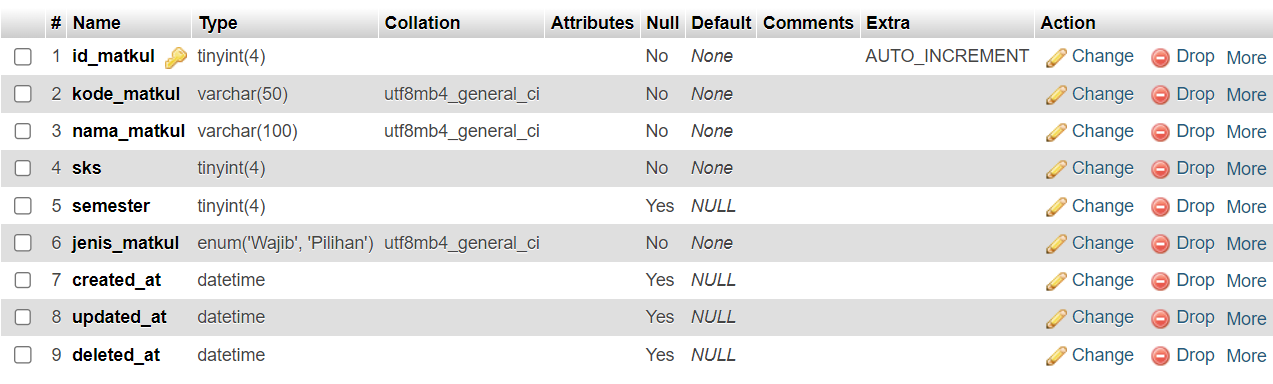
\includegraphics[width=0.82\textwidth]{konten/gambar/implementasi/tabel-matkul.png}
		      \caption{Tampilan \textit{Database} Tabel Matkul}
		      \label{tabel-Matkul}
	      \end{figure}

	\item Tabel Jadwal  terdiri dari kolom id\_jadwal yang menjadi kunci utama dari tabel tersebut yang digunakan sebagai penanda agar tidak terjadi duplikasi data, id\_ruangan digunakan untuk menunjukkan ruangan yang digunakan, id\_matkul digunakan untuk menunjukkan mata kuliah yang digunakan, id\_dosen digunakan untuk menunjukkan dosen yang mengajar, tanggal digunakan untuk menunjukkan tanggal pelaksanaan, hari digunakan untuk menunjukkan hari laboratorium digunakan, jam\_masuk dan jam\_keluar digunakan untuk menunjukkan jam digunakannya laboratorium, dan deskripsi digunakan untuk menunjukkan deskripsi dari jadwal tersebut. Tampilan dapat dilihat pada Gambar \ref{tabel-jadwal}.

	      \begin{figure}
		      \centering
		      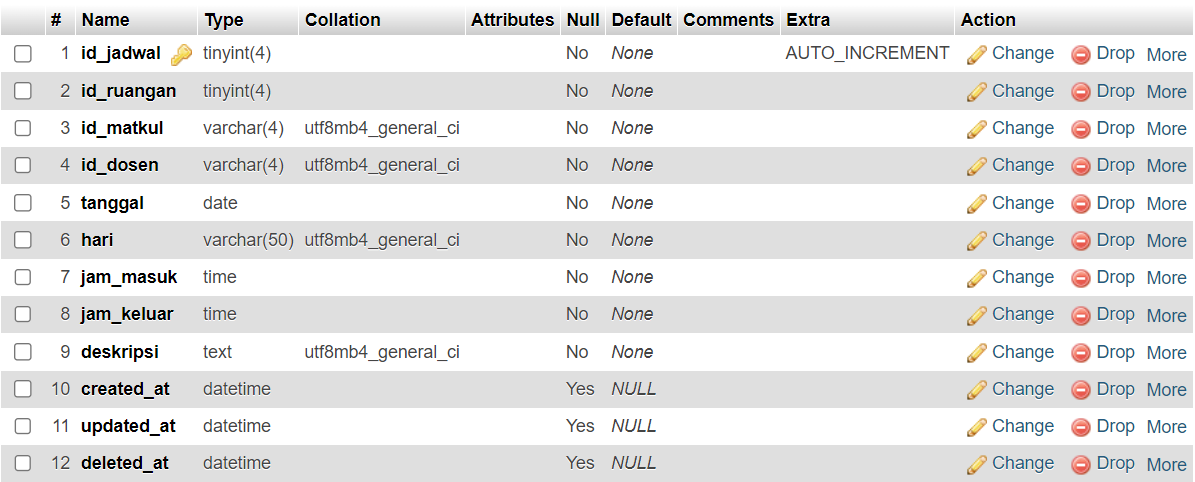
\includegraphics[width=0.82\textwidth]{konten/gambar/implementasi/tabel-jadwal.png}
		      \caption{Tampilan \textit{Database} Tabel Jadwal}
		      \label{tabel-jadwal}
	      \end{figure}

	\item Tabel Ruangan terdiri dari kolom id\_ruangan yang menjadi kunci utama dari tabel tersebut yang digunakan sebagai penanda agar tidak terjadi duplikasi data, id\_gedung menjadi kunci asing dalam tabel ruangan karena nama gedung diperlukan dalam pencatatan data ruangan, nama\_ruangan adalah kolom yang menyimpan nama ruangan yang dicatat, deskripsi\_ruangan menjelaskan detail tentang ruangan yang dicatat, gambar\_ruangan merupakan kolom untuk menyimpan data gambar dari ruangan yang dicatat. Tampilan dapat dilihat pada Gambar \ref{fig:tabel-ruangan}.

	      \begin{figure}
		      \centering
		      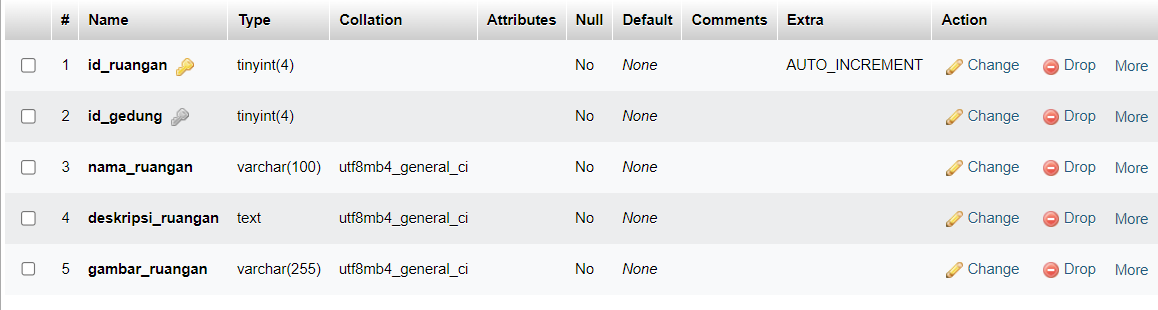
\includegraphics[width=0.82\linewidth]{konten//gambar/Tampilan database tabel ruangan.png}
		      \caption{Tampilan \textit{Database} Tabel Ruangan}
		      \label{fig:tabel-ruangan}
	      \end{figure}

	\item Tabel User terdiri dari kolom id\_user yang menjadi kunci utama dari tabel tersebut yang digunakan sebagai penanda agar tidak terjadi duplikasi data, nama merupakan kolom yang menyimpan nama pengguna, foto merupakan kolom untuk menyimpan foto profil pengguna, no\_identitas merupakan kolom yang digunakan untuk menyimpan data NIM, NIP, atau NIK dari pengguna, \textit{username} merupakan kolom yang digunakan untuk menyimpan \textit{username} pengguna, password\_hash merupakan kolom yang digunakan untuk menyimpan \textit{password} pengguna, email merupakan kolom yang digunakan untuk menyimpan email pengguna, role\_user merupakan kolom yang digunakan untuk menyimpan level akses pengguna. Tampilan dapat dilihat pada Gambar \ref{fig:tabel-user}.

	      \begin{figure}
		      \centering
		      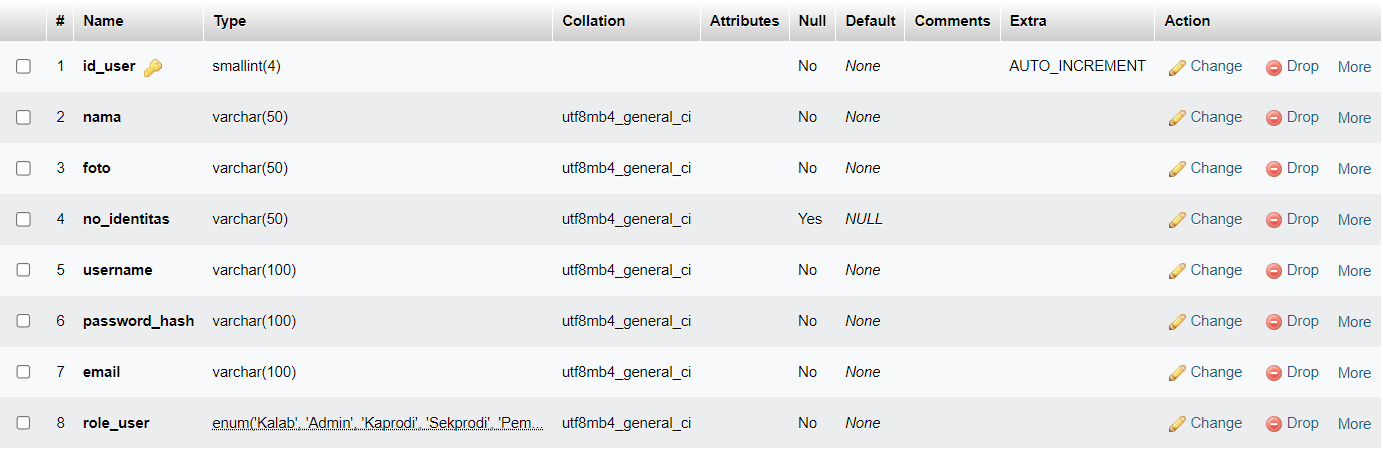
\includegraphics[width=0.82\linewidth]{konten//gambar/Tampilan database tabel user.png}
		      \caption{Tampilan \textit{Database} Tabel \textit{User}}
		      \label{fig:tabel-user}
	      \end{figure}
\end{enumerate}

\subsection{Implementasi \textit{Routes}}
\textit{Routes} dalam konsep MVC (\textit{Model-View-Controller}) adalah mekanisme yang digunakan untuk mengatur bagaimana permintaan \textit{(requests)} dari pengguna atau klien akan ditangani oleh aplikasi web. Routes menentukan hubungan antara URL yang diminta oleh pengguna dengan controller yang akan menangani permintaan tersebut \cite{kelvin2022sistem}. Dalam pengembangan ini ditambahkan beberapa \textit{routes} untuk menangani \textit{requests} pada sistem informasi.

\begin{enumerate}
	\item \textit{Routes} dalam implementasi Sistem Manajemen Laboratorium pada data dosen dapat dilihat pada Gambar \ref{fig:routes-dosen}
	      \begin{figure}
		      \centering
		      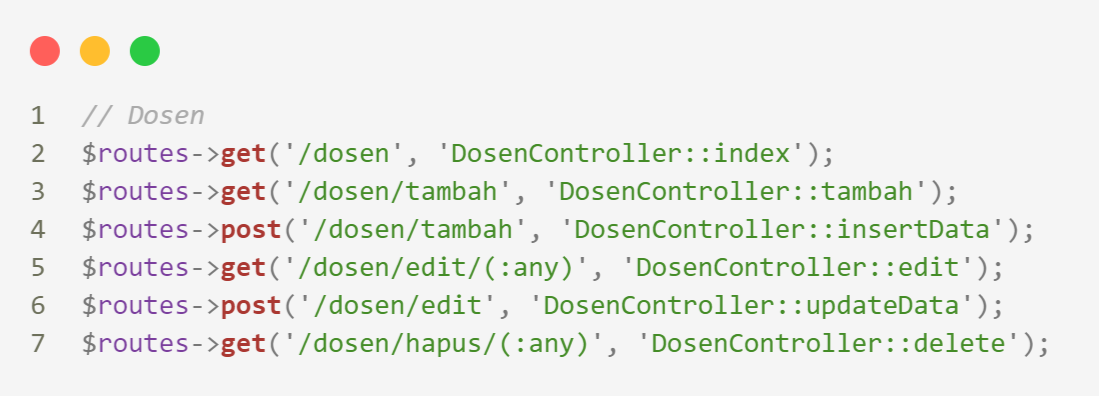
\includegraphics[width=0.82\linewidth]{konten//gambar/routes/dosen.png}
		      \caption{Tampilan \textit{Routes} Dosen}
		      \label{fig:routes-dosen}
	      \end{figure}
	\item \textit{Routes} dalam implementasi Sistem Manajemen Laboratorium pada data matkul dapat dilihat pada Gambar \ref{fig:routes-matkul}
	      \begin{figure}
		      \centering
		      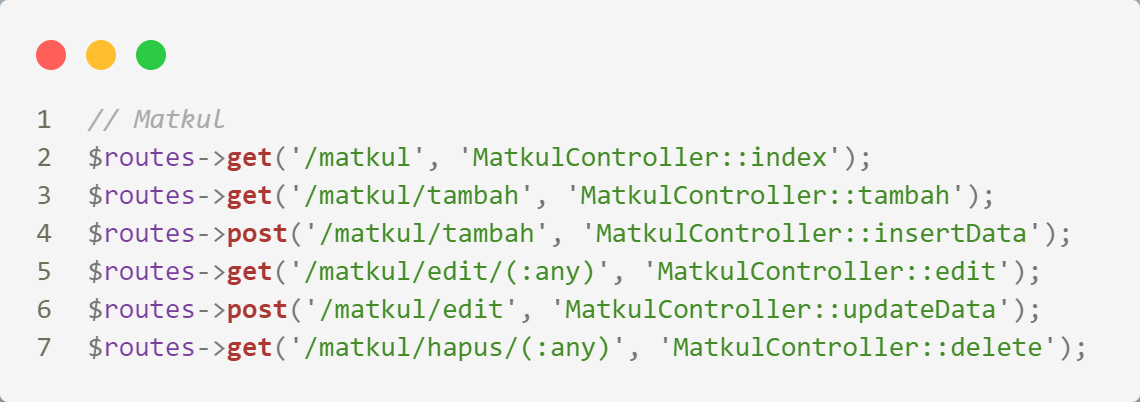
\includegraphics[width=0.82\linewidth]{konten//gambar/routes/matkul.png}
		      \caption{Tampilan \textit{Routes} Matkul}
		      \label{fig:routes-matkul}
	      \end{figure}
	\item \textit{Routes} dalam implementasi Sistem Manajemen Laboratorium pada data jadwal dapat dilihat pada Gambar \ref{fig:routes-jadwal}
	      \begin{figure}
		      \centering
		      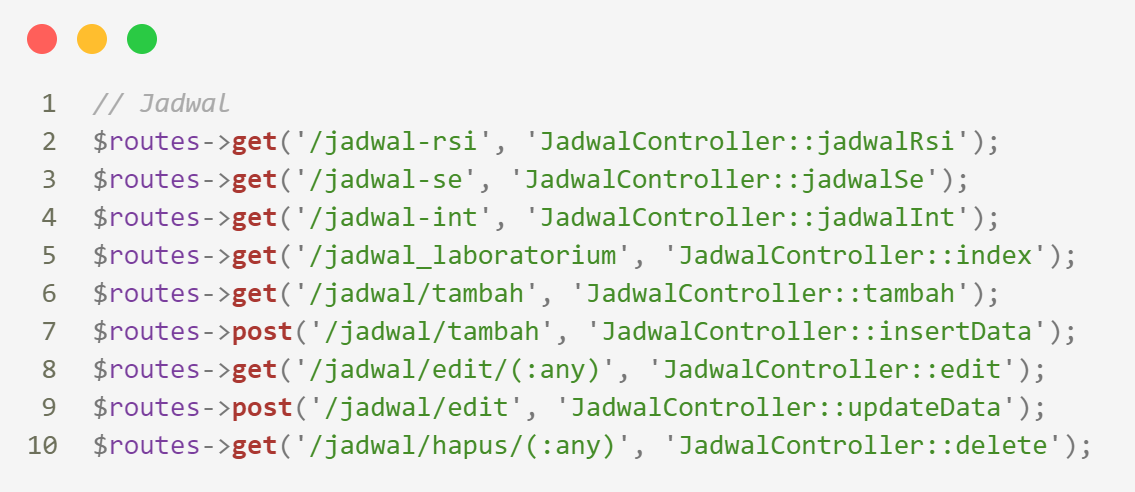
\includegraphics[width=0.82\linewidth]{konten//gambar/routes/jadwal.png}
		      \caption{Tampilan \textit{Routes} Jadwal}
		      \label{fig:routes-jadwal}
	      \end{figure}
	\item \textit{Routes} dalam implementasi Sistem Manajemen Laboratorium pada data ruangan dapat dilihat pada Gambar \ref{fig:routes-ruangan}
	      \begin{figure}
		      \centering
		      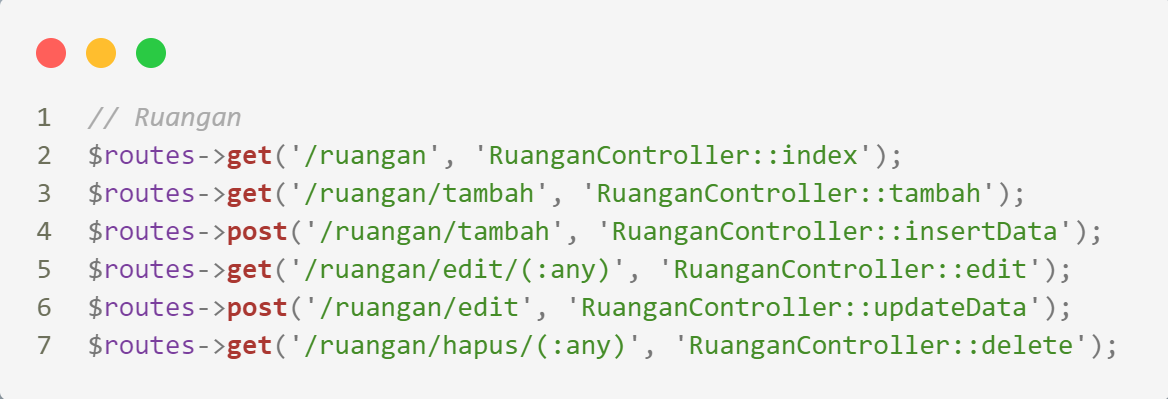
\includegraphics[width=0.82\linewidth]{konten//gambar/routes/ruangan.png}
		      \caption{Tampilan \textit{Routes} Ruangan}
		      \label{fig:routes-ruangan}
	      \end{figure}
	\item \textit{Routes} dalam implementasi Sistem Manajemen Laboratorium pada data user dapat dilihat pada Gambar \ref{fig:routes-user}
	      \begin{figure}
		      \centering
		      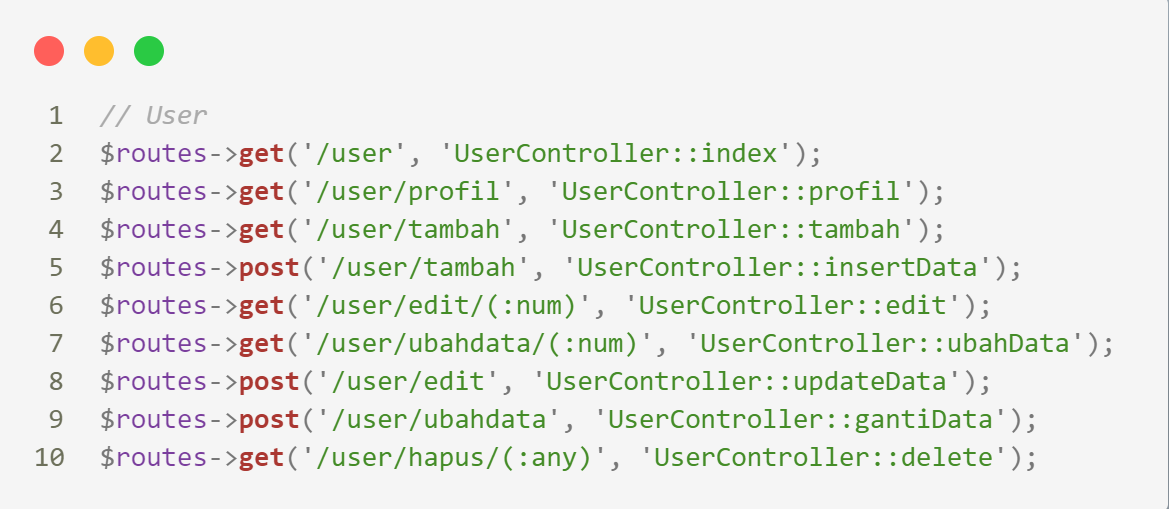
\includegraphics[width=0.82\linewidth]{konten//gambar/routes/user.png}
		      \caption{Tampilan \textit{Routes} \textit{User}}
		      \label{fig:routes-user}
	      \end{figure}
\end{enumerate}

\subsection{Implementasi \textit{Model}}
Model adalah komponen yang bertanggung jawab untuk mengatur data, aturan bisnis, dan logika aplikasi. Ini merupakan representasi dari data dalam aplikasi. Model mengelola semua operasi data, seperti pengambilan, pembaruan, dan penyimpanan data \cite{firdaus2020rancang}. Model-model ini akan diatur pada folder app/model pada \textit{framework} CodeIgniter dapat dilihat pada gambar \ref{fig:implementasi-model}

\begin{figure}
	\centering
	\includegraphics[width=0.82\linewidth]{konten//gambar/implementasi-folder/folder-model.png}
	\caption{Implementasi Model}
	\label{fig:implementasi-model}
\end{figure}

% \begin{enumerate}
% 	\item \textit{Model} dalam implementasi Sistem Manajemen Laboratorium pada data dosen dapat dilihat pada Gambar \ref{fig:model-dosen}
% 	      \begin{figure}
% 		      \centering
% 		      \includegraphics[width=0.82\linewidth]{konten//gambar/model/dosen.png}
% 		      \caption{Tampilan Model Dosen}
% 		      \label{fig:model-dosen}
% 	      \end{figure}
% 	\item \textit{Routes} dalam implementasi Sistem Manajemen Laboratorium pada data matkul dapat dilihat pada Gambar \ref{fig:model-matkul}
% 	      \begin{figure}
% 		      \centering
% 		      \includegraphics[width=0.82\linewidth]{konten//gambar/model/matkul.png}
% 		      \caption{Tampilan Model Matkul}
% 		      \label{fig:model-matkul}
% 	      \end{figure}
% 	\item \textit{Routes} dalam implementasi Sistem Manajemen Laboratorium pada data jadwal dapat dilihat pada Gambar \ref{fig:model-jadwal}
% 	      \begin{figure}
% 		      \centering
% 		      \includegraphics[width=0.82\linewidth]{konten//gambar/model/jadwal.png}
% 		      \caption{Tampilan Model Jadwal}
% 		      \label{fig:model-jadwal}
% 	      \end{figure}
% 	\item \textit{Routes} dalam implementasi Sistem Manajemen Laboratorium pada data ruangan dapat dilihat pada Gambar \ref{fig:model-ruangan}
% 	      \begin{figure}
% 		      \centering
% 		      \includegraphics[width=0.82\linewidth]{konten//gambar/model/ruangan.png}
% 		      \caption{Tampilan Model Ruangan}
% 		      \label{fig:model-ruangan}
% 	      \end{figure}
% 	\item \textit{Routes} dalam implementasi Sistem Manajemen Laboratorium pada data user dapat dilihat pada Gambar \ref{fig:model-user}
% 	      \begin{figure}
% 		      \centering
% 		      \includegraphics[width=0.82\linewidth]{konten//gambar/model/user.png}
% 		      \caption{Tampilan Model \textit{User}}
% 		      \label{fig:model-user}
% 	      \end{figure}
% \end{enumerate}

\subsection{Implementasi \textit{View}}
\textit{View }adalah komponen yang menampilkan antarmuka pengguna dan menampilkan data dari Model. \textit{View} mengamati perubahan pada Model dan \textit{Controller}, dan diperbarui sesuai keadaan terkini. Penggunaan \textit{View} memisahkan tugas penyajian dan manajemen data dalam aplikasi, yang memberikan fleksibilitas dan pemeliharaan yang lebih baik \cite{firdaus2020rancang}. \textit{View} ini akan diatur pada folder app/view pada \textit{framework} CodeIgniter dapat dilihat pada gambar \ref{fig:implementasi-view}

\begin{figure}
	\centering
	\includegraphics[width=0.82\linewidth]{konten//gambar/implementasi-folder/folder-view.png}
	\caption{Implementasi View}
	\label{fig:implementasi-view}
\end{figure}

\subsection{Implementasi \textit{Controller}}
\textit{Controller} adalah komponen yang bertanggung jawab untuk mengatur logika pengendalian atau interaksi antara Model (data), \textit{View} (tampilan), dan pengguna \cite{rahman2018perancangan}. \textit{Controller} ini akan diatur pada folder app/controller pada \textit{framework} CodeIgniter dapat dilihat pada gambar \ref{fig:implementasi-controller}

\begin{figure}
	\centering
	\includegraphics[width=0.82\linewidth]{konten//gambar/implementasi-folder/folder-controller.png}
	\caption{Implementasi Controller}
	\label{fig:implementasi-controller}
\end{figure}

\section{Hasil Implementasi}
Beberapa permasalahan yang teridentifikasi meliputi kesalahan dalam pembuatan kode barang (Lampiran B), disfungsi fitur peminjaman barang dan ruangan (Lampiran B), serta ketidaksesuaian format laporan akhir dengan kebutuhan kepala laboratorium (Lampiran B). Kesalahan dalam pembuatan kode barang menyebabkan ketidakakuratan dalam pencatatan dan pelacakan inventaris, yang dapat mengakibatkan kesulitan dalam manajemen barang. Disfungsi fitur peminjaman barang dan ruangan menghambat proses peminjaman yang seharusnya berjalan lancar, sehingga pengguna mengalami kesulitan dalam meminjam barang dan ruangan yang dibutuhkan. Ketidaksesuaian format laporan akhir dengan kebutuhan kepala laboratorium menyebabkan informasi yang disampaikan tidak sesuai dengan yang diharapkan, sehingga memerlukan penyesuaian agar laporan lebih relevan dan mudah dipahami. Saya sudah memperbaiki kesalahan ini dengan melakukan beberapa perubahan dan penyesuaian pada sistem. Hasil dari perbaikan tersebut akan saya tampilkan untuk menunjukkan peningkatan yang telah dicapai.

\begin{enumerate}
	\item Tampilan kode barang yang berfungsi untuk memberikan informasi mengenai kode barang dalam sistem manajemen laboratorium. Halaman ini memberikan gambaran umum tentang pengelolaan kode barang. Dapat dilihat pada Gambar \ref{fig:kode-barang}.
	      \begin{figure}
		      \centering
		      \includegraphics[width=0.82\textwidth]{konten/gambar/perbaikan/kode-barang.png}
		      \caption{Tampilan Kode Barang Sistem Manajemen Laboratorium}
		      \label{fig:kode-barang}
	      \end{figure}

	\item Tampilan pilihan peminjaman, yang memungkinkan pengguna memilih jenis peminjaman yang ingin dilakukan. Tampilan ini dirancang untuk memudahkan pengguna dalam menentukan pilihan peminjaman yang sesuai dengan kebutuhan mereka, dengan menyediakan opsi yang jelas dan terstruktur. Dapat dilihat pada Gambar \ref{fig:pilih-peminjaman}.
	      \begin{figure}
		      \centering
		      \includegraphics[width=0.82\textwidth]{konten/gambar/perbaikan/pilih-peminjaman.jpeg}
		      \caption{Tampilan Pilihan Peminjaman}
		      \label{fig:pilih-peminjaman}
	      \end{figure}
	\item Tampilan untuk pengelolaan peminjaman barang, yang memudahkan pengguna dalam mengatur dan melihat status peminjaman barang. Tampilan ini menyediakan fitur untuk menambah data peminjaman, serta menampilkan informasi peminjaman dalam format yang mudah dibaca. Dapat dilihat pada Gambar \ref{fig:peminjaman-barang}.
	      \begin{figure}
		      \centering
		      \includegraphics[width=0.82\textwidth]{konten/gambar/perbaikan/peminjaman-barang.jpeg}
		      \caption{Tampilan Pengelolaan Peminjaman Barang}
		      \label{fig:peminjaman-barang}
	      \end{figure}

	\item Tampilan untuk pengelolaan peminjaman ruangan, yang memungkinkan pengguna menambah data peminjaman ruangan ke dalam sistem. Tampilan ini dilengkapi dengan form input yang intuitif, sehingga pengguna dapat dengan mudah memasukkan detail peminjaman seperti waktu, tanggal, dan deskripsi kegiatan. Dapat dilihat pada Gambar \ref{fig:peminjaman-ruangan}.
	      \begin{figure}
		      \centering
		      \includegraphics[width=0.82\textwidth]{konten/gambar/perbaikan/peminjaman-ruangan.jpeg}
		      \caption{Tampilan Pengelolaan Peminjaman Ruangan}
		      \label{fig:peminjaman-ruangan}
	      \end{figure}

	\item Tampilan untuk memilih peminjam, yang memungkinkan pengguna menentukan peminjam yang akan melakukan peminjaman. Tampilan ini dilengkapi dengan daftar peminjam antara internal maupun eksternal, sehingga pengguna dapat dengan mudah memilih peminjam yang sesuai. Dapat dilihat pada Gambar \ref{fig:pilih-peminjam}.
	      \begin{figure}
		      \centering
		      \includegraphics[width=0.82\textwidth]{konten/gambar/perbaikan/pilih-peminjam.png}
		      \caption{Tampilan Pilih Peminjam}
		      \label{fig:pilih-peminjam}
	      \end{figure}
\end{enumerate}

Hasil implementasi \textit{interface} berfungsi untuk menunjukkan desain program sistem informasi manajemen laboratorium yang telah dilakukan penambahan. Hal ini dilakukan untuk mempermudah pengguna dalam memahami proses yang terdapat pada sistem informasi manajemen laboratorium tersebut.

\begin{enumerate}
	\item Tampilan \textit{landing page} yang berfungsi sebagai halaman pertama dari sistem informasi manajemen laboratorium. Halaman ini memberikan gambaran umum dan akses awal ke fitur-fitur sistem, serta menyambut pengguna dengan antarmuka yang ramah dan informatif. Dapat dilihat pada Gambar \ref{fig:landing-page}.
	      \begin{figure}
		      \centering
		      \includegraphics[width=0.82\textwidth]{konten/gambar/hasil/landing-page.jpeg}
		      \caption{Tampilan \textit{Landing Page} Sistem Manajemen Laboratorium}
		      \label{fig:landing-page}
	      \end{figure}
	\item Tampilan pilihan aplikasi untuk login, yang memungkinkan pengguna memilih aplikasi yang ingin diakses. Tampilan ini dirancang untuk memudahkan pengguna dalam menentukan aplikasi mana yang sesuai dengan kebutuhan mereka, dengan menyediakan opsi yang jelas dan terstruktur. Dapat dilihat pada Gambar \ref{fig:pilih-login}.
	      \begin{figure}
		      \centering
		      \includegraphics[width=0.82\textwidth]{konten/gambar/hasil/pilih-aplikasi.jpeg}
		      \caption{Tampilan Pilihan Aplikasi untuk Login}
		      \label{fig:pilih-login}
	      \end{figure}
	\item Tampilan untuk mengelola jadwal laboratorium, yang memudahkan pengguna dalam mengatur dan melihat jadwal kegiatan laboratorium. Tampilan ini menyediakan fitur untuk menambah, mengedit, dan menghapus jadwal, serta menampilkan jadwal dalam format yang mudah dibaca. Dapat dilihat pada \pic~\ref{fig:jadwal} sampai \pic~\ref{fig:jadwal-int}.
	      \begin{figure}
		      \centering
		      \includegraphics[width=0.82\textwidth]{konten/gambar/hasil/jadwal.jpeg}
		      \caption{Tampilan Pengelolaan Jadwal Laboratorium}
		      \label{fig:jadwal}
	      \end{figure}
	      \begin{figure}
		      \centering
		      \includegraphics[width=0.82\textwidth]{konten/gambar/hasil/labor-rsi.png}
		      \caption{Tampilan Pengelolaan Jadwal Laboratorium RSI}
		      \label{fig:jadwal-rsi}
	      \end{figure}
	      \begin{figure}
		      \centering
		      \includegraphics[width=0.82\textwidth]{konten/gambar/hasil/labor-se.png}
		      \caption{Tampilan Pengelolaan Jadwal Laboratorium SE}
		      \label{fig:jadwal-se}
	      \end{figure}
	      \begin{figure}
		      \centering
		      \includegraphics[width=0.82\textwidth]{konten/gambar/hasil/labor-int.png}
		      \caption{Tampilan Pengelolaan Jadwal Laboratorium INT}
		      \label{fig:jadwal-int}
	      \end{figure}
	\item Tampilan untuk menambah jadwal laboratorium, yang memungkinkan pengguna menambahkan jadwal baru ke dalam sistem. Tampilan ini dilengkapi dengan form input yang intuitif, sehingga pengguna dapat dengan mudah memasukkan detail jadwal seperti waktu, tanggal, dan deskripsi kegiatan. Dapat dilihat pada Gambar \ref{fig:tambah-jadwal}.
	      \begin{figure}
		      \centering
		      \includegraphics[width=0.82\textwidth]{konten/gambar/hasil/tambah-jadwal.jpeg}
		      \caption{Tampilan Tambah Jadwal Laboratorium}
		      \label{fig:tambah-jadwal}
	      \end{figure}
	\item Tampilan untuk mengedit jadwal laboratorium, yang memudahkan pengguna dalam melakukan perubahan pada jadwal yang sudah ada. Tampilan ini menyediakan fitur untuk memperbarui informasi jadwal dengan cepat dan efisien, serta memastikan bahwa semua perubahan tersimpan dengan baik. Dapat dilihat pada Gambar \ref{fig:edit-jadwal}.
	      \begin{figure}
		      \centering
		      \includegraphics[width=0.82\textwidth]{konten/gambar/hasil/edit-jadwal.jpeg}
		      \caption{Tampilan Edit Jadwal Laboratorium}
		      \label{fig:edit-jadwal}
	      \end{figure}
	\item Tampilan untuk mencetak jadwal laboratorium dalam format PDF, yang memudahkan pengguna untuk menyimpan dan membagikan jadwal dalam bentuk dokumen digital. Tampilan ini menyediakan fitur untuk mengonversi jadwal yang ada menjadi file PDF dengan cepat dan efisien. Dapat dilihat pada Gambar \ref{fig:cetak-jadwal}.
	      \begin{figure}
		      \centering
		      \includegraphics[width=0.82\textwidth]{konten/gambar/hasil/cetak-jadwal.png}
		      \caption{Tampilan Cetak Jadwal Laboratorium dalam Format PDF}
		      \label{fig:cetak-jadwal}
	      \end{figure}
	\item Tampilan untuk mengelola mata kuliah laboratorium, yang memungkinkan pengguna mengatur mata kuliah yang terkait dengan laboratorium. Tampilan ini menampilkan daftar mata kuliah yang dapat diakses dan dikelola, serta menyediakan opsi untuk menambah atau menghapus mata kuliah sesuai kebutuhan. Dapat dilihat pada Gambar \ref{fig:matkul}.
	      \begin{figure}
		      \centering
		      \includegraphics[width=0.82\textwidth]{konten/gambar/hasil/matkul.png}
		      \caption{Tampilan Kelola Mata Kuliah Laboratorium}
		      \label{fig:matkul}
	      \end{figure}
	\item Tampilan untuk menambah mata kuliah, yang memudahkan pengguna dalam menambahkan mata kuliah baru ke dalam sistem. Tampilan ini menyediakan form input yang lengkap untuk memasukkan informasi mata kuliah seperti nama, kode, dan deskripsi. Dapat dilihat pada Gambar \ref{fig:tambah-matkul}.
	      \begin{figure}
		      \centering
		      \includegraphics[width=0.82\textwidth]{konten/gambar/hasil/tambah-matkul.png}
		      \caption{Tampilan Tambah Mata Kuliah Laboratorium}
		      \label{fig:tambah-matkul}
	      \end{figure}
	\item Tampilan untuk mengedit mata kuliah laboratorium, yang memungkinkan pengguna melakukan perubahan pada mata kuliah yang sudah ada. Tampilan ini dirancang untuk memudahkan pengguna dalam memperbarui informasi mata kuliah dengan cepat dan akurat. Dapat dilihat pada Gambar \ref{fig:edit-matkul}.
	      \begin{figure}
		      \centering
		      \includegraphics[width=0.82\textwidth]{konten/gambar/hasil/edit-matkul.png}
		      \caption{Tampilan Edit Mata Kuliah Laboratorium}
		      \label{fig:edit-matkul}
	      \end{figure}
	\item Tampilan untuk mengedit mata kuliah laboratorium, yang memungkinkan pengguna melakukan perubahan pada mata kuliah yang sudah ada. Tampilan ini dirancang untuk memudahkan pengguna dalam memperbarui informasi mata kuliah dengan cepat dan akurat. Dapat dilihat pada Gambar \ref{fig:edit-matkul}.
	      \begin{figure}
		      \centering
		      \includegraphics[width=0.82\textwidth]{konten/gambar/hasil/edit-matkul.png}
		      \caption{Tampilan Edit Mata Kuliah Laboratorium}
		      \label{fig:edit-matkul}
	      \end{figure}
	\item Tampilan untuk mengelola dosen laboratorium, yang memudahkan pengguna dalam mengatur data dosen yang terkait dengan laboratorium. Tampilan ini menampilkan daftar dosen yang terdaftar dan menyediakan fitur untuk menambah, mengedit, atau menghapus data dosen. Dapat dilihat pada Gambar \ref{fig:dosen}.
	      \begin{figure}
		      \centering
		      \includegraphics[width=0.82\textwidth]{konten/gambar/hasil/dosen.png}
		      \caption{Tampilan Kelola Dosen Laboratorium}
		      \label{fig:dosen}
	      \end{figure}
	\item Tampilan untuk menambah dosen laboratorium, yang memungkinkan pengguna menambahkan data dosen baru ke dalam sistem. Tampilan ini dilengkapi dengan form input yang memudahkan pengguna dalam memasukkan informasi dosen seperti nama, NIDN, dan bidang keahlian. Dapat dilihat pada Gambar \ref{fig:tambah-dosen}.
	      \begin{figure}
		      \centering
		      \includegraphics[width=0.82\textwidth]{konten/gambar/hasil/tambah-dosen.png}
		      \caption{Tampilan Tambah Dosen Laboratorium}
		      \label{fig:tambah-dosen}
	      \end{figure}
	\item Tampilan untuk mengedit dosen laboratorium, yang memudahkan pengguna dalam melakukan perubahan pada data dosen yang sudah ada. Tampilan ini menyediakan fitur untuk memperbarui informasi dosen dengan mudah dan memastikan bahwa data yang tersimpan selalu akurat dan terkini. Dapat dilihat pada Gambar \ref{fig:edit-dosen}.
	      \begin{figure}
		      \centering
		      \includegraphics[width=0.82\textwidth]{konten/gambar/hasil/edit-dosen.png}
		      \caption{Tampilan Edit Dosen Laboratorium}
		      \label{fig:edit-dosen}
	      \end{figure}
\end{enumerate}

\section{Pengujian Sistem}
Metode Blackbox digunakan untuk menguji fitur-fitur yang ada pada sistem. Pengujian ini dilakukan untuk memastikan bahwa setiap fungsi dalam sistem berjalan sesuai dengan spesifikasi yang telah ditentukan. Metode ini hanya berfokus pada pengujian keluaran sistem berdasarkan masukan tertentu, tanpa memperhatikan proses internal atau struktur kode.

Pada pengujian Metode Blackbox, peneliti melakukan pengujian terhadap fitur-fitur yang ada pada sistem. Pengujian ini dilakukan oleh peneliti dan beberapa pengguna seperti Aslab dan Admin untuk memastikan bahwa fitur-fitur yang ada pada sistem berjalan dengan baik. Pengujian ini dapat dilihat pada Tabel~\ref{tab:PengujianBlackBox}

{
	\fontsize{10}{10}
	\begin{longtable}{p{0.01\linewidth} p{0.15\linewidth} p{0.3\linewidth} p{0.3\linewidth} p{0.1\linewidth}}
		\caption{Pengujian \textit{Blackbox}}\label{tab:PengujianBlackBox}                                                                                                                                           \\
		\hline
		\textbf{No}   & \textbf{Fitur}         & \textbf{Hasil yang diharapkan}                                  & \textbf{Hasil Pengujian}                                                        & \textbf{Status} \\ \hline
		\endfirsthead
		\caption[]{Pengujian \textit{Blackbox} (lanjutan)}                                                                                                                                                           \\
		\hline
		\textbf{No}   & \textbf{Fitur}         & \textbf{Hasil yang diharapkan}                                  & \textbf{Hasil Pengujian}                                                        & \textbf{Status} \\ \hline
		\endhead
		\endfoot
		\endlastfoot
		\centering 1  & \textit{Registrasi}    & Berhasil melakukan registrasi akun                              & Admin dapat melakukan registrasi akun untuk Kalab, Kaprodi, Sekprodi, dan Aslab & Berhasil        \\
		\centering 2  & \textit{Login}         & Berhasil melakukan login dan masuk ke dalam sistem              & Pengguna dapat melakukan \textit{login} ke dalam sistem                         & Berhasil        \\
		\centering    & \textit{Login}         & Berhasil masuk ke dalam sistem SITARIS                          & Pengguna dapat melakukan \textit{login} ke dalam sistem  SITARIS                & Berhasil        \\
		\centering    & \textit{Login}         & Berhasil masuk ke dalam sistem LABVIS                           & Pengguna dapat melakukan \textit{login} ke dalam sistem  LABVIS                 & Berhasil        \\
		\centering    & \textit{Login}         & Berhasil masuk ke dalam sistem LARIS                            & Pengguna dapat melakukan \textit{login} ke dalam sistem  LARIS                  & Berhasil        \\
		\centering 3  & Profil                 & Berhasil melakukan perubahan informasi pribadi                  & Pengguna dapat melakukan perubahan informasi pribadi                            & Berhasil        \\
		\centering 4  & Tambah Jadwal          & Berhasil menambah Jadwal                                        & Pengguna berhasil menambah Jadwal                                               & Berhasil        \\
		\centering 5  & Detail Jadwal          & Berhasil melihat detail informasi jadwal                        & Pengguna dapat melihat seluruh informasi jadwal                                 & Berhasil        \\
		\centering 6  & Edit Jadwal            & Berhasil melakukan perubahan status seleksi administrasi jadwal & Pengguna dapat melakukan perubahan status seleksi administrasi jadwal           & Berhasil        \\
		\centering 7  & Hapus Jadwal           & Berhasil menghapus jadwal                                       & Pengguna dapat menghapus jadwal yang sudah terdaftar di sistem                  & Berhasil        \\
		\centering 8  & Cetak Jadwal           & Berhasil mencetak jadwal dalam bentuk PDF                       & Pengguna berhasil mencetak dan mendownload jadwal dalam bentuk PDF              & Berhasil        \\
		\centering 9  & Tambah Dosen           & Berhasil menambah Dosen                                         & Pengguna berhasil menambah Dosen                                                & Berhasil        \\
		\centering 10 & Detail Dosen           & Berhasil melihat detail informasi Dosen                         & Pengguna dapat melihat seluruh informasi Dosen                                  & Berhasil        \\
		\centering 11 & Edit Dosen             & Berhasil melakukan perubahan status seleksi administrasi Dosen  & Pengguna dapat melakukan perubahan status seleksi administrasi Dosen            & Berhasil        \\
		\centering 12 & Hapus Dosen            & Berhasil menghapus Dosen                                        & Pengguna dapat menghapus Dosen yang sudah terdaftar di sistem                   & Berhasil        \\
		\centering 13 & Tambah Mata Kuliah     & Berhasil menambahkan mata kuliah                                & Dapat menambahkan mata kuliah                                                   & Berhasil        \\
		\centering 14 & Edit Mata Kuliah       & Berhasil melakukan perubahan mata kuliah                        & Dapat melakukan perubahan terhadap mata kuliah                                  & Berhasil        \\
		\centering 15 & Hapus Mata Kuliah      & Berhasil menghapus mata kuliah                                  & Dapat menghapus mata kuliah                                                     & Berhasil        \\
		\centering 16 & Ubah \textit{password} & Berhasil melakukan perubahan \textit{password}                  & Pengguna dapat melakukan perubahan \textit{password}                            & Berhasil        \\
		\centering 17 & \textit{Logout}        & Berhasil melakukan \textit{logout}                              & Pengguna dapat keluar dari sistem                                               & Berhasil        \\ \hline
	\end{longtable}}


	\ifthenelse{\equal{\bidangta}{SATU}}{
		%-----------------------------------------------------------------------------------------------%
%
% Maret 2019
% Template Latex untuk Tugas Akhir Program Studi Sistem informasi ini
% dikembangkan oleh Inggih Permana (inggihjava@gmail.com)
%
% Template ini dikembangkan dari template yang dibuat oleh Andreas Febrian (Fasilkom UI 2003).
%
% Orang yang cerdas adalah orang yang paling banyak mengingat kematian.
%
%-----------------------------------------------------------------------------------------------%


%-----------------------------------------------------------------------------%
\chapter{\babEnam}
%-----------------------------------------------------------------------------%
\section{Kesimpulan}
Kesimpulan dari penelitian ini adalah:
\begin{enumerate}
	\item Hidup di dunia pasti mati.
	\item Kehidupan di akhirat adalah kehidupan abadi.
	\item Semoga dosa kita diampuni oleh Allah SWT.
\end{enumerate}
\section{Saran}
Saran dari penelitian ini adalah:
\begin{enumerate}
	\item Jagalah sholatmu.
	\item Hindari berbuat dosa.
	\item Perbanyak perbuat pahala.
	\item Semoga dosa kita diampuni oleh Allah SWT.
\end{enumerate}


	}{}
}{}


\bibliographystyle{apacite}
\renewcommand{\thepage}{}
\renewcommand{\bibname}{DAFTAR PUSTAKA}
\bibliography{konfigurasi/daftarpustaka}


\begin{appendix}

	\begin{appendices}
		\renewcommand{\appendixname}{LAMPIRAN}
		\renewcommand{\chaptername}{LAMPIRAN}
		\setcounter{page}{1}
%-----------------------------------------------------------------------------------------------%
%
% Maret 2019
% Template Latex untuk Tugas Akhir Program Studi Sistem informasi ini
% dikembangkan oleh Inggih Permana (inggihjava@gmail.com)
%
% Template ini dikembangkan dari template yang dibuat oleh Andreas Febrian (Fasilkom UI 2003).
%
% Orang yang cerdas adalah orang yang paling banyak mengingat kematian.
%
%-----------------------------------------------------------------------------------------------%

%-----------------------------------------------------------------------------%
%\prefikLampiran{A}
\renewcommand{\thepage}{A - \arabic{page}}
\chapter{HASIL WAWANCARA}

\begin{figure}[h]
	\centering
	\includegraphics[width=0.82\linewidth]{konten/gambar/wawancara/1.jpg}
	\caption{Hasil Wawancara}
	\label{fig:hasil-wawancara}
\end{figure}
\begin{figure}[h]
	\centering
	\includegraphics[width=0.82\linewidth]{konten/gambar/wawancara/2.jpg}
	\caption{Hasil Wawancara}
	\label{fig:hasil-wawancara}
\end{figure}
\begin{figure}[h]
	\centering
	\includegraphics[width=0.82\linewidth]{konten/gambar/wawancara/3.jpg}
	\caption{Hasil Wawancara}
	\label{fig:hasil-wawancara}
\end{figure}
\begin{figure}[h]
	\centering
	\includegraphics[width=0.82\linewidth]{konten/gambar/wawancara/4.jpg}
	\caption{Hasil Wawancara}
	\label{fig:hasil-wawancara}
\end{figure}
\begin{figure}[h]
	\centering
	\includegraphics[width=0.82\linewidth]{konten/gambar/wawancara/5.jpg}
	\caption{Hasil Wawancara}
	\label{fig:hasil-wawancara}
\end{figure}
\begin{figure}[h]
	\centering
	\includegraphics[width=0.82\linewidth]{konten/gambar/wawancara.jpg}
	\caption{Bukti Wawancara}
	\label{fig:hasil-wawancara}
\end{figure}

%-----------------------------------------------------------------------------%


\setcounter{page}{1}
%-----------------------------------------------------------------------------------------------%
%
% Maret 2019
% Template Latex untuk Tugas Akhir Program Studi Sistem informasi ini
% dikembangkan oleh Inggih Permana (inggihjava@gmail.com)
%
% Template ini dikembangkan dari template yang dibuat oleh Andreas Febrian (Fasilkom UI 2003).
%
% Orang yang cerdas adalah orang yang paling banyak mengingat kematian.
%
%-----------------------------------------------------------------------------------------------%

%-----------------------------------------------------------------------------%
%\prefikLampiran{A}

\renewcommand{\thepage}{B - \arabic{page}}
\chapter{HASIL OBSERVASI}
%-----------------------------------------------------------------------------%
\begin{figure}
	\centering
	\includegraphics[width=0.82\linewidth]{konten/gambar/lab-rsi.jpg}
	\caption{Laboratorium Rekayasa Sistem Informasi \protect\cite{labsi2023}}
	\label{fig:lab-rsi}
\end{figure}

\begin{figure}
	\centering
	\includegraphics[width=0.82\linewidth]{konten/gambar/lab-internet.jpg}
	\caption{Laboratorium Internet \protect\cite{labsi2023}}
	\label{fig:lab-int}
\end{figure}

\begin{figure}
	\centering
	\includegraphics[width=0.82\linewidth]{konten/gambar/lab-se.jpg}
	\caption{Laboratorium Internet \protect\cite{labsi2023}}
	\label{fig:lab-int}
\end{figure}

\begin{figure}
	\centering
	\includegraphics[width=0.82\linewidth]{konten/gambar/kegiatan.jpg}
	\caption{Kegiatan Laboratorium} \protect\cite{labsi2023}
	\label{fig:lab-se}
\end{figure}

\begin{figure}
	\centering
	\includegraphics[width=0.82\linewidth]{konten//gambar/labsi.png}
	\caption{Website Laboratorium Program Studi Sistem Informasi \protect\cite{web-prodi}}
	\label{fig:enter-label}
\end{figure}

\begin{figure}
	\centering
	\includegraphics[width=0.82\linewidth]{konten//gambar/labvis.png}
	\caption{\textit{Laboratory Visitor System (LABVIS)} \protect\cite{web-prodi}}
	\label{fig:enter-label}
\end{figure}

\begin{figure}
	\centering
	\includegraphics[width=0.82\linewidth]{konten//gambar/laris.png}
	\caption{\textit{Laboratory Assistant Registration Information System (LARIS)} \protect\cite{web-prodi}}
	\label{fig:enter-label}
\end{figure}

\begin{figure}
	\centering
	\includegraphics[width=0.82\linewidth]{konten//gambar/observasi-peminjaman-barang.png}
	\caption{Disfungsi Fitur Peminjaman Barang} \protect\cite{sitaris}
	\label{fig:enter-label}
\end{figure}

\begin{figure}
	\centering
	\includegraphics[width=0.82\linewidth]{konten//gambar/observasi-peminjaman-ruangan.png}
	\caption{Disfungsi Fitur Peminjaman Ruangan} \protect\cite{sitaris}
	\label{fig:enter-label}
\end{figure}

\begin{figure}
	\centering
	\includegraphics[width=0.82\linewidth]{konten//gambar/kode-barang.png}
	\caption{Disfungsi Pembuatan Kode Barang} \protect\cite{sitaris}
	\label{fig:enter-label}
\end{figure}

\setcounter{page}{1}
%-----------------------------------------------------------------------------------------------%
%
% Maret 2019
% Template Latex untuk Tugas Akhir Program Studi Sistem informasi ini
% dikembangkan oleh Inggih Permana (inggihjava@gmail.com)
%
% Template ini dikembangkan dari template yang dibuat oleh Andreas Febrian (Fasilkom UI 2003).
%
% Orang yang cerdas adalah orang yang paling banyak mengingat kematian.
%
%-----------------------------------------------------------------------------------------------%

%-----------------------------------------------------------------------------%
%\prefikLampiran{A}

\renewcommand{\thepage}{C - \arabic{page}}
\chapter{Dokumentasi Wawancara}
%-----------------------------------------------------------------------------%
\begin{figure}[h]
	\centering
	\includegraphics[width=0.82\linewidth]{konten/gambar/wawancara.jpg}
	\caption{Bukti Wawancara}
	\label{fig:hasil-wawancara}
\end{figure}

\setcounter{page}{1}
%-----------------------------------------------------------------------------------------------%
%
% Maret 2019
% Template Latex untuk Tugas Akhir Program Studi Sistem informasi ini
% dikembangkan oleh Inggih Permana (inggihjava@gmail.com)
%
% Template ini dikembangkan dari template yang dibuat oleh Andreas Febrian (Fasilkom UI 2003).
%
% Orang yang cerdas adalah orang yang paling banyak mengingat kematian.
%
%-----------------------------------------------------------------------------------------------%

%-----------------------------------------------------------------------------%
%\prefikLampiran{A}

\renewcommand{\thepage}{D - \arabic{page}}
\chapter{LOREM IPSUM}
%-----------------------------------------------------------------------------%
	\end{appendices}
\end{appendix}

%-----------------------------------------------------------------------------------------------%
%
% Maret 2019
% Template Latex untuk Tugas Akhir Program Studi Sistem informasi ini
% dikembangkan oleh Inggih Permana (inggihjava@gmail.com)
%
% Template ini dikembangkan dari template yang dibuat oleh Andreas Febrian (Fasilkom UI 2003).
%
% Orang yang cerdas adalah orang yang paling banyak mengingat kematian.
%
%-----------------------------------------------------------------------------------------------%

\chapter*{DAFTAR RIWAYAT HIDUP}
\pagestyle{empty}

\noindent
\begin{wrapfigure}{l}{3cm}\vspace{-15pt}
	\includegraphics[width=3cm, height=4cm]{konten/gambar/fotoprofil.jpg}\vspace{-15pt}
\end{wrapfigure}
Hafiz Aryan Siregar lahir di Sibuhuan, pada tanggal 06 Desember 2002. Peneliti merupakan anak dari Bapak Almarhum Ahmad Sofyan Siregar dan Ibu Arni Shopiyah Nasution. Peneliti adalah anak pertama dari tiga bersaudara yang disebut anak panggoaran dalam istilah Mandailing. Pada tahun 2009 peneliti memulai pendidikan Sekolah Dasar di SD Negeri 0102 Sibuhuan. Setelah menyelesaikan pendidikan Sekolah Dasar peneliti melanjutkan pendidikan tingkat SLTP di MTs. Negeri Sibuhan dan selesai pada tahun 2018. Peneliti melanjutkan pendidikan di SMA Negeri 1 Barumun. Setelah menyelesaikan pendidikan di SMA Negeri 1 Barumun pada tahun 2021, peneliti pun melanjutkan pendidikan dengan menjadi mahasiswa Program Studi Sistem Informasi Fakultas Sains dan Teknologi Universitas Islam Negeri Sultan Syarif Kasim Riau. Pada masa perkuliahan, peneliti aktif berorganisasi dan menjadi bagian dari beberapa kepanitiaan. Peneliti bergabung di organisasi \textit{Information System Networking Club Research} (ISNC Research), Himpunan Mahasiswa Sistem Informasi (HIMASI) dan \textit{Google Developer Student Clubs} (GDSC). Peneliti aktif menjadi bagian dari Laboratorium Program Studi Sistem Informasi sebagai Asisten Laboratorium dan Tim Pengembang \textit{Website}. Tidak hanya belajar di dalam kelas, peneliti juga mengikuti program Merdeka Belajar Kampus Merdeka (MBKM) yaitu studi independen bersertifikat di Bangkit \textit{Academy} 2024 Batch 2 di alur belajar \textit{Cloud Computing}. Peneliti juga mengikuti \textit{Coding Camp powered by} DBS \textit{Foundation} 2025 di alur belajar \textit{Front-End} \& \textit{Back-End Developer} di akhir masa perkuliahan peneliti. Peneliti menyelesaikan pendidikan Strata-1 dalam waktu 8 semester setelah berhasil menyelesaikan Tugas Akhir (TA) dengan judul penelitian ”Pengembangan Sistem Informasi Manajemen Laboratorium Menggunakan Metode \textit{Agile Development}”.

\end{document}